% -*- Mode:TeX -*-

%% IMPORTANT: The official thesis specifications are available at:
%%            http://libraries.mit.edu/archives/thesis-specs/
%%
%%            Please verify your thesis' formatting and copyright
%%            assignment before submission.  If you notice any
%%            discrepancies between these templates and the 
%%            MIT Libraries' specs, please let us know
%%            by e-mailing thesis@mit.edu

%% The documentclass options along with the pagestyle can be used to generate
%% a technical report, a draft copy, or a regular thesis.  You may need to
%% re-specify the pagestyle after you \include  cover.tex.  For more
%% information, see the first few lines of mitthesis.cls. 

%\documentclass[12pt,vi,twoside]{mitthesis}
%%
%%  If you want your thesis copyright to you instead of MIT, use the
%%  ``vi'' option, as above.
%%
%\documentclass[12pt,twoside,leftblank]{mitthesis}
%%
%% If you want blank pages before new chapters to be labelled ``This
%% Page Intentionally Left Blank'', use the ``leftblank'' option, as
%% above. 

\documentclass[12pt,twoside]{mitthesis}
\usepackage{lgrind}
%% These have been added at the request of the MIT Libraries, because
%% some PDF conversions mess up the ligatures.  -LB, 1/22/2014
\usepackage{cmap}
\usepackage[T1]{fontenc}
\pagestyle{plain}

%% This bit allows you to either specify only the files which you wish to
%% process, or `all' to process all files which you \include.
%% Krishna Sethuraman (1990).

\typein [\files]{Enter file names to process, (chap1,chap2 ...), or `all' to
process all files:}
\def\all{all}
\ifx\files\all \typeout{Including all files.} \else \typeout{Including only \files.} \includeonly{\files} \fi

\begin{document}

\title{Movements and oceanographic associations of large pelagic fishes in the North Atlantic Ocean}

\author{Camrin Donald Braun}
\prevdegrees{M.S., King Abdullah University of Science and Technology (2013) \\
B.S., The College of Idaho (2011)}
% If you wish to list your previous degrees on the cover page, use the 
% previous degrees command:
%       \prevdegrees{A.A., Harvard University (1985)}
% You can use the \\ command to list multiple previous degrees
%       \prevdegrees{B.S., University of California (1978) \\
%                    S.M., Massachusetts Institute of Technology (1981)}
\department{Joint Program in Applied Ocean Science \& Engineering\\Massachusetts Institute of Technology\\ \& Woods Hole Oceanographic Institution}

% If the thesis is for two degrees simultaneously, list them both
% separated by \and like this:
% \degree{Doctor of Philosophy \and Master of Science}
\degree{Doctor of Philosophy}

% As of the 2007-08 academic year, valid degree months are September, 
% February, or June.  The default is June.
\degreemonth{September}
\degreeyear{2018}
\thesisdate{August 10, 2018}

%% By default, the thesis will be copyrighted to MIT.  If you need to copyright
%% the thesis to yourself, just specify the `vi' documentclass option.  If for
%% some reason you want to exactly specify the copyright notice text, you can
%% use the \copyrightnoticetext command.  
%\copyrightnoticetext{\copyright IBM, 1990.  Do not open till Xmas.}

\copyrightnoticetext{\copyright 2018 Camrin Donald Braun. All rights reserved.  
\\ The author hereby grants to MIT and WHOI permission to reproduce and 
to distribute publicly paper and electronic copies of this thesis document 
in whole or in part in any medium now known or hereafter created.}

% If there is more than one supervisor, use the \supervisor command
% once for each.
\supervisor{Simon R. Thorrold}{Senior Scientist\\Woods Hole Oceanographic Institution}

% This is the department committee chairman, not the thesis committee
% chairman.  You should replace this with your Department's Committee
% Chairman.
\chairman{Ann Tarrant}{Chair, Joint Committee for Biological Oceanography\\Massachusetts Institute of Technology\\Woods Hole Oceanographic Institution}

% Make the titlepage based on the above information.  If you need
% something special and can't use the standard form, you can specify
% the exact text of the titlepage yourself.  Put it in a titlepage
% environment and leave blank lines where you want vertical space.
% The spaces will be adjusted to fill the entire page.  The dotted
% lines for the signatures are made with the \signature command.
\maketitle

% The abstractpage environment sets up everything on the page except
% the text itself.  The title and other header material are put at the
% top of the page, and the supervisors are listed at the bottom.  A
% new page is begun both before and after.  Of course, an abstract may
% be more than one page itself.  If you need more control over the
% format of the page, you can use the abstract environment, which puts
% the word "Abstract" at the beginning and single spaces its text.

%% You can either \input (*not* \include) your abstract file, or you can put
%% the text of the abstract directly between the \begin{abstractpage} and
%% \end{abstractpage} commands.

% First copy: start a new page, and save the page number.
\cleardoublepage
% Uncomment the next line if you do NOT want a page number on your
% abstract and acknowledgments pages.
% \pagestyle{empty}
\setcounter{savepage}{\thepage}
\begin{abstractpage}
% $Log: abstract.tex,v $
% Revision 1.1  93/05/14  14:56:25  starflt
% Initial revision
% 
% Revision 1.1  90/05/04  10:41:01  lwvanels
% Initial revision
% 
%
%% The text of your abstract and nothing else (other than comments) goes here.
%% It will be single-spaced and the rest of the text that is supposed to go on
%% the abstract page will be generated by the abstract page environment.  This
%% file should be \input (not \include 'd) from cover.tex.
 Marine phytoplankton are central players in the global carbon cycle, responsible for nearly half of global primary production. The identification of the major factors controlling phytoplankton ecology, physiology, and, ultimately, bloom dynamics has been a central problem in the field of biological oceanography for the past century. From physical explanations (Sverdrup's critical depth hypothesis), to chemical rational (Redfield ratio), to ecological theory (Margalef's mandala), the field has been constantly reevaluating evidence to answer the question: What drives phytoplankton blooms? Molecular approaches enable the direct examination of species-specific metabolic profiles in mixed, natural communities, a task which was previously intractable. In this thesis, I developed and applied novel analytical tools and bioinformatic pipelines to characterize the physiological response of phytoplankton at various levels of taxonomic grouping (strain, species, and functional group) to their environment.   \par
An in silico Bayesian statistical approach was designed to identify stable reference genes from high-throughput sequence data for use in RT-qPCR assays or metatranscriptome studies. Using this approach, the first field study, focusing on the species-level, was designed to examine the role of resource partitioning in the coexistence of two closely related diatom species in the same estuarine system. This study demonstrated that co-occurring diatoms in a dynamic coastal marine system have apparent differences in their capacity to use nitrogen and phosphorus, and that these differences may facilitate the diversity of the phytoplankton. The second field study focused on the diatom, haptophyte, and dinoflagellate functional groups and used simulated blooms to characterize the traits that govern the magnitude and timing of phytoplankton blooms in the oligotrophic ocean. The results indicated that blooms form when phytoplankton are released from limitation by resources (nutrients, vitamins, and trace metals) and that the mechanistic basis for the success of one functional group over another may be driven by how efficiently the transcriptome is modulated following a nutrient pulse. The final study looked at the sub-species level, examining the balance of phenotypic plasticity and strain diversity in the success of the cosmopolitan coccolithophore \textit{Emiliania huxleyi}. These data suggest that following perturbation there was a shift in strain composition as well as significant changes in transcript abundance of key biogeochemical genes involved in nutrient acquisition, calcification, and the life stage of the population.\par
Together, these studies demonstrate the breadth of information that can be garnered through the integration of molecular approaches with traditional biological oceanographic surveys, with each illuminating fundamental questions around phytoplankton ecology and bloom formation.




\end{abstractpage}

% Additional copy: start a new page, and reset the page number.  This way,
% the second copy of the abstract is not counted as separate pages.
% Uncomment the next 6 lines if you need two copies of the abstract
% page.
% \setcounter{page}{\thesavepage}
% \begin{abstractpage}
% % $Log: abstract.tex,v $
% Revision 1.1  93/05/14  14:56:25  starflt
% Initial revision
% 
% Revision 1.1  90/05/04  10:41:01  lwvanels
% Initial revision
% 
%
%% The text of your abstract and nothing else (other than comments) goes here.
%% It will be single-spaced and the rest of the text that is supposed to go on
%% the abstract page will be generated by the abstract page environment.  This
%% file should be \input (not \include 'd) from cover.tex.
 Marine phytoplankton are central players in the global carbon cycle, responsible for nearly half of global primary production. The identification of the major factors controlling phytoplankton ecology, physiology, and, ultimately, bloom dynamics has been a central problem in the field of biological oceanography for the past century. From physical explanations (Sverdrup's critical depth hypothesis), to chemical rational (Redfield ratio), to ecological theory (Margalef's mandala), the field has been constantly reevaluating evidence to answer the question: What drives phytoplankton blooms? Molecular approaches enable the direct examination of species-specific metabolic profiles in mixed, natural communities, a task which was previously intractable. In this thesis, I developed and applied novel analytical tools and bioinformatic pipelines to characterize the physiological response of phytoplankton at various levels of taxonomic grouping (strain, species, and functional group) to their environment.   \par
An in silico Bayesian statistical approach was designed to identify stable reference genes from high-throughput sequence data for use in RT-qPCR assays or metatranscriptome studies. Using this approach, the first field study, focusing on the species-level, was designed to examine the role of resource partitioning in the coexistence of two closely related diatom species in the same estuarine system. This study demonstrated that co-occurring diatoms in a dynamic coastal marine system have apparent differences in their capacity to use nitrogen and phosphorus, and that these differences may facilitate the diversity of the phytoplankton. The second field study focused on the diatom, haptophyte, and dinoflagellate functional groups and used simulated blooms to characterize the traits that govern the magnitude and timing of phytoplankton blooms in the oligotrophic ocean. The results indicated that blooms form when phytoplankton are released from limitation by resources (nutrients, vitamins, and trace metals) and that the mechanistic basis for the success of one functional group over another may be driven by how efficiently the transcriptome is modulated following a nutrient pulse. The final study looked at the sub-species level, examining the balance of phenotypic plasticity and strain diversity in the success of the cosmopolitan coccolithophore \textit{Emiliania huxleyi}. These data suggest that following perturbation there was a shift in strain composition as well as significant changes in transcript abundance of key biogeochemical genes involved in nutrient acquisition, calcification, and the life stage of the population.\par
Together, these studies demonstrate the breadth of information that can be garnered through the integration of molecular approaches with traditional biological oceanographic surveys, with each illuminating fundamental questions around phytoplankton ecology and bloom formation.




% \end{abstractpage}

\cleardoublepage
\null\vfill
{\raggedleft\vfill\itshape\Longstack[l]{
  For ...short sweet dedication here. kitty?\bigskip\bigskip\space}\par
}
\cleardoublepage

\section*{\centerline{\LARGE\textsc{Acknowledgments}}}

{\parindent15pt

\singlespace
During my time in the MIT-WHOI Joint Program, I have been supported by the NASA Earth and Space Science Fellowship, the MIT John S. Hennessy Fellowship, the MIT Martin Family Society of Fellows for Sustainability Fellowship, the WHOI Ocean Venture, Grassle, and James Stratton Fellowships and the WHOI Academic Programs Office. This research and its dissemination was supported by funds from National Geographic, Amazon Web Services, the Explorers Club, Rolex, Sigma Xi, the MIT Center for International Studies, WHOI Access to the Sea and Coastal Ocean Institute Funds, MIT Graduate Student Council, MIT Student Assistance Fund, WHOI Biology Department, the American Fisheries Society, the WHOI Academic Programs Office and many individual donors. For all of your support, large and small, I am eternally grateful. \par\bigskip

This thesis is a product of a significant amount of time spent on boats. I especially thank Willy Hatch and the M/V Machaca, fishermen in the Shark's Eye Tournament in Montauk, New York, Chris Fischer and the M/V OCEARCH, Eric Savetsky, Tom Burns and the M/V Endurance, the R/V Pelican and the many other men, women and vessels for assistance in field tagging operations. Without your tireless support, this work would not have been possible.

SIMON

I am grateful to my thesis committee, Glenn Flierl, Gareth Lawson, Dennis McGillicuddy and Greg Skomal, for graciously contributing their time to this endeavor and for their valuable feedback along the way. I would also like to thank my co-authors: Peter Gaube, Ben Galuardi, Greg Skomal, Pedro Afonso, Jorge Fontes and Tane Sinclair-Taylor. C.H. Lam contributed code to several pieces of my work.

To the many amazing people in my life during my time as a student, an enormous thank you for your support and the memories we shared. Lobster fishing in blizzards, diving remote tropical atolls and our many other adventures will stick with me forever.

I am especially grateful for the support from my family who instilled in me a love for being outside, taught me that curiosity in fact did not kill the cat and for sticking with me despite my love affair with a rather fiscally-irresponsible career.


}
 



% Some departments (e.g. 5) require an additional signature page.  See
% signature.tex for more information and uncomment the following line if
% applicable.
% % -*- Mode:TeX -*-
%
% Some departments (e.g. Chemistry) require an additional cover page
% with signatures of the thesis committee.  Please check with your
% thesis advisor or other appropriate person to determine if such a 
% page is required for your thesis.  
%
% If you choose not to use the "titlepage" environment, a \newpage
% commands, and several \vspace{\fill} commands may be necessary to
% achieve the required spacing.  The \signature command is defined in
% the "mitthesis" class
%
% The following sample appears courtesy of Ben Kaduk <kaduk@mit.edu> and
% was used in his June 2012 doctoral thesis in Chemistry. 

\begin{titlepage}
\begin{large}
This doctoral thesis has been examined by a Committee of the Department
of Chemistry as follows:

\signature{Professor Jianshu Cao}{Chairman, Thesis Committee \\
   Professor of Chemistry}

\signature{Professor Troy Van Voorhis}{Thesis Supervisor \\
   Associate Professor of Chemistry}

\signature{Professor Robert W. Field}{Member, Thesis Committee \\
   Haslam and Dewey Professor of Chemistry}
\end{large}
\end{titlepage}


\pagestyle{plain}
  % -*- Mode:TeX -*-
%% This file simply contains the commands that actually generate the table of
%% contents and lists of figures and tables.  You can omit any or all of
%% these files by simply taking out the appropriate command.  For more
%% information on these files, see appendix C.3.3 of the LaTeX manual. 
\tableofcontents
\newpage
\listoffigures
\newpage
\listoftables



\chapter{Introduction}
\raggedbottom
\clearpage


\section{Background}
%initial hypotheses about where animals go and driving question(s)
Marine ecology, particularly of the open ocean, is the study of marine organisms in the context of each other and the environment. The open ocean is characterized by a range of temporal and spatial scales that are manifested as a complex integration of physical, chemical and biological phenoma. Ocean physics and biology interact to generate the behaviors we observe, yet animal movements are typically observed at basin scales, revealing fascinating long-distance migrations, or at very small scales when, for example, they interact with fishing effort. Scales below thousands of kilometers and months are poorly understood. However, perhaps the most important biophysical interactions occur at and below the oceanic mesoscale. This lack of knowledge stems from issues inherent in studying animal movements in an opaque medium, particularly with constraints on geolocation of individual fish as they move around. 

Since the first tag-recapture experiments on Atlantic salmon in 1873 \citep{Everhart1975}, scientists have been actively studying animal movements. Where animals go and what they do there is of fundamental importance for everything from ocean properties, such as carbon export \citep{Lavery2010a}, to ecosystem structure \citep{Thorrold2014} and fishery dynamics \citep{Block2005}. Yet, despite significant technological advances in tag technology, we remain constrained by studying animals that move thousands of kilometers while diving from the surface to bathypelagic (> 2000 m) all while immersed in an opaque medium that is seawater. Our current understanding of large pelagic fish behavior is largely limited to large-scale movements and behavior summaries derived from light-level geolocation by archival tags. The accuracy of light geolocation ($\pm$100-200 km; ~10,000 km\textsuperscript{2}) and its depth limits (< 100 m) constrain its application to large-scale surface movements. Yet, many fishes exhibit diving behavior that renders light geolocation impossible, and the magnitude of error precludes our ability to resolve important ecological dynamics such as habitat association (\eg specific bathymetric or oceanographic feature use). Therefore, improved analytical techniques and different approaches to tracking studies are necessary to acquire more accurate position information with which we can characterize the ocean environment and provide the context for the animal behaviors we observe.

Thus, I focus on the following questions in this thesis:

%enumerate questions
\begin{enumerate}
    \item How can we improve existing methods of geolocation within the constraints of existing archival tag technology?
    \item Can we use improved methods to leverage historical data for use in modern physical-biological interaction studies, and, by doing so, improve the inference we can gain from this data?
    \item How can we apply the lessons learned from the first two questions to design a study that alleviates the limitations inherent in these approaches such that we can quantify use of specific oceanographic features?
\end{enumerate}

\subsection{It's a big ocean and approaches to locating animals}
% animal movement in general and why its historically been difficult to follow things in the ocean
The study of animal movements in the ocean remains a formidable challenge due to the difficulty of making observations in an opaque medium, only a fraction of which can we directly observe. As such, we understand relatively little about the ecology of marine fishes compared to terrestrial taxa. Information on large pelagic fishes that occur in the open ocean is particularly lacking, despite lucrative fisheries and intense fishing effort for a number of these species. Basin-scale movements \citep{Skomal2009} and deep forays into the meso- and bathypelagic layers of the open ocean \citep{Thorrold2014a} further complicate this research by making individuals even less available for direct observations than coastal fish species.

Historically, insights into pelagic fish ecology were limited to those obtained visually and at the surface. These constraints allowed access to only a small portion of any species' lifetime movements and behavior, and it has long been recognized that novel approaches are needed to better understand the ecology of these fishes. Mark-recapture techniques employing external tags have been used extensively since the early twentieth century, but this approach only provides deployment and retrieval locations with no data on a fish's behavior in the interim \citep{Kohler2001}.

The development of electronic tags in the mid-1950s has since enabled researchers to gather a more holistic view of the behaviors of large pelagic organisms. Temperature and pressure sensors developed simultaneously in the 1970s and transformed our ability to follow the incredible dives that many species perform \citep{Carey1981}. Satellite transmitting tags followed in the 80s and allowed accurate positioning of surface-oriented species such as basking sharks \citep{Priede1984}. Data storage, or archival, tags were first deployed in the 1990s, effectively spurring an increasing global trend in the number of satellite tag studies since \citep{Hussey2015}. Modern tags incorporate multiple sensors (including acoustics, accelerometers and cameras) and can release themselves from a study animal, effectively eliminating the fishery-dependent nature of earlier studies. While other tracking technologies exist, the two most widely used methods in aquatic ecosystems today are acoustic and satellite telemetry \citep{Hussey2015}.

Acoustic techniques proliferated starting in the 1960s and have since made many significant contributions to the field \citep[\eg][]{Carey1981, Carey1990}. These techniques rely on transmission of acoustic signals by tagged animals that are logged at moored or mobile receiving stations. Acoustic studies now boast tags that last up to 10 years, typically exhibit error on the order of meters and, in some cases, can leverage satellite-linked loggers that eliminate the need to recover devices to access stored data \citep{Donaldson2014}. The benefits of acoustic telemetry have driven exceptional growth in acoustic monitoring studies \citep{Hussey2015}; however, current acoustic studies are limited to < 2 km range from receiving stations (\eg hydrophones) which proves intractable for studying highly migratory species in the open ocean. Thus, the major limitation with this approach is scale which is perhaps among the most interesting ocean challenges \citep{Stommel1963, Haury1978}. 

In the late 1980s, satellite-linked archival tags followed the advent of acoustic devices. This technology alleviated the infrastructure, and thus scaling, issues associated with acoustic telemetry, enabling researchers to follow fish that move thousands of kilometers across ocean basins in a matter of months, such as tunas (block tuna paper) and pelagic sharks (ref). Since their inception, these tags have become increasingly relevant \citep{Hussey2015} for studying horizontal and vertical movements \citep{Block2011, Thorrold2014a, Berumen2014}, residency \citep{Domeier2006}, mortality \citep{Musyl2011a}, aggregative and feeding behaviors \citep{Jorgensen2012}, and other aspects of the biology and ecology of marine organisms. Pop-up satellite archival transmitting (PSAT) tags, specifically, have been used with great success on a number of taxa \citep{Hussey2015}. These devices are attached externally to a study animal and are programmed to pop-up from the animal after a predetermined deployment period. While active on the animal, these tags typically collect an \is time series of depth, temperature and light levels. Miniaturization and ever-improving sensors, batteries and storage capabilities make this a rapidly advancing field that has already demonstrated vast improvements over previous techniques. As such, this technology has been deployed on thousands of study animals encompassing nearly all marine taxa large enough to carry a tag \citep{Hussey2015}. These studies have now consequently described the broad-scale horizontal and vertical movements for many marine species. However, fewer studies attempt to perform quantitative analyis of how species interact with and choose to occupy the surrounding oceanographic environment \citep[except see, for example, ][]{Lawson2010}.

\subsection{I tagged some fish, now what}\label{sec:geo}
% analytical approaches to tag data and geolocation
Despite all these advances, we remain limited by the fundamental physics of transmitting electromagnetic radiation (the way we communicate with satellites such as GPS) through an opaque medium such as seawater. As such, even cutting edge satellite technologies for fish still archive light data for geolocation. Ambient light records are used to estimate dawn and dusk from which longitude (local noon) and latitude (local day length) are derived to estimate positions \citep{Hill1994, Hill2001}. The community recognized the need to supplement light-based geolocation with other information early on, and we have since made sizeable advances in analytic approaches to improved geolocation despite the age-old constraints. 

% Here's a synopsis of what people have done...hill, sibert, lam, nielsen, pedersen, thygesen, etc
Arguably the most important advances in the analysis of animal movement data, including the geolocation problem, has been state-space models which estimate the "state" of an unobserved process from an observed dataset \citep{Jonsen2013}. 
Perhaps the most notable early advance was the Kalman filter (that has applications from natural sciences to economics) by \cite{Sibert2001} being used to analyze position estimates from noisy light data \citep{Hill2001}. Further advances were quickly achieved by incorporating a comparison of \is SST recorded by the tag and remotely-sensed measures \citep{Teo2004, Nielsen2006}. Improvements since have expanded rapidly to incorporate other ancillary data such as tidal variation \citep[\eg][]{Metcalfe1997} to inform geolocation and more sophisticated modelling techniques such as hidden Markov models \citep[\eg][]{Pedersen2008}. By coupling the integration of \is measurements onboard archival tags with ever-improving statistical techniques and modern tools such as high-resolution oceanographic models and a suite of remote-sensing satellites, we are realizing significant improvements in estimating animal movements over geolocation with light levels alone.

\subsection{Biophysical interactions in the ocean}
% biophysical interactions in the ocean & drivers of animal movements


% start with general dynamics and structuring of ocean ecosystems
Of particular interest relevance for this thesis is the role that oceanography plays in the structuring of pelagic ecosystems. Fronts and mesoscale eddies are among the most important features in the open ocean \citep{Chelton2011, McGillicuddy2016, Mahadevan2016}, and recent advances in satellite oceanography have allowed the automated identification and tracking of these features globally \citep{Chelton2011, Belkin2009}. These advances in our ability to observe and track these features have revealed rich regional variability in how these features influence lower trophic levels \citep{McGillicuddy2016, Gaube2017DSR} and have shown the potential coupling of biology and ocean physics that can lead to the formation of biological hotspots \citep{Mann2006, Belkin2014}.

%and have most recently led to studies of how these features might influence animal populations \citep[\eg][]{Kobayashi2011, Gaube2017, Belkin2014, Queiroz2016}.

% very brief what we know about non-fish
Electronic tag technologies permit quantitative analyses of the use of these features by pelagic predators. Due to geolocation constraints (see Section \ref{sec:geo}), the vast majority of advances have been made on obligate surface-oriented taxa such as turtles \citep[\eg][]{Gaube2017, Polovina2006, Kobayashi2011}, marine mammals \citep[\eg][]{Johnston2007, Bailleul2010} and birds \citep[\eg][]{Thorne2013, TewKai2009}. Together, these studies suggest the most important features for pelagic predators are likely to be associated with enhanced vertical flux of nutrients leading to increases in primary production \citep{Franks1992}. Convergent flow at front boundaries and along the periphery of eddies can also aggregate passive particles, including phytoplankton, and these areas are thought to attract pelagic predators due to increased foraging opportunities, generating hotspots \citep{Scales2014}.

% history of biophysical interactions for fishes, focus on HMS. demonstrate how this is traditionally done w/ catch data which is inherently flawed. incorporate, for example, hobday & hartog

Historically, anecdotal evidence and fisheries statistics have supported the association of pelagic fishes with physical structures like fronts and eddies \citep[e.g.,][]{Hobday2014}, but scientists currently understand very little about the biology of these important oceanographic features, particularly for fish communities. Technological limitations inherent in light-level geolocation \citep{Braun2015} have largely precluded robust analyses of the associations between (sub)mesoscale oceanographic structures and pelagic fishes. Conventional light-level geolocation from analysis of archival tag data is generally insufficiently accurate to match fish movements with specific mesoscale features detected from satellite observations. As a result, we understand little about the biophysical factors influencing the ecology of large pelagic fishes. Despite these constraints, some progress has been made, primarily using fisheries data. For example, \cite{Hsu2015} compared catch data from the U.S. northwest Atlantic longline fishery to the mesoscale eddy field in this region and found bluefin tuna associated with anticyclonic mesoscale eddies while swordfish were more often outside of eddies. Similarly, using catch data, \cite{Hobday2014} found southern bluefin tuna associated with anticyclones off Australia while opah preferred cyclonic eddies. Similar analyses have been conducted using other fisheries, species and ocean features, such as fronts \citep[\eg][]{Worm2005}.

A few recent studies have used tracking data to investigate overlap between pelagic fishes and ocean features. For example, \cite{Miller2015} showed basking sharks prefer productive regions of the Northeast Atlantic characterized by contemporaneous thermal and chlorophyll fronts. And \cite{Gaube2018} showed two tagged white sharks associated with anticyclonic eddies of the Northwest Atlantic, suggesting these features may influence foraging opportunities. However, analyzing fisheries-independent tracking data in the context of (sub)mesoscale oceanography remains an anomalous approach due largely to geolocation issues mentioned above. In addition, few studies of fish movements have been specifically designed to investigate feature use. Thus, linking movements of pelagic fishes with (sub)mesoscale physical-biological mechanisms remains largely unstudied but is critical to understanding the structuring of pelagic ecosystems and to designing appropriate management approaches for pelagic fish populations.

\subsection{Practical considerations and applications}
 % primarily to fisheries management problems
 
 Over the past century, human exploitation of natural systems has propagated throughout the ocean, subjecting large marine predators to intense exploitation \citep{Byrne2017} and eliciting disproportionate effects on large vertebrates \citep{Jackson2001, Baum2003}. As a result of intense anthropogenic impact, many predatory fish populations (including billfish, tuna and sharks) have joined the ranks of immediate conservation concern, and their populations are routinely depleted by 50-70\% \citep{Hilborn2003} and up to 90\% \citep{Myers2005}. Many of these species spend most of their life in the open ocean and traverse vast expanses of water in search of food, reproductive opportunities and suitable habitat. Their behavioral tendencies subject them to fishing pressure by an array of different gear types and exploitation levels under different national jurisdictions and throughout the high seas. In addition, the current lack of information about key life history traits, population size, movements and habitat use of these fishes amplifies the problem of managing these populations as anthropogenic pressures on fishes continue to rise \citep{Dulvy2008, Ferretti2010}.

A central challenge to the management of ocean seascapes is the dynamic spatial and temporal nature of ocean systems \citep{Lewison2015}. Yet, traditional ocean management approaches are most often static. Static management approaches may be less effective for managing highly migratory species and are less able to respond to changing ocean dynamics from ephemeral features to chronic changes in our climate and ocean. Relatively simple time series of animal movements and behavior coupled with modeled and/or remotely-sensed representations of the marine environment, as described in this thesis, can be combined to develop tools for near real-time prediction of animal movement based and species-specific habitat use. These dynamic approaches will be critical for managing fisheries in a changing ocean \citep{Maxwell2015}, but necessitate some understanding of physical-biological mechanisms governing the observed animal behaviors.

Filling these gaps will be essential for formulating effective management plans \citep{Cullis-Suzuki2010}, understanding the potential effects of climate change \citep{Hazen2012} and ensuring continued harvest of these resources \citep{Pauly1998, Watson2013}. Additionally, an improved understanding of the behaviors of large pelagic fishes will not only inform us about the ecology of the taxa themselves, but may also facilitate broader understanding of biogeochemical processes in the ocean \citep{Lavery2010, Roman2010}.

\section{Thesis Overview}
% overarching goal
%This thesis quantifies the movement and oceanographic association of pelagic fishes.

% chapter-specific list-like paragraph
In chapter \cref{chap:2}, I developed significant methodological improvements for geolocating fishes equipped with traditional archival tags. Blue and mako sharks were instrumented both with PSATs and an independent Doppler-based satellite tag from which "known" locations were used to quantify error in the resulting PSAT geolocation model. Leveraging three-dimensional data from tags in conjunction with high-resolution oceanographic models facilitated significant improvements in error estimates relative to existing model frameworks. In chapters \cref{chap:3} and \cref{chap:4}, I applied this modeling technique to basking shark and swordfish datasets, respectively. These two species have proven particularly difficult to track due to significant occupation of the aphotic regions of the ocean resulting in little to no light data available for geolocation. In \cref{chap:3} I used the more accurate locations to quantify large-scale movements, seasonality and vertical habitat use of > 50 basking sharks in the western Atlantic. Improved swordfish tracks in \cref{chap:4} were also used to investigate movements and seasonality and, in some cases, were accurate enough to describe mesoscale feature use. I also mined fisheries-dependent data for swordfish in the North Atlantic in \cref{chap:4} that I synthesized with fishery-independent electronic data to quantify oceanographic influences on swordfish. Finally, \cref{chap:5} focused on building a robust dataset with which I could test interactions between pelagic predators and mesoscale eddies. I double-tagged 15 blue sharks (as above) in order to reconstruct 3-D movements in the Gulf Stream eddy field and collocated these data to remotely-sensed and modeled oceanographic data to quantify shark-eddy interactions. Overall, I demonstrate that integrating observations of animal movement and behavior with satellite imagery and physical data provides significantly enhanced insight on habitat preferences and the interactions of an animal with its environment, a critical dataset for disentangling natural trends from those associated with the impacts of human activities such as fishing pressure in a changing ocean.

%--------------------------------
\begin{comment}


drawing conclusions about the function of diving (block electronic tagging book) and oceanographic associations since the first quality datasets from electronic tags in the 1990s

bakun around p. 6 for discussion of "scales" and pattern

% ** see good reviews such as hobday and hartog or mcgillicuddy ann rev mar sci **

As a result, we understand little about the biophysical factors influencing the ecology of large pelagic fishes.


%Mesoscale eddies and submesoscale fronts make up the internal weather of the ocean, exciting vertical fluxes and transporting pelagic communities hundreds to thousands of kilometers. Yet, while the application of satellite technology now allows us to view these features in almost real time, the influence of these structures on pelagic predators remains largely unknown. With the latest satellite tagging technologies, we now have the ability to observe the movement of large oceanic predators in high-resolution, three-dimensional space. Here, we propose to investigate the use of mesoscale eddies and meanders and submesoscale fronts by pelagic predators in the North Atlantic by collocating trajectories obtained from satellite-tagged sharks with (sub)mesoscale structures, defined here as features with spatial scales of $O(1 - 100\ km)$, identified and tracked in maps of sea level anomalies and sea surface temperature. The collocation of individual sharks, as model apex predators, with (sub)mesoscale ocean features will allow us to understand how these predators use these ubiquitous structures. Furthermore, by comparing observed patterns of feature use by the predators to satellite observations of ocean currents, surface temperature, and ocean color, I link observed behavior to known (sub)mesoscale physical/biological processes. Thus, the goal of the research proposed here is to determine the influence of (sub)mesoscale oceanographic features on the movements of pelagic predators, allowing us to link predator behavior to (sub)mesoscale physical/biological mechanisms, through the synergistic analysis of individual fish movement and concurrent satellite observations of (sub)mesoscale eddies, meanders and fronts.

% Of particular interest to this study is the role that (sub)mesoscale oceanography plays in the structuring of pelagic ecosystems and the movement ecology of large pelagic fishes. Historically, anecdotal evidence and fisheries statistics have supported the association of pelagic fishes with mesoscale structures like fronts and eddies \citep[e.g.,][]{hobday2014derived}, but scientists currently understand very little about the biology of these important oceanographic features. Furthermore, little data is available on fish communities that inhabit these structures. Electronic tag technologies now permit quantitative, fisheries-independent analyses of the use of these features by pelagic predators. Recent work has shown that obligate surface-dwelling marine organisms (e.g. turtles, seals, and birds) associate with persistent mesoscale fronts (reviewed in \cite{scales2014review}), and limited research on fishes has shown the importance of seasonally persistent fronts for basking sharks \citep{miller2015}. Technological limitations inherent in light-level geolocation \citep{braun2015movements} have, however, largely precluded robust analyses of the associations between (sub)mesoscale oceanographic structures and pelagic fishes. Conventional light-level geolocation from analysis of archival tag data is generally insufficiently accurate to match fish movements with specific mesoscale features detected from satellite observations. However, fin-mounted tags capable of generating positions by interrogating ARGOS satellites provide sufficiently accurate positions for (sub)mesoscale collocation analyses. In addition, this technology can be paired with conventional PSAT tags that provide detailed information on the vertical movements and water column properties. Together, the tags can provide high-resolution $(\sim 60\ sec)$ measurements of vertical movements with a spatial accuracy appropriate for matching resulting tracks to concurrent (sub)mesoscale oceanographic structures.




which involved integrating SST...that achieved so much ...numbers...improvement over light alone.



However, by integrating additional \is measurements onboard archival tags ...

can now get geolocation down below theoretical light thresholds using modern tools such as high-resolution oceanographic models and a suite of remote-sensing satellites. in combination, we're now better able than ever before to contextualize the observations we make using tagged animals that can teach us both about the animals and about the ocean.


The issue of scale is described by \cite{Haury1978} as the "great variability...on all scales in space and time caused by patchiness." This refers to the nested nature of ocean phenomena and the complexity in interpreting an observation in...by itself...


that are intimately tied to 

Physical-biological interactions that drive the behaviors we observe.

physical mechanisms

Processes observed in the open ocean are an integration of physical, chemical and biological phenomena that

The ocean is a complex medium, characterized by a range of scales
the issue of scale in the ocean

AND

animal movements at basin-scale and long time periods, relatively well understood and revealed fascinating migrations. enter history stuff like original basker paper and carey's work

BUT

scales below hundreds/thousands of kms and months are poorly understood. yet, this is where the interesting stuff happens. this stems from issues with opaque medium and geolocation.

THEREFORE

due to tech and methodological improvements, i can probably do better. In this thesis, i seek to:

Improvements in satellite tag technology and advances in analytical techniques would facilitate acquisition of better position information with which we could contextualize animal behaviors in their environment. 





\subsection{Aquatic telemetry}
% progress to date but what remains to be done. bit of history is good here

% animal movement in general and why its historically been difficult to follow things in the ocean
The study of animal movements in the ocean remains a formidable challenge due to the difficulty of making observations in an opaque medium, only a fraction of which can we directly observe. We understand relatively little about the ecology of marine fishes when compared to terrestrial taxa. Information on large pelagic fishes that occur in the open ocean is particularly lacking, despite lucrative fisheries and intense fishing effort for a number of these species. Basin-scale movements \citep{Skomal2009} and deep forays into the meso- and bathypelagic layers of the open ocean \citep{Thorrold2014a} further complicate this research by making individuals even less available for direct observations than coastal fish species. As a result, we understand little about the biophysical factors influencing the ecology of large pelagic fishes.

% aquatic telemetry, focus on sat telemetry
Historically, insights into pelagic fish ecology were limited to those obtained visually and at the surface. These constraints allowed access to only a small portion of any species' lifetime movements and behavior, and it has long been recognized that novel approaches are needed to better understand the ecology of these fishes. Mark-recapture techniques employing external tags have been used extensively sincet he early twentieth century, but this approach only provides deployment and retrieval locations iwth no data on a fish's behavior in the interim \citep{Kohler2001}.

The development of electronic tags has enabled researchers to gather a more holistic view of the behaviors of large pelagic organisms. Acoustic techniques proliferated starting in the 1960s and have since made many significant contributions to the field \citep[\eg][]{Carey1981}. Satellite-linked archival tags followed in the late 1980s and have enabled further important advances. Since their inception, these tags have become increasingly relevant \citep{Hussey2015} for studying horizontal and vertical movements \citep{Block2011, Thorrold2014a, Berumen2014}, residency \citep{Domeier2006}, mortality \citep{Musyl2011a}, aggregative and feeding behaviors \citep{Jorgensen2012}, and other aspects of the biology and ecology of marine organisms.

Pop-up satellite archival transmitting (PSAT) tags, specifically, have been used with great success on a number of taxa \citep{Hussey2015}. These devices are attached externally to a study animal and are programmed to pop-up from the animal after a predetermined deployment period. While active on the animal, these tags typically collect an \is time series of depth, temperature and light levels. Miniaturization and ever-improving sensors, batteries and storage capabilities make this a rapidly advancing field that has already demonstrated vast improvements over previous techniques. As such, this technology has been deployed on thousands of study animals encompassing nearly all marine taxa large enough to carry a tag \citep{Hussey2015}. These studies have now consequently described the broad-scale horizontal and vertical movements for many marine species. However, fewer studies attempt to perform quantitative analyis of how species interact with and choose to occupy the surrounding oceanographic environment \citep[except see, for example, ][]{Lawson2010}.


\subsection{Pelagic fish ecology}
% importance of these species. why care about HMS? finish with large-scale looming question
% impressive movements (horiz and vert). commercially relevant.


\subsection{Practical considerations}
Over the past century, human exploitation of natural systems has propagated throughout the ocean, subjecting large marine predators to intense exploitation \citep{Byrne2017} and eliciting disproportionate effects on large vertebrates \citep{Jackson2001, Baum2003}. As a result of intense anthropogenic impact, many predatory fish populations, including billfish, tuna and sharks, have joined the ranks of immediate conservation concern, and their populations are routinely depleted by 50-70\% \citep{Hilborn2003} and up to 90\% \citep{Myers2005}. Many of these species spend most of their life in the open ocean and traverse vast expanses of water in search of food, reproductive opportunities and suitable habitat. Their behavioral tendencies subject them to fishing pressure by an array of different gear types and exploitation levels under different national jurisdictions and throughout the high seas. In addition, the current lack of information about key life history traits, population size, movements and habitat use of these fishes amplifies the problem of managing these populations as anthropogenic pressures on fishes continue to rise \citep{Dulvy2008, Ferretti2010}.

dynamic ocean management

Relatively simple time series of continuous geolocation data and information on individual diving and ambient temperature from satellite tags can facilitate robust analyses and interpretation of individual movements. These data, in combinatoin with auxiliary enviornmental data and advanced analysis techniques, provide a unique opportunity to answer many unresolved questions regarding behavior and ecology of large pelagic fishes. Filling these gaps will be essential for formulating effective management plans \citep{Cullis-Suzuki2010}, understanding the potential effects of climate change \citep{Hazen2012} and ensuring continued harvest of these resources \citep{pauly1998, Watson2013}. Additionally, an improved understanding of the behaviors of large pelagic fishes will not only inform us about the ecology of the taxa themselves, but may also facilitate broader understanding of biogeochemical processes in the ocean \citep{Lavery2010, Roman2010}.

Part of the paucity of information governing our understanding of deep-water occupation by large pelagic fishes is due to the analytical limitations associated with PSAT tag data. While they provide high-resolution information on vertical behaviors, accurate horizontal positions require frequent surface occupation. This presents a significant constraint on studying marine species, many of which leave the surface for months at a time \citep{Skomal2009}.




% what this technique has taught us about movements of fish.
    % while impressive movements (horiz and vert), lot of work to be done to, for example, undertsand mechanisms driving movements.

% the single most important barrier to this has been error in fihs geolocation. here's why this is an issue.

% brings us to the questions? 
    % 1) how to better geolocate animals using oceanographic data? 
    % 2) oceanographic influences on animal movements? biophysical interactions?
    % 3) dynamic oceanography drive biology, the formation and degradation of hotspots, management?

    % ?? 2) how can improved geolocation techniques inform species ecology? fisheries oceanography? biophysical interactions



\end{comment}


%========================
%% END

%% This is an example first chapter.  You should put chapter/appendix that you
%% write into a separate file, and add a line \include{yourfilename} to
%% main.tex, where `yourfilename.tex' is the name of the chapter/appendix file.
%% You can process specific files by typing their names in at the 
%% \files=
%% prompt when you run the file main.tex through LaTeX.

\chapter{Identifying reference genes with stable expression from high throughput sequence data}
\raggedbottom
%\begin{singlespace}
%Harriet Alexander$^{1,2}$, Bethany D. Jenkins$^{3,4}$, Tatiana A. Rynearon$^{3}$, Mak A. Saito$^{5}$, Melissa L. Mercier$^{3}$, Sonya T. Dyhrman$^{2}$\\
%\\
%$^{1}$ MIT-WHOI Joint Program in Oceanography/Applied Ocean Science and Engineering, Cambridge, MA 02139, USA\\
%$^2$ Biology Department, Woods Hole Oceanographic Institution, Woods Hole, MA 02543, USA\\
%$^3$ Graduate School of Oceanography, University of Rhode Island, Narragansett, RI 02882, USA\\
%$^4$ Department of Cell and Molecular Biology, University of Rhode Island, Kingston, RI 02881, USA\\
%$^5$ Department of Marine Chemistry and Geochemistry, Woods Hole Oceanographic Institution, Woods Hole, MA 02543, USA\\
%\\
{\let\thefootnote\relax\footnotetext{This chapter was originally published as Alexander, H., Jenkins, B.D., Rynearson, T.A., Saito, M.A., Mercier, M.L., and Dyhrman, S.T. (2012). \href{http://journal.frontiersin.org/article/10.3389/fmicb.2012.00385/abstract}{Identifying reference genes with stable expression from high throughput sequence data.} \emph{Front. Microbiol.} 3, 385. }}
%\end{singlespace}
{\let\thefootnote\relax\footnotetext{H.A., B.D.J., T.A.R., M.L.M., M.A.S., and S.T.D. performed research; H.A. and S.T.D. analyzed data; H.A. and S.T.D. wrote the paper; and B.D.J., T.A.R., M.L.M., M.A.S contributed to the writing of the paper.}}
\clearpage

\section{Abstract}
Genes that are constitutively expressed across multiple environmental stimuli are crucial to quantifying differentially expressed genes, particularly when employing quantitative reverse transcriptase polymerase chain reaction (RT-qPCR) assays. However, the identification of these potential reference genes in non-model organisms is challenging and is often guided by expression patterns in distantly related organisms. Here, transcriptome datasets from the diatom \textit{Thalassiosira pseudonana} grown under replete, phosphorus-limited, iron-limited, and phosphorus and iron co-limited nutrient regimes were analyzed through literature-based searches for homologous reference genes, $k$-means clustering, and Analysis of Sequence Counts (ASC) to identify putative reference genes. A total of 9759 genes were identified and screened for stable expression. Literature-based searches surveyed 18 generally accepted reference genes, revealing 101 homologs in \textit{T. pseudonana} with variable expression and a wide range of mean tags per million. $K$-means analysis parsed the whole transcriptome into 15 clusters. The two most stable clusters contained 709 genes but still had distinct patterns in expression. ASC analyses identified 179 genes that were stably expressed (posterior probability, post-$p<0.1$, for 1.25 fold change). Genes known to have a stable expression pattern across the test treatments, like actin, were identified in this pool of 179 candidate genes. ASC can be employed on data without biological replicates and was more robust than the $k$-means approach in isolating genes with stable expression. The intersection of the genes identified through ASC with commonly used reference genes from the literature suggests that actin and ubiquitin ligase may be useful reference genes for \textit{T. pseudonana} and potentially other diatoms. With the wealth of transcriptome sequence data becoming available, ASC can be easily applied to transcriptome datasets from other phytoplankton to identify reference genes.
 
\section{Introduction}
Quantitative reverse transcriptase polymerase chain reaction (RT-qPCR) facilitates rapid, accurate, high-throughput analyses of gene expression, greatly enhancing and expanding molecular biological studies in a variety of organisms. This method has moved beyond the realm of model organisms \citep{Adib2004,Antonov2005, Caldwell2005, Marionneau2005, Flatt2008} to be employed for the examination of ecological and physiological characteristics of marine microbes in both culture and the environment \citep{Zehr2001, Nicot2005, Maldonado2006, Mock2008, Zhao2009, Whitney2011a, Wurch2011, Allen2008, Kustka2007, Lin2009}. There are two primary methods of gene expression analysis for single genes: 1) absolute quantification, whereby the copy number of a gene is determined through comparison of the PCR signal to a standard curve, and 2) relative gene expression, in which the expression of the gene of interest is determined through comparison to a reference gene (or internal control gene), often employing the  $2^{- \Delta \Delta CT}$ method \citep{Livak2001, Pfaffl2001, Schmittgen2008}. \par
Inherent in the $2^{- \Delta \Delta CT}$ method is the selection of a reference, or ``housekeeping,'' gene to act as an endogenous control. Ideally, the expression levels of the selected reference gene should remain stable across the treatments being examined. Genes like GAPDH, actin, and rRNA are often targeted as possible reference genes and tested for consistency in expression across treatments \citep{Vandesompele2002, Pfaffl2004, Radonic2004}. However, both \citet{Czechowski2005} and \citet{DeJonge2007a} demonstrated that canonical reference genes were often widely differentially regulated. In fact, \citet{DeJonge2007a} noted that commonly used reference genes were not represented in the fifty most stably expressed genes in the human genome. Results from RT-qPCR studies using improper reference genes (e.g. genes that are not constitutively expressed) can be significantly different from results obtained with a proper reference gene \citep{Dheda2005, Lanoix2012a}. Considering that previously established reference genes were not among the mostly stably expressed genes in model organisms, basing the selection of candidate genes for non-model organisms solely upon known reference genes may not prove the best method \citep{DeJonge2007a, Czechowski2005}. \par
	Application of RT-qPCR has proven particularly fruitful in the study of marine phytoplankton, illuminating transcriptional responses to physical stressors \citep{Rosic2010, Rosic2010}, nutrient limitation \citep{Davis2006, Moseley2006, Davis2008, Stuart2009, Whitney2011a, Wurch2011, Bender2012, Berg2008}, and the diel cycle \citep{Whitney2011a, Bender2012}, as well as highlighting the modulation and activity of many metabolic pathways \citep{Moseley2006, McGinn2008, Mock2008, Bender2012}. The success of these studies hinged upon the selection of a stably expressed reference gene. While there is often extensive literature characterizing the dynamics of suites of genes expressed under different conditions in studies of model organisms, similar breadth is lacking for non-model organisms, such as marine phytoplankton. With few genome sequences available, the selection of reference genes for eukaryotic phytoplankton is a challenge, and researchers must often choose candidate genes (e.g. actin \citep{Nicot2005}, GAPDH \citep{Czechowski2005}) based on the literature from model organisms that are distantly related to the study organism. Selecting and validating potential reference genes is a difficult task that consequently slows the development and application of targeted gene expression studies for phytoplankton. \par
	Screening the wealth of sequence data produced by modern ultra high-throughput sequencing technologies may advance and broaden the search for candidate reference genes in non-model organisms. this is particularly true of transcriptome datasets whereby genes with stable expression can be identified between treatment conditions. two statistical techniques, $k$-means clustering \citep{Hartigan1979} and analysis of sequence counts (ASC) \citep{Wu2010}, usually used to investigate patterns of differential expression in transcriptome datasets, show promise in this regard. The $k$-means algorithm is a partition-based, non-hierarchical clustering method, which divides sequence tags into the specified $k$-number of clusters, while minimizing the intra-cluster spread based on the specified distance metric \citep{Hartigan1979, Tavazoie1999, Gerstein2000, Quackenbush2001, Dhaeseleer2005}. ASC is a novel empirical Bayes method (estimating the prior distribution from the data, itself) to detect differential gene expression generated from quantifiable gene expression counts (as generated by Illumina Digital Gene Expression tag profiling, RNA-seq or similar high-throughput sequencing technologies) \citep{Wu2010}. When applied to transcriptome data these tools cannot only be used to identify genes with differential expression, they can be used to identify genes with highly stable expression patterns.\par 
	Here, literature-based searches, $k$-means clustering, and ASC are compared as tools for reference gene selection using a transcript sequence dataset collected from the centric diatom \textit{Thalassiosira pseudonana}, grown under nutrient replete, phosphorus-limited (P-limited), iron-limited (Fe-limited), and phosphorus and iron co-limited (co-limited) treatments.

\section{Materials and Methods}
\subsection{Culturing and transcriptome data collection} 
Axenic \textit{T. pseudonana} CCMP1335 was grown at $14^{\circ}$C under 24 hour light (120 $\mu$mol photons $m^{-2} s^{-1}$) after \citet{Dyhrman2012} in f/2 plus silica chelated media made from surface Sargasso Sea water. Nitrate, silica, vitamins, and trace metals were at f/2 concentrations (Guillard and Ryther 1962), while iron and phosphate were modified across treatments. In brief, triplicate cultures of replete (36 $\mu$M PO$_{4}$, 400 nM Fe), P-limited (0.4 $\mu$M PO$_{4}$, 400 nM Fe), Fe-limited (36 $\mu$M PO$_{4}$, 40 nM Fe), and co-limited (0.4 $\mu$M PO$_{4}$, 40 nM Fe) treatments were harvested when growth deviated from the replete control. Growth was monitored by cell counts. Biomass was harvested onto 0.2 $\mu$m filters and flash frozen in liquid nitrogen and total RNA was extracted as described in \citep{Dyhrman2012}. Tag-seq sequencing of the transcriptome was performed by Illumina with a polyA selection and NlaIII digestion, resulting in $21$ base pair sequence reads or tags \citep{Dyhrman2012}. Libraries were of varied sizes as follows: replete ($\sim$12 million), P-limited ($\sim$13 million), Fe-limited ($\sim$23 million), and co-limited ($\sim$26 million). Tags were mapped to gene models (predicted protein coding regions) with a pipeline designed by Genesifter Inc., requiring 100\% identity and covering 9759 genes. Tag counts within a gene were pooled and normalized to the size of the library, with resulting data expressed in tags per million (TPM). Genes with normalized tag counts less than 2.5 TPM for each of the four treatments were excluded (Figure \ref{fig:a1f1}), leaving 7380 genes in the analysis. The data discussed in this publication have been deposited in NCBI Gene Expression Omnibus (GEO) (Edgar, 2002) and are accessible through GEO Series accession number \href{http://www.ncbi.nlm.nih.gov/geo/query/acc.cgi?acc=GSE40509}{GSE40509}.  
\subsection{Reference gene identification}
\par The current, relevant literature from algae and plant-based studies was queried for reference genes used as endogenous controls for relative gene expression assays. Stably expressed genes reported in the literature were compared using BLASTn \citep{Altschul1997} against the \textit{T. pseudonana} genome in NCBI (AAFD00000000.2) to find homologs (e-value $< 1.0$e-1). A loose e-value cutoff was used to be inclusive and enhance our collection of all potential reference gene candidates. In addition, the Eukaryotic Orthologous Group (KOG) definitions for the genes found via BLAST were identified, and subsequent genes located in the KOG definition families were included in the analysis.\par 
For the $k$-means analysis, tag counts from the four treatments corresponding to the 7380 genes with reads greater than 2.5 TPM were clustered using the $k$-means algorithm under the Pearson correlation coefficient. The distance was measured with a Pearson correlation as it has been found to perform as well or better than other similar distance measures for non-ratio or count-based data \citep{Gibbons2002}, such as the \textit{T. pseudonana} transcriptome dataset. The number of clusters ($k$) was determined via a figure of merit (FOM) estimation, which is an approximation of the predictive power of the clustering method \citep{Yeung2001}. FOM analysis was performed by predicting the FOM value for values of $k$ ranging from $k=1$ (one cluster) to $k=50$ (fifty clusters). The FOM value decreases as the within-cluster similarity increases, thus the FOM value was minimized to determine the optimal $k$-value. All clustering analyses were performed using the MultiExperiment Viewer (MeV) version 4.7 \citep{Saeed2003, Saeed2006}. Possible reference gene targets were identified by isolating clusters of genes that exhibited similarly stable expression patterns across the four treatments. \par
Using ASC \citep{Wu2010}, the statistical significance of an observed fold change was determined in pairwise comparisons between each of the limited treatments and the replete control. The posterior probability (post-$p$) was calculated by computing the posterior mean of the log ratio of proportions over each of the P-limited, Fe-limited, and co-limited treatments relative to the replete treatment for a fold change of 1.10, 1.25, and 1.50. Possible constitutively expressed genes were identified by selecting genes for which the post-p of each of the nutrient-limited treatments relative to the replete treatment for each of the fold change values was less than a specified cutoff. Posterior probability cutoffs between 0.01 and 0.20 were assessed across each of the fold changes (Table \ref{tab:c2t1}). Ultimately, a post-$p$ of 0.10 was selected for further analyses (meaning that genes selected had less than a 10\% chance of having the specified fold change between treatments), for it yielded genes across all of the fold change bins examined and demonstrated a broader range of mean normalized tag counts than seen for a post-$p$ of 0.05 or 0.01. All ASC analyses were made using ASC $0.1.5$ in \href{http://R-project.org}{R}. \par

\section{Results}
Transcript sequence data was generated from \textit{T. pseudonana} CCMP1335, grown in four different treatments (replete, P-limited, Fe-limited, and co-limited). Potential reference genes were identified through 1) querying the data to identify expression of common reference genes based on literature searches, 2) a pattern-driven analysis using $k$-means clustering \citep{Hartigan1979} and 3) a quantitative analysis based the probability of fold change using ASC. \par
Selection of reference genes often falls upon those used in previous relative expression studies. The literature was surveyed for RT-qPCR expression studies employing the $2^{- \Delta \Delta CT}$ method for the following algae and plants: \textit{T. pseudonana} \citep{Maldonado2006, McGinn2008, McGinn2008a, Mock2008, Park2008, Carvalho2011, Whitney2011a}, \textit{Thalassiosira weissflogii} \citep{Davis2006, McGinn2008, Park2008, Whitney2011a}, \textit{Phaeodactylum tricornutum} \citep{Siaut2007, McGinn2008}, \textit{Emiliana huxleyi} \citep{Bruhn2010, Richier2011}, \textit{Micromonas pusilla} \citep{McDonald2010}, \textit{Chlamydomonas reinhardtii} \citep{Moseley2006, Zhao2009}, \textit{Alexandrium} spp. \citep{Lee2009, Moustafa2010}, \textit{Symbiodinium} sp. \citep{Rosic2010, Rosic2010a, Leggat2011}, \textit{Prorocentrum minimum} \citep{Guo2012}, \textit{Aureococcus anophagefferens} \citep{Berg2008, Wurch2011}, \textit{Solanum tuberosum} \citep{Nicot2005}, and \textit{Arabidopsis thaliana} \citep{Avonce2004}. Results from the current literature survey yielded a list of 18 key reference genes frequently employed in the study of gene expression for eukaryotic phytoplankton and plants: actin, calmodulin, cyclin dependent kinase, cyclophilin, cytochrome c, G-protein beta subunit, ferric enterobactin binding periplasmic protein precursor, histones, elongation factors, GAPDH, heat shock protein 90, poly(A) polymerase, ribosomal protein large subunit, ribosomal protein small subunit, SAM, $\alpha$-, $\beta$-, $\gamma$-tubulin, and ubiquitin conjugating enzymes (\ref{DS21}). It is important to note that as more reference genes are validated as stable, the selection of putative reference genes may expand. The 101 genes identified as homologous to these reference genes across the four treatments in \textit{T. pseudonana} had variable expression patterns and a wide range of mean normalized counts (0.08 to 1087.8 TPM) (Figure \ref{fig:c2f1}). Genes within a specific gene family (e.g. the five actin genes) had different mean counts as well as variable coefficients of variation (CV), which is indicative of variable expression (\ref{DS21}). For example, ACT 1 (NCBI: 7449411) had a mean expression of 1024.1 TPM and a CV of only 12.3\%, where as ACT 5 (NCBI: 7445819) had a lower mean expression of 23.95 and a higher CV of 35.5\% (\ref{DS21}). \par

%Figure 1: Expression across treamtments
\begin{figure}[p!]
  \centering
    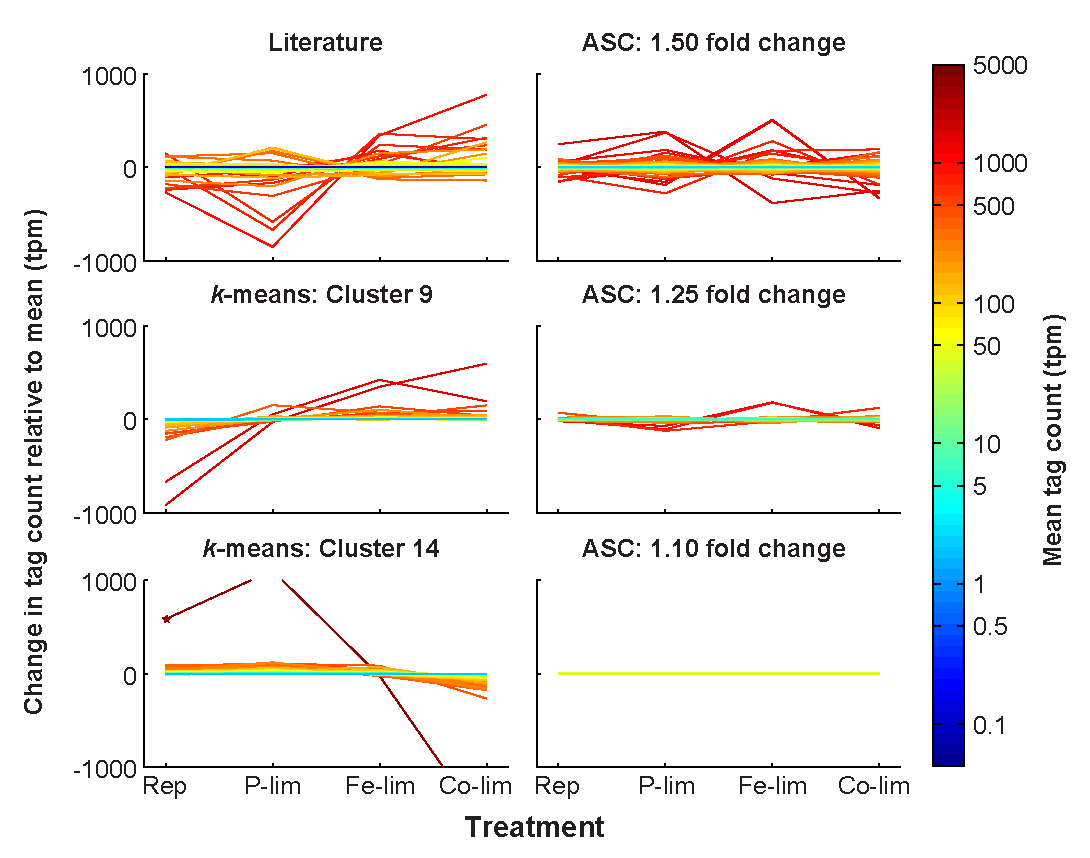
\includegraphics[width=1\textwidth]{Images/C2_Figure1_v6.pdf}
    \caption[Expression patterns of putative reference genes]{Expression patterns of putative reference genes identified through literature-based searches, $k$-means clustering, and ASC analysis. Through literature-based searches, a total of 101 genes homologous to reference genes from previous studies on plants and algae were identified in \textit{T. pseudonana} and plotted to indicate deviation and mean TPM (Literature). $K$-means clustering was applied to the 7380 genes and Cluster 9 (243 genes) and Cluster 14 (466 genes) possessed the genes with the most stable expression pattern across the four treatments. Genes from these clusters are plotted to indicate deviation and mean TPM ($k$-means: Cluster 9; $k-$means: Cluster 14). ASC was used to assess statistical significance (post-$p < 0.1$) of fold changes of 1.10, 1.25, and 1.50 for each treatment relative to the replete control. Genes from these fold change bins are plotted to indicate deviation and mean TPM (ASC: 1.50 fold change; ASC: 1.25 fold change; ASC 1.10 fold change). For a fold change of 1.10, two genes, both hypothetical proteins, (NCBI: 7446346 and 7452192) passed the post-$p < 0.1$ cutoff, and represent the most stable genes based on the ASC analysis (\ref{DS23}). For each of the six classes of putative reference genes, tag counts were normalized to total library size (in TPM) and are plotted relative to the mean for each of the four treatments: Replete (Rep), P-limited (P-lim), Fe-limited (Fe-lim), and co-limited (Co-lim). The color of the line correlates to the mean normalized tag count. A star marks a gene (NCBI: 7451632) in Cluster 14 that is not on the scale of expression for P-limited (1104.7 TPM) and co-limited (-1664.9 TPM) treatments. }
  \label{fig:c2f1}
\end{figure}

The high-throughput transcript dataset was analyzed with $k$-means clustering. Prior to performing $k$-means cluster analysis, FOM optimization was run and found to be minimized at $k=1$5. Thus, $k$-means analysis was run under the Pearson correlation coefficient for $k=15$, yielding 15 clusters, for which the intra-cluster variation was minimized (Figure \ref{fig:a1f2}). Of the 15 clusters produced (ranging in size from 162 to 954 genes), Cluster 4 (433 genes), Cluster 9 (243 genes), and Cluster 14 (466 genes) had candidate reference genes based on a low magnitude of change associated with the expression patterns in those clusters (Figure \ref{fig:a1f2}). However, Cluster 4 showed a clear pattern of differential regulation (downregulated in the replete and upregulated in the co-limited), and as such it was not considered to be an optimal candidate cluster and was excluded from additional analyses. Both Cluster 9 and Cluster 14 consisted of genes with a wide range in mean TPM values (1.74 to 4191.91 TPM), with relatively small deviations from the mean value (Figure \ref{fig:c2f1}; \ref{DS22}), which stands in contrast to other clusters that had definite treatment driven expression patterns (Figure  \ref{fig:a1f2}). Despite the relatively small deviations from the mean value, genes in Clusters 9 and 14 displayed both clear patterns of regulation, as demonstrated by the average change in tag count relative to the mean (Figure \ref{fig:c2f2}) and the presence of ``outlier'' genes with differential expression such as NCBI: 7451632, which was downregulated in the co-limited treatment for Cluster 14 (Figure \ref{fig:c2f1}; \ref{DS22}). \par

%Figure 2: Deviation from the mean
\begin{figure}[h!]
  \centering
    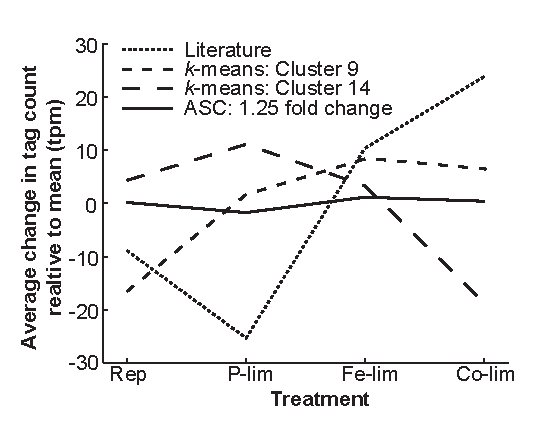
\includegraphics[width=0.65\textwidth]{Images/C2_Figure2_v6.pdf}
    \caption[Average deviation from the mean level of expression for putative reference genes]{Average deviation from the mean level of expression for all genes found with literature-based searches, $k$-means clustering, and ASC analysis of 1.25 fold change. The average change in tag count from the mean expression (TPM) for all the genes identified through literature-based searches for genes homologous to known reference genes from the literature $(n = 101)$, $k$-means clustering from Cluster 9 $(n = 243)$ and Cluster 14 (n = 466), and ASC analysis identifying genes demonstrating a 1.25 fold change with a post-$p < 0.1$ $(n = 179)$. The mean standard deviations for the four cases are as follows: Literature (92.62 TPM), Cluster 9 (41.66 TPM), Cluster 14 (43.12 TPM), and ASC (14.24 TPM). The mean TPM is plotted for the four treatments: Replete (Rep), P-limited (P-lim), Fe-limited (Fe-lim), and co-limited (Co-lim).}
  \label{fig:c2f2}
\end{figure}

Adapting ASC to examine stable expression patterns, genes for which the post-$p$ was less than 0.1 (e.g. had less than a 10\% chance of equaling or exceeding the fold change cutoff) were plotted in three low fold change bins: 1.10, 1.25, and 1.50. A post-$p$ of 0.1 was selected as it optimized the dataset for a wide range of mean gene expression values and provided coverage for each of the fold change bins examined (Table \ref{tab:c2t1}). The number of genes in each of the fold change bins increased with increasing value of fold change. For example, two genes passed the 1.10 cutoff, 179 genes passed the 1.25 cutoff, and 1375 genes passed the 1.50 cutoff. With the increase in the number of genes came an increase in the variation from the mean of the normalized tag counts (Figure \ref{fig:c2f1}; \ref{DS23}). \par
The bin with the 1.10 cutoff had two genes (NCBI: 7446346 and 7452192), which are both hypothetical proteins (Figure \ref{fig:c2f1}). A BLASTn search of 7446346 against the nr NCBI database yielded 69\% identity over 251 base pairs (e-value, 1e-13) to a hypothetical protein (NCBI: CP000544.1) from \textit{Halorhodospira halophila}, a salt-tolerant purple bacterium, and 69\% identity over 232 base pairs (e-value, 1e-12) to a hypothetical protein (NCBI: CP001905.1) from \textit{Thioalkalivibrio} sp. K90mix, also a salt-tolerant chemolithoautotrophic bacteria. BLASTp searches of 7452192 showed the highest identity hits to hypothetical proteins from \textit{Aureococcus anophagefferens} (NCBI: EGB11506.1; 31\% identity; e-value, 2e-21) and from \textit{Chlorella variablis} (NCBI: EFN56803.1; 24\% identity; e-value, 7e-11).\par




The 1.25 fold change bin was used for the identification of candidate reference genes as it offered a larger selection than the 1.10 fold change bin without including genes with increased deviations from the mean, as was the case with the 1.50 fold change bin. Thus, the 1.25 fold change category was the focus of the rest of the analyses (\ref{DS23}). Genes in the 1.25 fold change bin showed a broad range of mean normalized tag counts ranging from 7 to over 1200 TPM with a median of 41.94 TPM, providing for the selection of genes with different levels of constitutive expression in the cell (Figure \ref{fig:c2f1}). Notably, the median of the average tag counts of the genes in the ASC 1.25 fold change bin was 41.94 TPM, which is much higher than that of both Cluster 9 and Cluster 14 with median values of 14.18 TPM and 21.93 TPM, respectively. \par

\begin{landscape}
\begin{table}[h!]
\centering
\caption{Gene counts for the fold change bins of 1.50, 1.25, and 1.10 across posterior probability cutoffs ranging from 0.01 to 0.20.}
\label{tab:c2t1}
\small
\begin{tabular}{|p{2.2cm}|p{1.25cm}|p{1.25cm}|p{1.25cm}|p{1.25cm}|p{1.25cm}|p{1.25cm}|p{1.25cm}|p{1.25cm}|p{1.25cm}|}
\hline
Fold change & \multicolumn{3}{c|}{1.50}                   & \multicolumn{3}{c|}{1.25}                   & \multicolumn{3}{c|}{1.10}                   \\ \cline{1-10} 
Posterior probability                             & Number of genes & Min. TPM & Max. TPM & Number of genes & Min. TPM & Max. TPM & Number of genes & Min. TPM & Max. TPM \\ \hline
post-$p < 0.2$        & 1649            & 2.11        & 1802.38     & 312             & 2.83        & 1281.15     & 8               & 20          & 176.63      \\ \hline
post-$p < 0.1$         & 1375            & 2.22        & 1802.38     & 179             & 7.06        & 1281.15     & 2               & 51.81       & 105.73      \\ \hline
post-$p < 0.05$       & 1127            & 2.83        & 1802.38     & 122             & 20          & 1281.15     & 1               & 105.73      & 105.73      \\ \hline
post-$p < 0.01$        & 801             & 5.69        & 1802.38     & 62              & 20          & 1281.15     & 0               & NA          & NA          \\ \hline
\end{tabular}
\end{table}
\end{landscape}



	Underlying differences in the magnitude and pattern of expression variation across treatments were identified by examining the average tag count change for each reference gene detection method (Figure \ref{fig:c2f2}). If all genes in a group were perfectly constitutively expressed, the average change in tag count relative to the mean observed would be 0 TPM (e.g. the TPM values across all treatments for each of the genes within a group were the same). The average variation from the mean observed in the literature (ranging from -25.34 to 23.84 TPM) highlighted the differential expression across treatments. The average change in tag count relative to the mean in both Cluster 9 (ranging from -16.56 to 8.47) and Cluster 14 (ranging from -18.72 to 11.11 TPM) clearly demonstrated patterns of regulation across treatments (e.g. the upregulation under P-limitation and downregulation under co-limited observed in Cluster 14). In contrast, the average change in tag count relative to the mean observed in the genes identified through ASC (1.25 fold change with post-$p$ < 0.1), which showed a low magnitude of variation (ranging from -1.732 to 1.613 TPM) and a small mean standard deviation across the four treatments (14.24 TPM). Ultimately, the expression patterns of the majority of the genes identified through literature-based searches and $k$-means clustering were more variable across the \textit{T. pseudonana} test treatments, than those genes identified with ASC.\par	
\begin{figure}[h!]
  \centering
    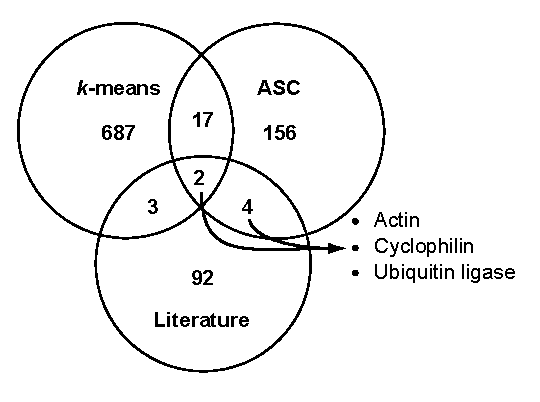
\includegraphics[width=0.75\textwidth]{Images/C2_Figure3_v6_bw.pdf}
    \caption[Comparison of putative reference genes identified through literature, $k$-means clustering, and ASC analysis]{Comparison of possible reference genes found with literature-based searches, $k$-means clustering, and ASC analysis of 1.25 fold change. Venn diagram analysis was used to compare genes identified as candidate reference genes through literature-based homolog searches (totaling 101 genes), with the $k$-means clustering method (genes in Cluster 9 and 14, totaling 709 genes), and with quantitative exclusion by ASC (based on genes demonstrating a 1.25 fold change with a post-$p < 0.1$, totaling 179 genes). The number of genes in each region is reported. The intersection of all ASC and literature-based searches yielded six total genes representing three different gene families: actin (NCBI: 7449411), cyclophilin (NCBI: 7445376), and ubiquitin ligase (NCBI: 7448637, 7450639, 7446724, and 7451971). }
  \label{fig:c2f3}
\end{figure} 
A comparison of the three techniques: literature-based searches, $k$-means cluster selection, and ASC cutoff at 1.25 fold change revealed comparatively few genes in common between the techniques (Figure \ref{fig:c2f3}). Of the 709 genes identified through $k$-means clustering and the 179 genes found through ASC analysis (genes which pass the 1.25 fold change cutoff for post-$p$ < 0.1), 21 genes are shared (Figure \ref{fig:c2f3}), of which six lacked GO annotations or KOG definitions (\ref{DS22}). Between the genes identified through literature and ASC analysis, six genes were held in common; these genes were representative of the general gene classifications: actin (NCBI: 7449411), cyclophilin (NCBI: 7445376), and ubiquitin ligases (NCBI: 7448637, 7450639, 7446724, and 7451971). Only two genes (NCBI: 7448637 and 7446724) were found in common amongst all three methods of reference gene selection, both of which were annotated as putative ubiquitin ligases (\ref{DS21}). \par



\section{Discussion}
	Prior to the availability of high-throughput molecular datasets, reference genes for non-model organisms were selected based on literature reports of stably expressed genes in model organisms. With non-model organisms such as eukaryotic phytoplankton this task is particularly difficult, as stably expressed genes are not readily apparent in the relatively limited molecular literature specific to these organisms. Often the selection of a reference gene relies on information from distantly related organisms under dissimilar conditions, leading to extensive validation work \citep{McDonald2010, Whitney2011a}. Herein, we compared the efficacy of reference gene selection based on the literature as compared to verifiable selection through $k$-means clustering and ASC analysis of high-throughput transcriptome data in \textit{T. pseudonana} across four nutrient treatments (replete, P-limited, Fe-limited, and co-limited). These treatments are of environmental relevance as both P and Fe are major drivers of diatom physiological ecology and consequently carbon fixation \citep{Moore2004}. Additionally, P and Fe often occur concurrently at very low concentrations in marine systems and have been found to be independently co-limited, or mutually exclusive biochemically \citep{Saito2008}.\par
    Our literature-based search of relative gene expression studies from 12 algae and plants yielded 18 general reference gene categories, for which 101 homologs in the \textit{T. pseudonana} genome were identified (\ref{DS21}). While some of these genes demonstrated stable expression (e.g. actin, cyclophilin, and ubiquitin conjugating enzymes), the vast majority displayed some form of differential expression in the treatments examined herein. Furthermore, there was considerable heterogeneity of expression among the different gene copies of actin, cyclophilin, and ubiquitin conjugating enzymes, demonstrating that not all genes within a gene family are stably expressed. These data underscore that a literature-based selection of reference genes necessitates validation across all treatments of interest \citep{Vandesompele2002, Pfaffl2004}. \par
	Differential expression patterns in high-throughput datasets are often analyzed with clustering methods, such as hierarchical or $k$-means clustering \citep{Dhaeseleer2005}. Rather than using a clustering method for the identification of differential expression patterns, here it is applied to identify constitutively expressed genes. The $k$-means clustering algorithm was chosen as it is a top-down or partition-based approach to gene clustering that is not hierarchical and requires few assumptions about the data \citep{Hartigan1979}. Several of the 709 putative reference genes identified by $k$-means analysis (from Clusters 9 and 14) were clearly differentially regulated, with large deviations from the mean expression level. The presence of outliers is to be expected using the $k$-means method, for it is a pattern-based method and all genes must be placed into one of the partitioned $k = 15$ clusters. Thus, optimal placement of a gene is not always guaranteed. As with a finite number of clusters, the assignment of a gene is often forced. For example, even genes in Cluster 9 and 14 were subject to strong patterns of regulation, with both clusters demonstrating large average changes in tag count relative to the mean tag count. Arguably, it is better to select a reference gene from a pool of genes that do not share the same pattern of regulation. Therefore, genes uncovered via $k$-means clustering must be manually surveyed to exclude genes with large deviation prior to the selection of a candidate reference gene.\par
	In lieu of clustering approaches, other studies have used statistical parsing of ESTs in tomato plants \citep{Coker2003} and Affymetrix whole-genome GeneChip data from \textit{A. thaliana} \citep{Czechowski2005} and humans \citep{DeJonge2007a} to identify reference genes that have small deviations from the mean of replicated treatments. In contrast to these and other statistical methodologies typically applied to high-throughput sequence data with replication, the Bayesian approach to gene expression analysis, ASC, allowed for selection of candidate genes based on a statistical cutoff rather than cardinality. Though typically used for the identification of differentially expressed genes, the function of ASC was reversed in this study by lowering the post-$p$ cutoff. Genes for which post-$p < 0.1$ for a specified fold change were targeted, meaning that genes that were unlikely to have made that fold change were selected. The 1.25 fold change bin yielded the most options for candidate reference genes without sacrificing stability of expression (as was seen in the 1.50 fold change bin). \par
	ASC provides a method of identifying reference genes with expression levels similar to those of target genes. For example, the mean normalized tag counts of genes identified using ASC were broad (from 7 to over 1200 TPM), providing the opportunity for reference gene expression to be generally matched with target gene expression. Current studies frequently employ reference genes for endogenous control that have very high levels of expression across all treatments, such as ACT1 (NCBI: 7449411) in \textit{T. pseudonana} (which has a mean expression value of 1024.1 TPM in this data set), yet these highly expressed genes might not be optimal for studies of genes with low levels of expression or when multiplexing targets in probe-based RT-qPCR analysis. \par
	High-throughput transcript datasets also allow the selection of reference genes to move beyond the confines of gene annotation and previously identified reference genes. In fact, the two genes with the most stable expression in the 1.10 fold change bin are hypothetical, with no clear annotation. Of the 179 genes that passed the 1.25 fold change cutoff with ASC, 44 lacked both GO and KOG annotations. A large percentage of the 11,390 genes in the \textit{T. pseudonana} genome are annotated as hypothetical proteins \citep{Armbrust2004, Mock2008}, and here we show a number of them are stably expressed across the target conditions. This has been seen with model organisms, where a good majority of constitutively expressed genes fall outside the bounds of preconceived ``housekeeping'' genes \citep{Czechowski2005, DeJonge2007a}. By using a Bayesian approach such as ASC, hypothetical proteins can be chosen as reference genes. \par
    Comparison of the putative reference genes recovered using ASC to previous studies served to cross-validate the ASC approach. Actin (ACT1, NCBI: 7449411) has been validated in the literature as a suitable reference gene for relative expression studies of \textit{T. pseudonana} under Fe-limitation \citep{Whitney2011a}, a treatment considered in this study, and was one of the 179 genes passing the ASC 1.25 fold change cutoff. Additionally, only five of the 179 genes with stable expression found with ASC were identified as differentially expressed in a study of \textit{T. pseudonana} under additional treatments to those described here (e.g. nitrogen limitation, silica limitation, etc.) \citep{Mock2008} (\ref{DS24}). Of the five, only one gene (NCBI: 7451974) was identified as differentially expressed under Fe-limitation, a condition examined in this study. Taken together, this validates the genes identified with ASC using alternative data and methods, and suggests that the ASC-detected genes are globally stable across many different conditions for \textit{T. pseudonana}. However, one of the two genes identified in the 1.10 fold change bin (NCBI: 7446346) was identified as significantly down-regulated under nitrogen limitation by \citet{Mock2008}. This highlights the importance of validating genes across all treatments of interest prior to their use as reference genes. \par
	Notably, the $k$-means and ASC dataset revealed only 21 genes in common. The 179 genes found through ASC were, in fact, distributed fairly evenly across all of the 15 clusters. The lack of intersection observed between the two datasets is likely related to the parsing ability inherent in $k$-means clustering. The $k$-means approach is highly driven by patterns of differential regulation, but does not consider the significance of that regulation (e.g. genes that are not significantly upregulated are placed in a cluster with genes that are significantly upregulated). Thus, the stably expressed genes that were identified by ASC, though not displaying major patterns of regulation, were clustered based on minor patterns in variation of gene expression. Therefore, while $k$-means clustering provides a global view of commonalities in gene expression patterns, ASC is more robust at identifying reference genes.\par
	Eight genes were common between the ASC and literature-based searches, which were distributed across three general gene classes: actin (NCBI: 7449411), cyclophilin (NCBI: 7445376), and ubiquitin ligases (NCBI: 7448637, 7450639, 7446724, and 7451971). For those interested in identifying suitable reference genes for studies in \textit{T. pseudonana} but lack transcriptome datasets across the treatments of interest, these eight genes may serve as good tentative reference genes as they are verified in this study and have been identified as stable in many other organisms under many conditions. In particular, ubiquitin ligases/conjugating enzymes have been used as reference genes in several studies involving other algae, namely, \textit{Aureococcus anophagefferens}, \textit{Phaeodactylum tricornutum}, and \textit{Prorocentrum minimum} \citep{Siaut2007, McGinn2008, Guo2012, Wurch2011, Berg2008}, and with further analysis may represent particularly good reference genes in the phytoplankton. \par
	Sequence-based transcriptome profiling has become an increasingly useful method for gene discovery and differential expression analysis. Yet, RT-qPCR is still valuable for the examination of detailed trends in expression in both culture and field studies. Here we show that the application of ASC and, to a lesser extent, $k$-means clustering can be used to successfully screen transcriptome data for potential reference genes. The isolation of candidate reference genes using ASC with the 1.25 fold change cutoff for post-$p < 0.1$ was more robust and stringent at excluding differentially expressed genes than both the literature-based searches and $k$-means clustering. Based on these data for \textit{T. pseudonana}, it was shown that ACT 1 and ubiquitin ligase may be useful reference genes. Yet, in addition to these common reference genes, the data demonstrate that there are many more stably expressed genes (both annotated and hypothetical) to choose from for expression studies in this and potentially other diatoms. Notably, this survey focused only on variation in P and Fe supply, so these genes may not transfer to studies of other nutritional drivers or other physical forces, such as light intensity or temperature. As more transcriptome data are generated for phytoplankton, ASC can be employed without sequence replicates, to identify reference genes for other phytoplankton under various conditions. Additionally, the suite of genes identified through these analyses might allow for better multi-gene normalization analysis that would provide for the detection of smaller fold changes with certainty \citep{Vandesompele2002, Czechowski2005}.\par




\appendix
\chapter{Supplemental Information}

\raggedbottom


%%%%%%%%%%%%%%%%%%%%%%%%%%%

%%%%%%%%%%%%%%%%%%%%%%%%%%%_________________CHAPTERTWO_________________%%%%%%%%%%%%%%%%%%%%%%%%%%%

%%%%%%%%%%%%%%%%%%%%%%%%%%%
\clearpage
\section{Appendix for Chapter 2}
\subsection{Supplemental Figures}
%Supplemental Figure 1: Histogram of TPM distribution
\begin{figure}[h!]
  \centering
    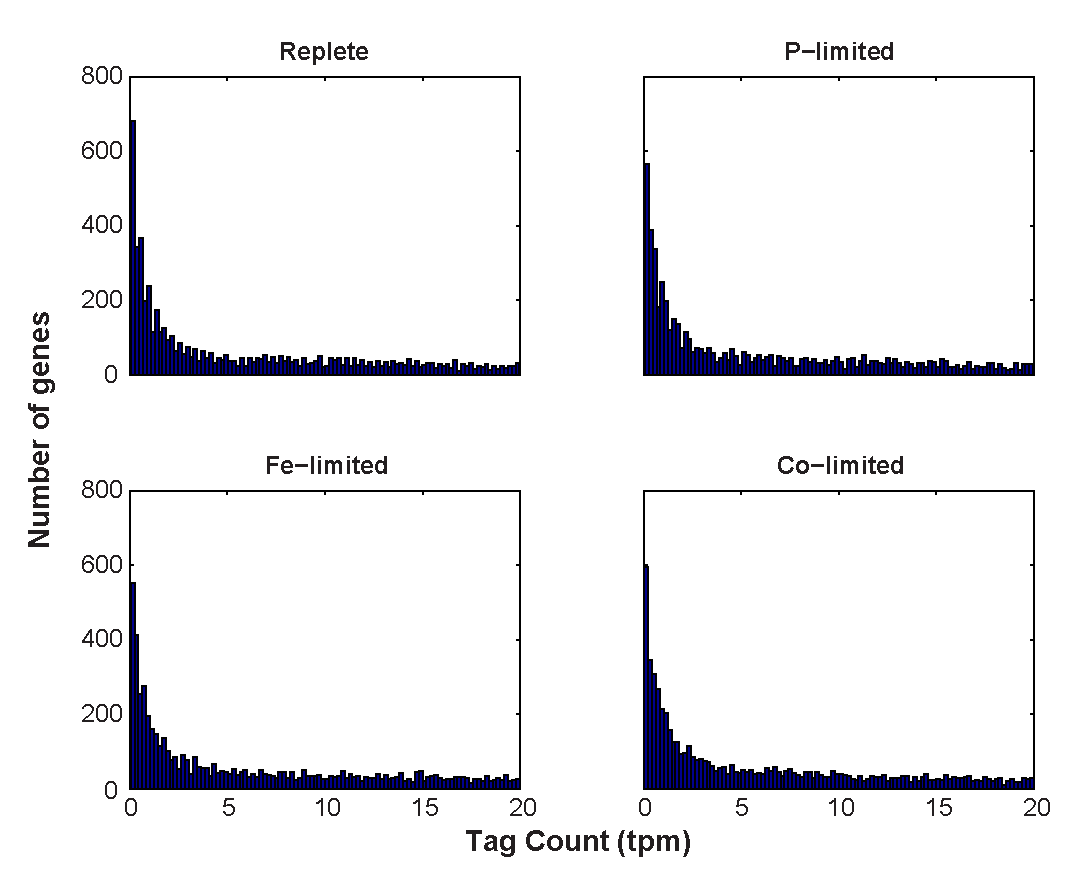
\includegraphics[width=1\textwidth]{Images/C2_FigureS1_v6.pdf}
    \caption[Distribution of normalized tag counts across treatments]{Histogram analysis of the distribution of normalized tag counts (TPM) for each gene across each of the four treatments (Replete, P-limited, Fe-limited, and co-limited). The abundance of normalized tag counts (TPM) was assessed, tallying the total number of genes with a given tag count. Only tag counts less than 20 are depicted to aid the visualization of the inflection in the data at 2.5 TPM.}
  \label{fig:a1f1}
\end{figure}

%Supplemental Figure 2: K-means clusters (all)
\begin{landscape}
   \null         %%<---- this is needed
   \vfill        %%<-----here
   \centering 
    \begin{figure}
    \centering
        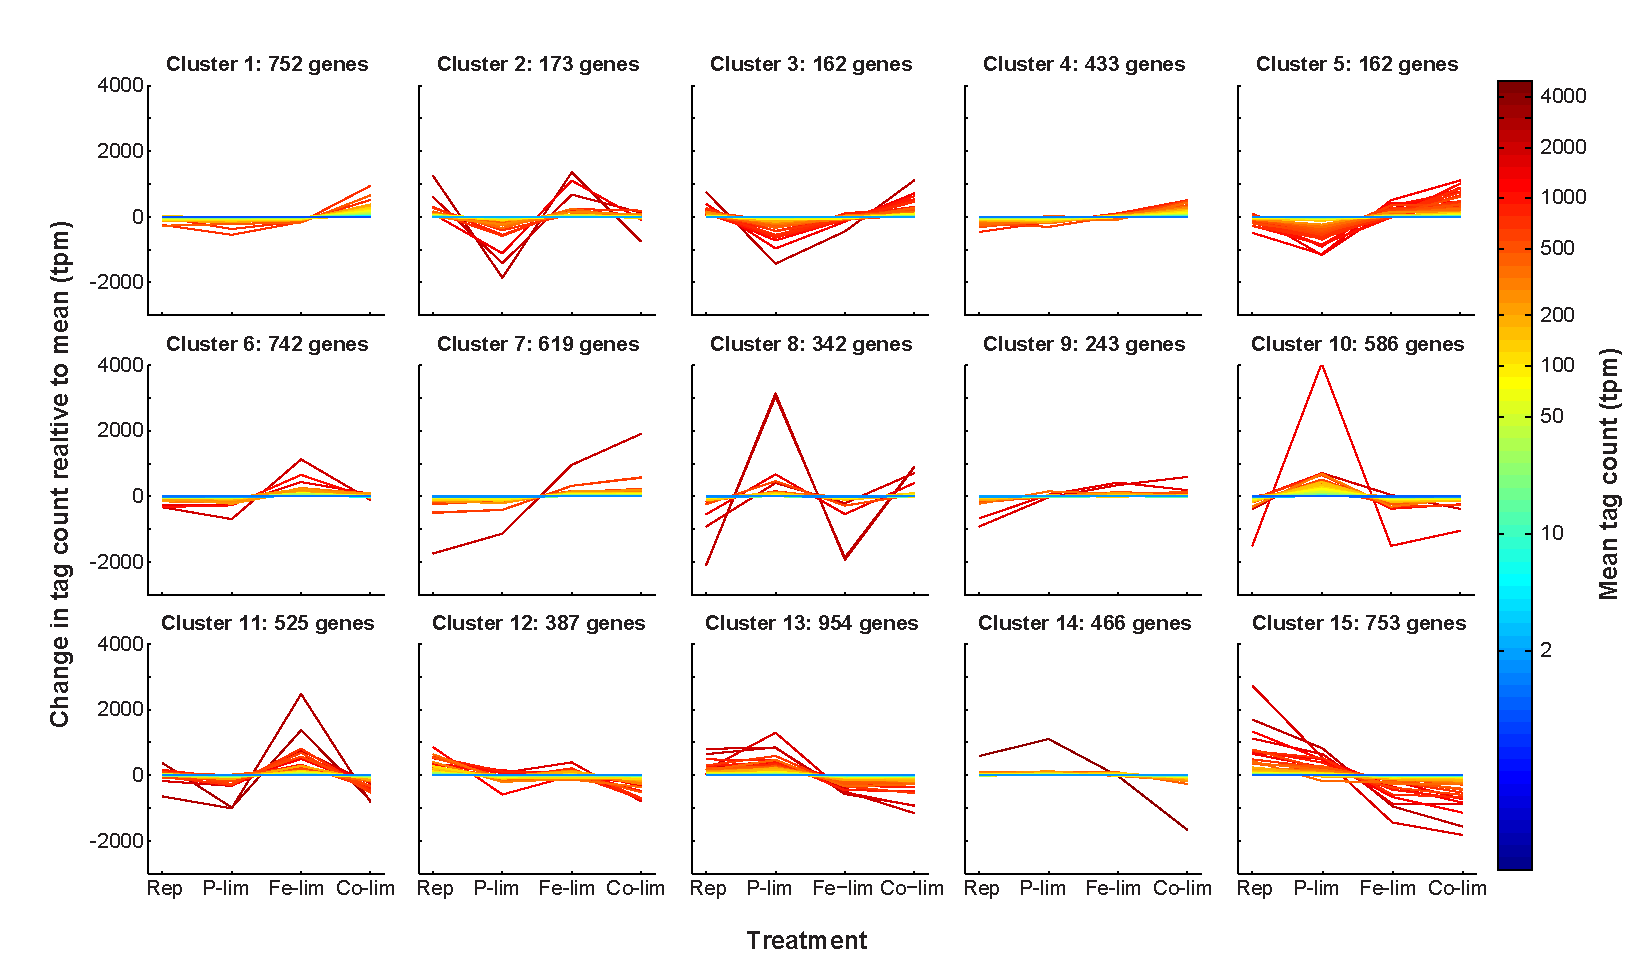
\includegraphics[width=1\textwidth]{Images/C2_FigureS2_v6.pdf}
        \caption[$K$-means clustering of normalized genes]{$K$-means clustering of normalized genes. The 7380 genes that passed the 2.5 TPM cutoff were clustered into 15 clusters using the $k$-means algorithm under the Pearson correlation coefficient. Tag counts normalized to total library size (in TPM) for each gene are plotted relative to the mean (indicated by the color of the line) for each of the four treatments: Replete (Rep), P-limited (P-lim), Fe-limited (Fe-lim), and co-limited (Co-lim).}
    \label{fig:a1f2} 
    \end{figure}
    \vfill        %%<----- and here
\end{landscape}

\clearpage
\newpage

%%%%%%%%%%%%%%%%%%%%%%%%%%%

%%%%%%%%%%%%%%%%%%%%%%%%%%%_________________CHAPTERTHREE_________________%%%%%%%%%%%%%%%%%%%%%%%%%%%

%%%%%%%%%%%%%%%%%%%%%%%%%%%


\section{Appendix for Chapter 3}
\subsection{Supplemental Figures}

%Supplemental Figure 1: Cell counts in NB 
\begin{figure}[h!]
  \centering
    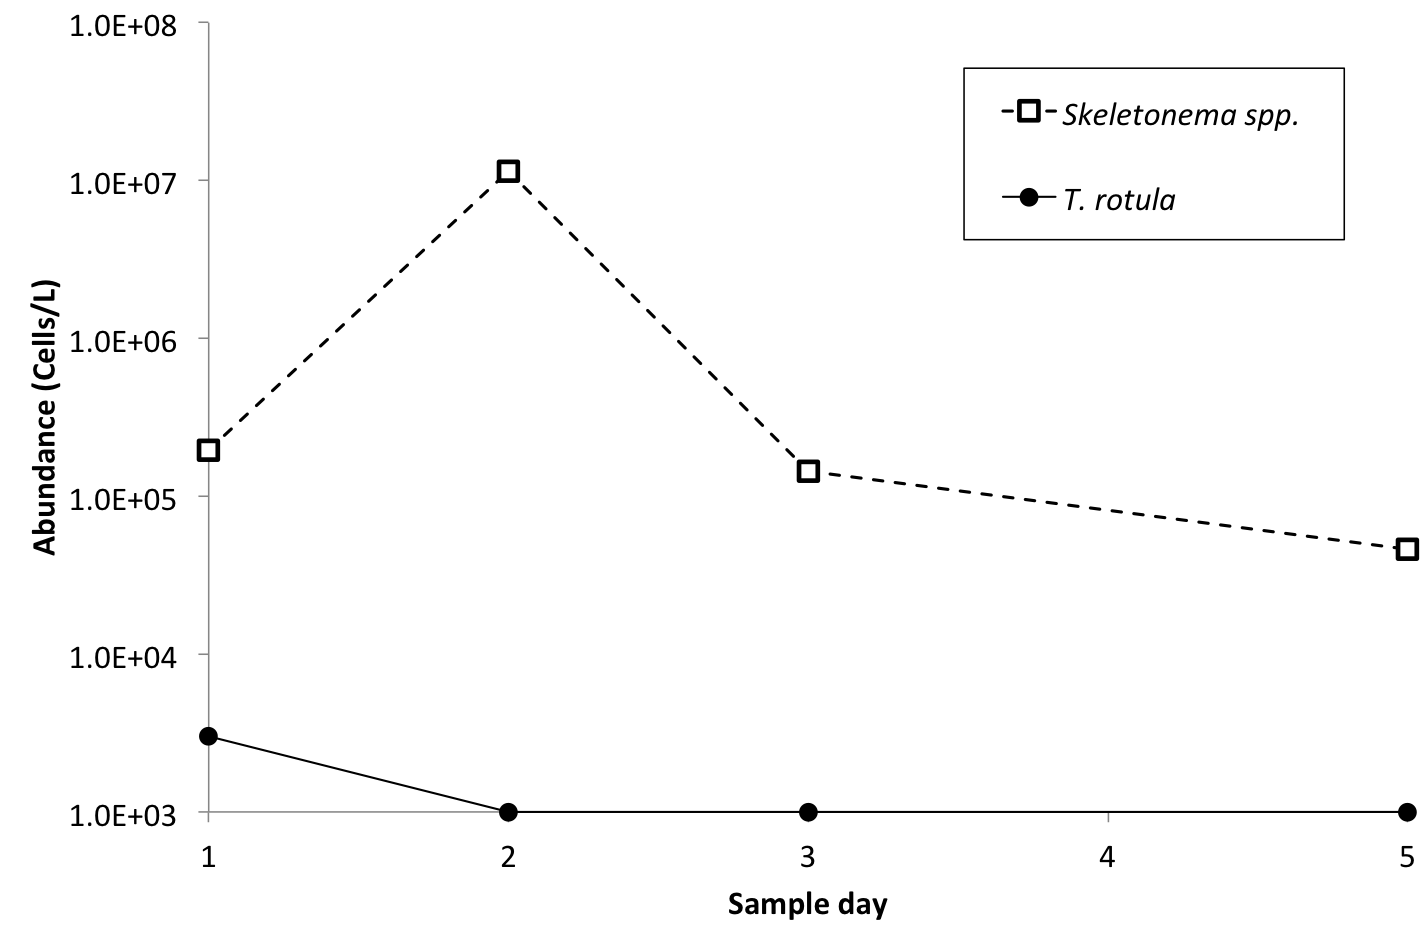
\includegraphics[width=1\textwidth]{Images/C3_SFigure1_CellCounts.png}
    \caption[Cell counts in Narragansett Bay during the spring of 2012]{Abundance estimation from cell counts of \textit{Skeletonema} spp. and \textit{T. rotula} across the five sample points during the spring of 2012. }
  \label{fig:a3f1}
\end{figure}


%Supplemental Figure 2: KEGG linear correlation
\begin{figure}[p!]
  \centering
    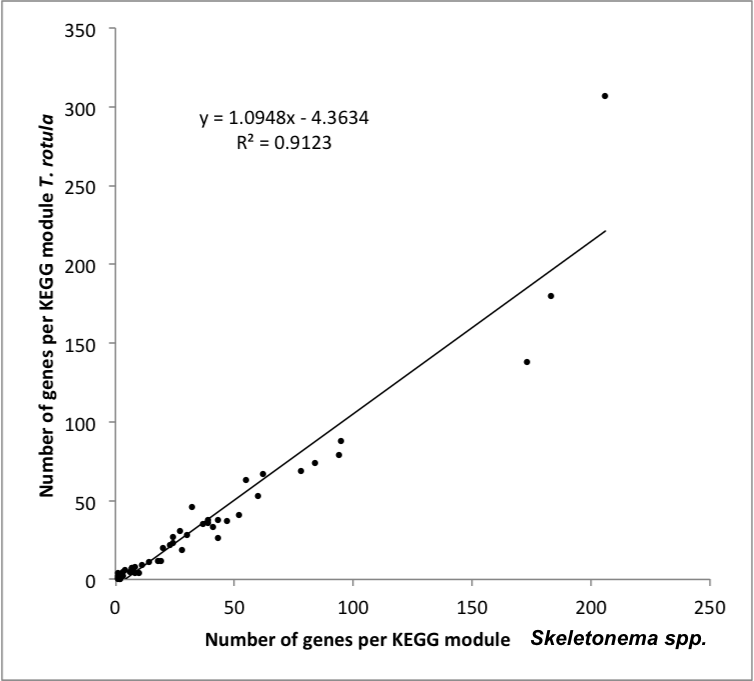
\includegraphics[width=1\textwidth]{Images/C3_SFigure2_KEGGModuleGeneContent2.png}
    \caption[Comparison of KEGG module content between \textit{Skeletonema} spp. and \textit{T. rotula} ]{Total number of genes assigned to each KEGG module for \textit{Skeletonema} spp. and \textit{T. rotula}.}
  \label{fig:a3f2}
\end{figure}


%Supplemental Figure 3: Hierarchical clustering of S and T across time
\begin{figure}[p!]
  \centering
    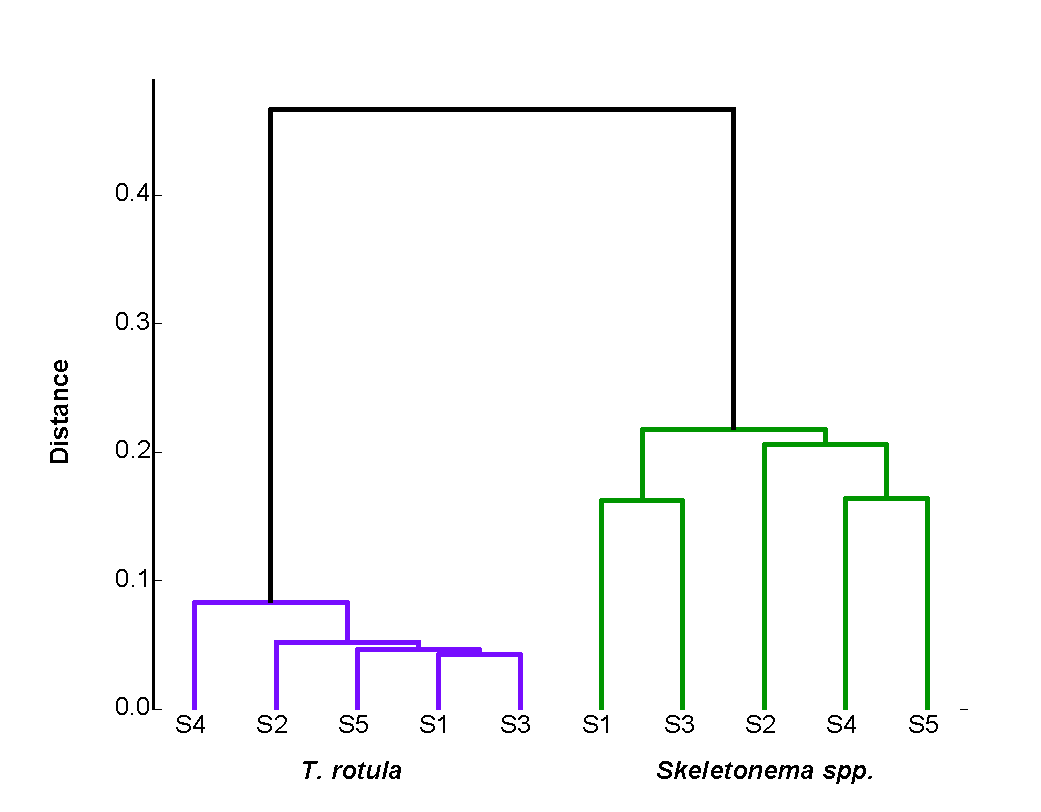
\includegraphics[width=1\textwidth]{Images/C3_SFigure3_Dendrogram.pdf}
    \caption[Hierarchical clustering of QMF signatures across species and samples]{Dendrogram depicting hierarchical clustering of samples based on relative expression of KEGG modules (Figure 2) across the five samples S1-S5 for \textit{Skeletonema} spp. and \textit{T. rotula}.}
  \label{fig:a3f3}
\end{figure}

%Supplemental Figure 4: Stable gene expression across time
\begin{figure}[p!]
  \centering
    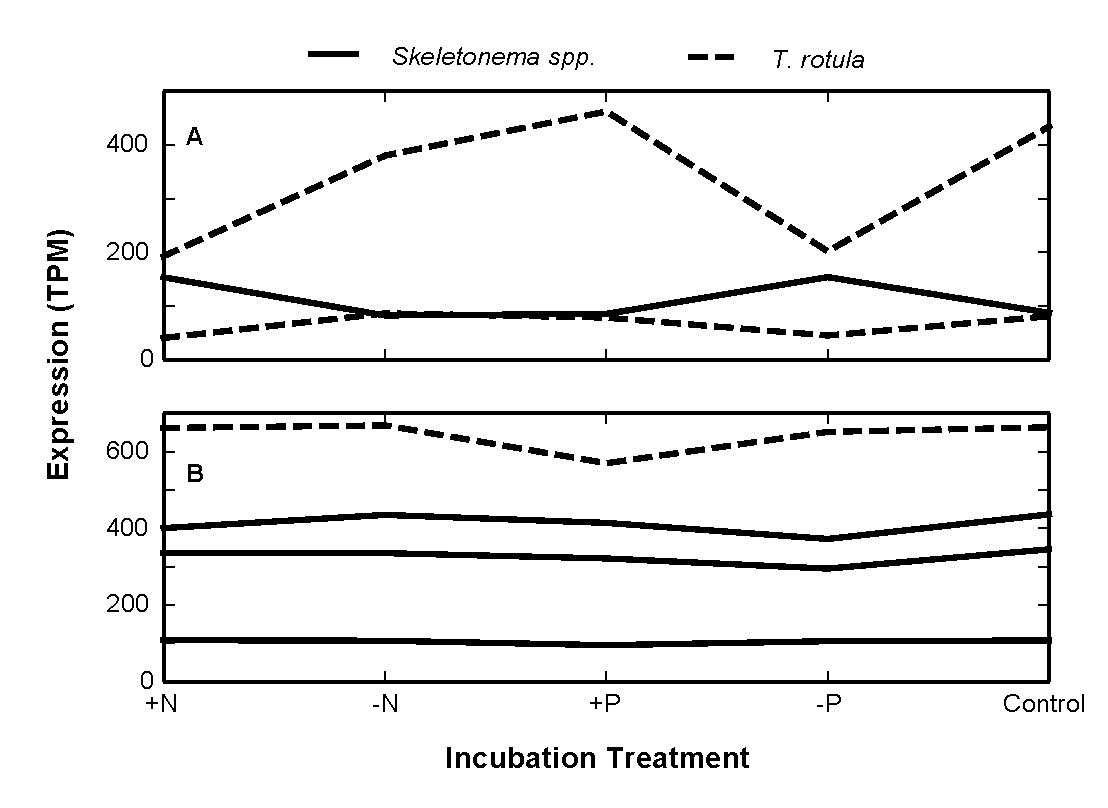
\includegraphics[width=1\textwidth]{Images/C3_SFigure4_StableGenePlot_wActin.pdf}
    \caption[Expression of stable reference genes in the field]{Expression of stable reference genes identified based on literature and statistical parsing in nutrient amendment incubation. (A) The expression in tags per million ($TPM$) of stable reference genes identified in \textit{T. rotula} (dashed line) and \textit{Skeletonema} spp.  (solid lines) based on homology (e-value < 1e-5) to a known reference genes in \textit{T. pseudonana}, ACT1 (Thaps\_25772), in nutrient incubations. (B) Also shown are reference genes identified in the incubation experiments, using statistical analysis of sequence counts \citep{Alexander2012, Wu2010}, and nutrient incubations }
  \label{fig:a3f4}
\end{figure}

%Supplemental Figure 5: RR gene composition
\begin{figure}[p!]
  \centering
    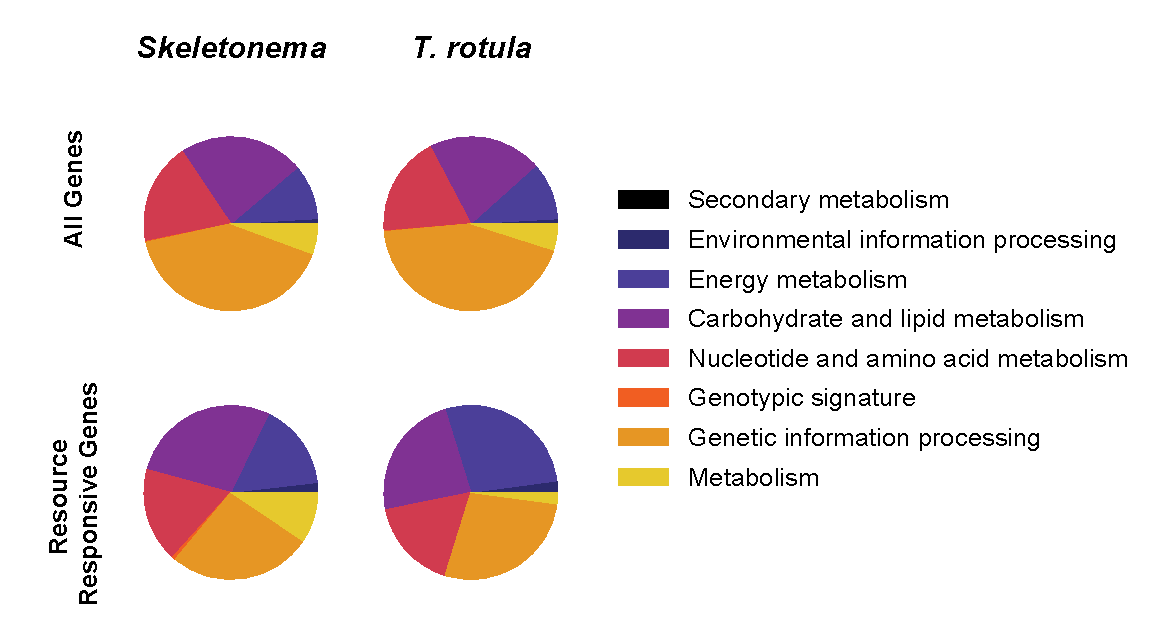
\includegraphics[width=1\textwidth]{Images/C3_SFigure5_RR_All_Genes_Pie.pdf}
    \caption[Functional compoosition of the reference transcriptome and resource-responsive gene sets]{Functional composition of the reference transcriptome and resource-responsive (RR) gene subset for \textit{T. rotula} and \textit{Skeletonema} spp. (A) RR gene sets were identified through cross comparison of like-nutrient incubations (i.e. +N vs. -N and +P vs. -P), using ASC (fold change = 2, post-$p > 0.95$). The relative functional categorization of the reference transcriptomes and RR gene set for \textit{T. rotula} and \textit{Skeletonema} spp. based on KEGG ontology as assigned by KAAS is depicted at the module-level.}
  \label{fig:a3f5}
\end{figure}

%Supplemental Figure 6: Expression of nitrate reductase

\begin{figure}[p!]
  \centering
    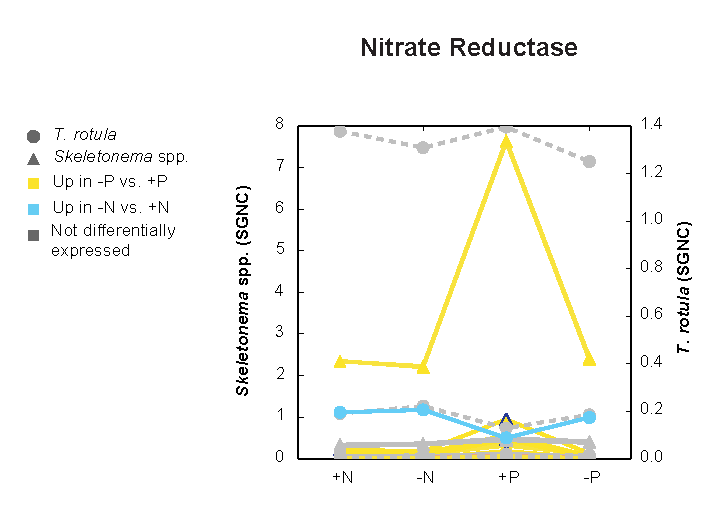
\includegraphics[width=1\textwidth]{Images/C3_SFigure6_SGNC_NitrateReductase.pdf}
    \caption[Relative expression of nitrate reducatses across incubation experiments]{The relative expression in stable gene normalized counts ($SGNC$) of the assimilatory nitrate reductase gene cluster across the incubation experiment treatments. Significance of regulation between the treatments is denoted by the color of the line; organisms are denoted by the shapes of the marker.}
  \label{fig:a3f6}
\end{figure}

%Supplemental Figure 7: Cluster Analysis


\begin{figure}[p!]
  \centering
    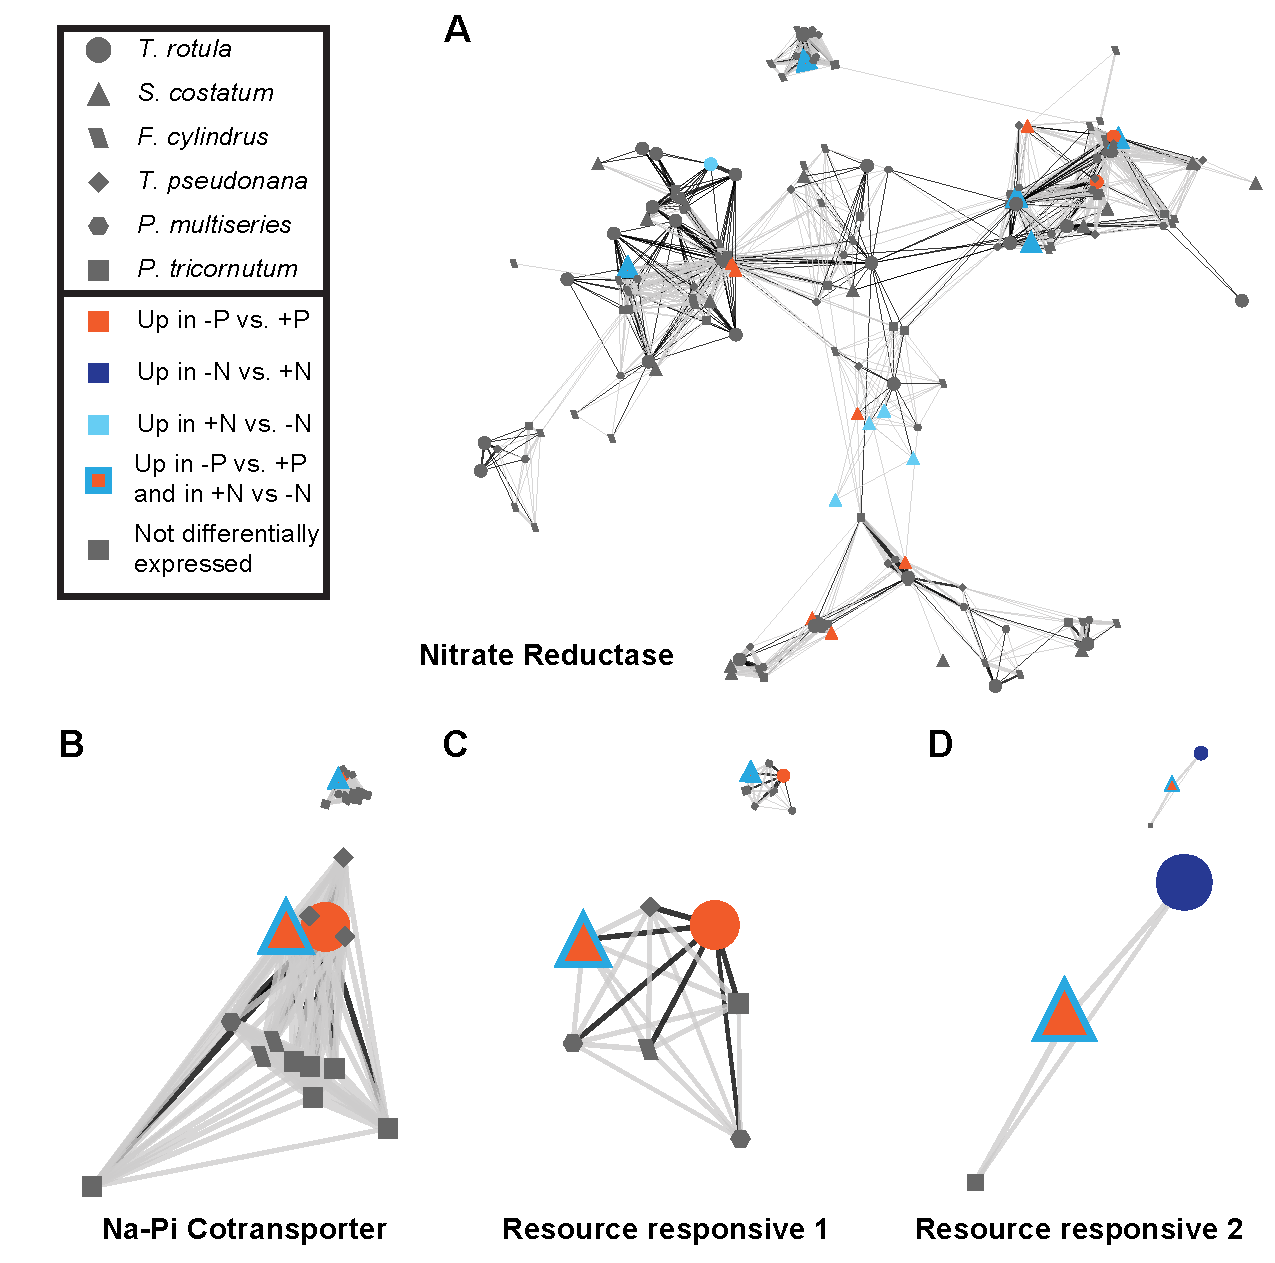
\includegraphics[width=1\textwidth]{Images/C3_SFigure7_ClusterAnalysis_v5.pdf}
    \caption[Gene cluster analysis of nutrient-responsive genes]{Gene cluster known nutrient-responsive genes in \textit{T. pseudonana}: (A) assimilatory nitrate reductase and (B) sodium-phosphate cotransporter and novel resource-responsive (RR) gene families: (C) RR1 and (D) RR2. Transcripts from the transcriptomes of \textit{T. rotula} and \textit{Skeletonema} spp. were clustered based upon relative homology with available diatom genomes: \textit{F. cylindrus}, \textit{P. tricornitum}, \textit{P. multiseries}, and \textit{T. pseudonana}. Symbols indicate different species, while color indicates regulation in the field incubation experiments. Two nodes within a gene cluster are connected by an edge if they share a homologous protein (reciprocal BLAST hit with a minimum of 1e-5 score and minimum 20\% identity). Gene clusters are visualized using an edge-weighted spring-embedded model based on e-value, meaning that genes that are closer together are more similar. The width of the line correlates to the magnitude of the e-value, with lower e-values represented by thicker lines and higher e-values represented by thinner lines.}
  \label{fig:a3f7}
\end{figure}

%Supplemental Figure 8: Conceptual schematic of STD niche space

\begin{figure}[p!]
  \centering
    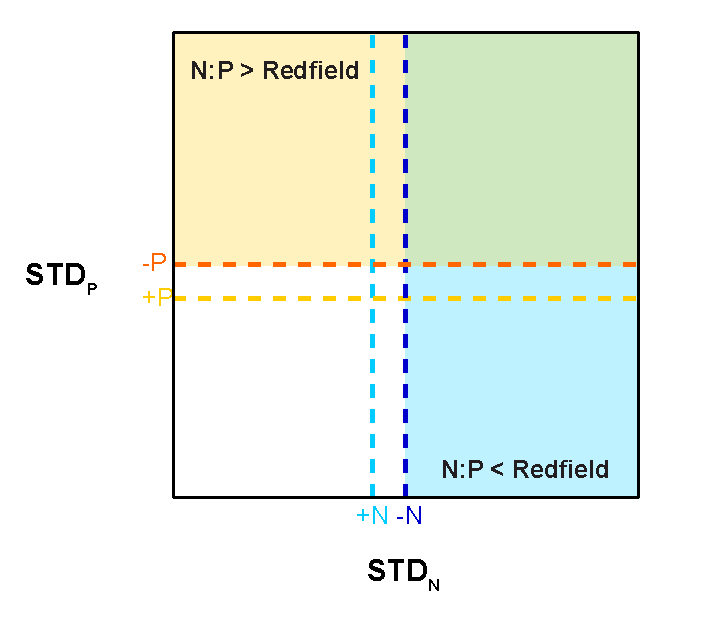
\includegraphics[width=1\textwidth]{Images/C3_SFigure8_Schematic_Quadrants.pdf}
    \caption[Conceptual schemiatic of $STD_N$ plotted against $STD_P$]{A conceptual schematic of $STD_N$ plotted against $STD_P$ hypothesized regions of N:P > Redfield physiology and N:P < Redfield physiology highlighted.}
  \label{fig:a3f8}
\end{figure}


%Supplemental Figure 9: NISP Dn genes
\begin{landscape}
   \centering
   \null         %%<---- this is needed
   \vfill        %%<-----here

	\begin{figure}
  	\centering
    	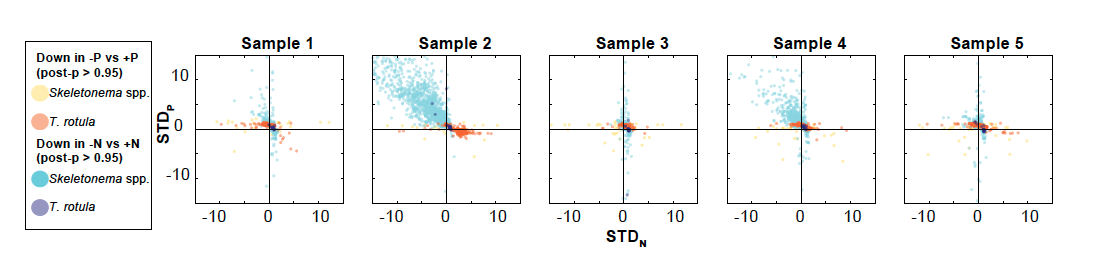
\includegraphics[width=1.3\textwidth]{Images/C3_SFigure9_NISP_DNGenes.png}
    	\caption[Evolution of niche space indexing over for significantly down-regualted genes]{Evolution of niche space indexing over time in Narragansett Bay for \textit{T. rotula} and \textit{Skeletonema} spp.. The stable gene normalized field signal from genes identified as significantly (2-fold change, post$-p > 0.95$) down-regulated in -P vs +P for Skeletonema spp. (yellow) and \textit{T. rotula} (orange) and in -N vs +N for for \textit{Skeletonema} spp. (cyan) and \textit{T. rotula} (dark blue) was proportionalized relative to the expression for those genes in nutrient incubations, yielding the $STD_N$ and $STD_P$. These data are plotted for Sample 1 through Sample 5.}
  	\label{fig:a3f9}
	\end{figure}
    \vfill        %%<----- and here
\end{landscape}

%Supplemental Figure 10: Percentage of RR genes by quadrant

\begin{figure}[h!]
  \centering
    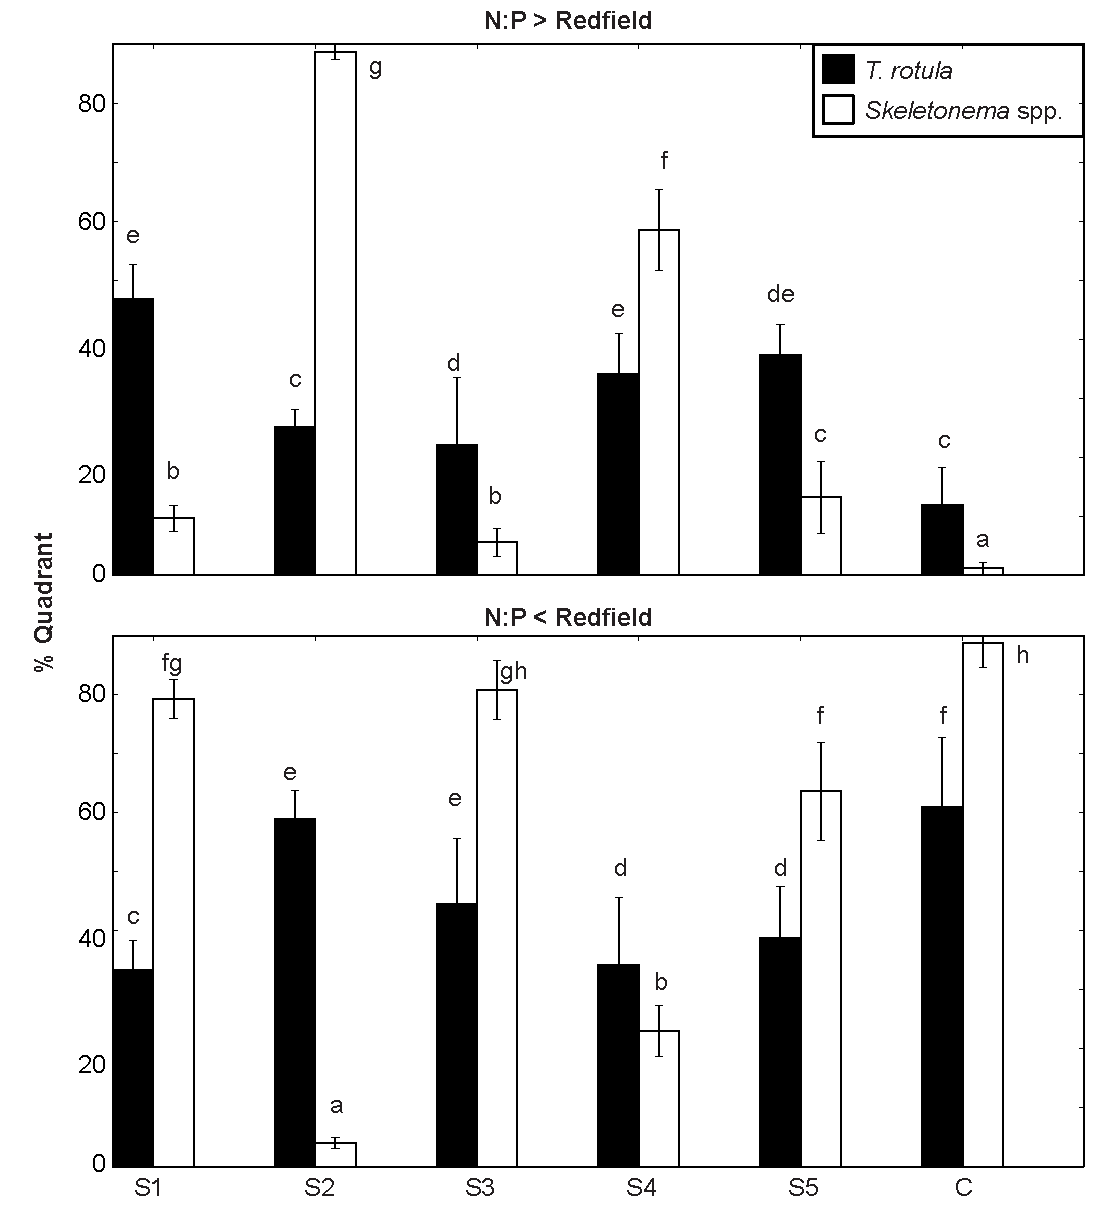
\includegraphics[width=1\textwidth]{Images/C3_SFigure10_BarGraph_Quadrant_2575_stats.pdf}
    \caption[The percentage of identified nutrient responsive genes falling into the N:P > Redfield and N:P < Redfield quadrants with varried cutoffs]{The percentage of identified nutrient responsive genes falling into the N:P > Redfield and N:P < Redfield quadrants for \textit{T. rotula} and \textit{Skeletonema} spp.. The total number of genes falling into the N:P > Redfield quadrant ($STD_P > C$; $STD_N < C$, for $0.25 < C < 0.75$) and the N:P < Redfield quadrant ($STD_P$ < C; $STD_N > C$, for $0.25 < C < 0.75$). The value of C was varied over 10 different values and the average percentages of genes falling into each of the quadrants is depicted above based on the size of the circle at the median $STD_N$ and $STD_P$ for the genes in the quadrant. Similarity of data between species by quadrant was assessed using an analysis of variance (ANOVA) with a generalized linear model. The results from a post hoc Tukey test show the divergence of species across time ($p < 0.05$).}
  \label{fig:a3f10}
\end{figure}

%Supplemental Figure 11: Quadrant localization with varying stable reference genes

\begin{figure}[p!]
  \centering
    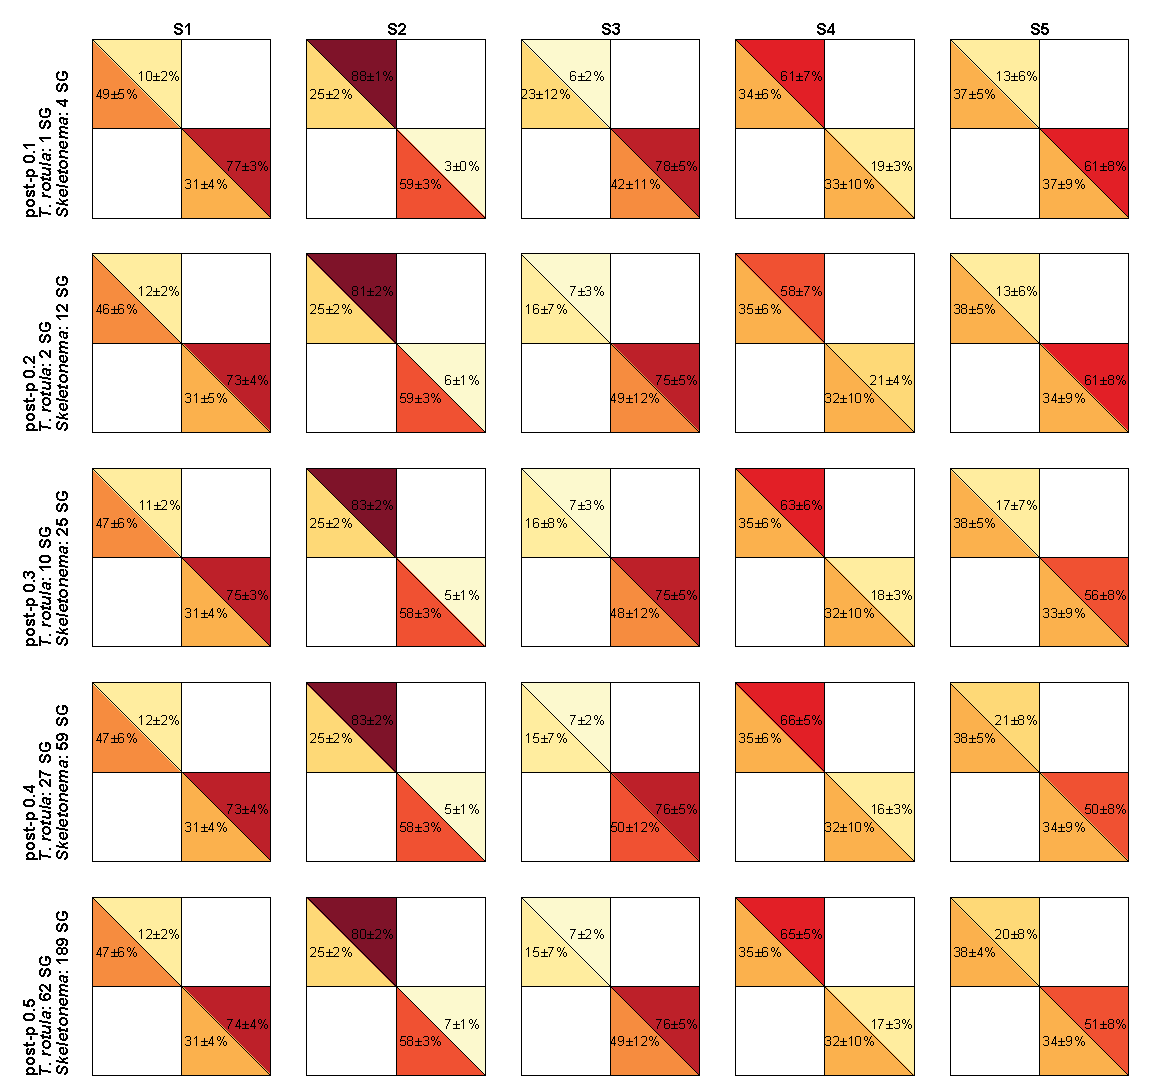
\includegraphics[width=1\textwidth]{Images/C3_SFigure11_Quadrant.pdf}
    \caption[The impact of stable gene selction of quadrant localization]{The impact of stable gene selection on the quadrant localization of the resource responsive gene sets. The posterior probability cutoff used in the selection of stable genes was varied from 0.1 to 0.5 for a fold change of 1.25. The percentage of identified nutrient responsive genes falling into the N:P > Redfield and N:P < Redfield quadrants for \textit{T. rotula} and \textit{Skeletonema} spp. across the five sample points and five posterior probability values is depicted.}
  \label{fig:a3f11}
\end{figure}



\subsection{Supplemental Tables}

%Supplemental Table 1: library stats

\begin{table}[h!]
\centering
\caption[The total number of paired end reads after quality control and trimming and the percentage of reads mapping]{The total number of paired end reads after quality control and trimming and the percentage of reads mapping to the \textit{T. pseudonana} genome, \textit{T. rotula} transcriptome, and \textit{S. costatum} transcriptome.}
\label{tab:a3t1}

\newcolumntype{C}[1]{>{\centering\let\newline\\\arraybackslash\hspace{.5pt}}m{#1}}

\begin{tabular}{|C{2cm}|C{2.5cm}|C{2.5cm}|C{2.5cm}|C{2.5cm}|}
\hline
\multirow{2}{*}{Sample} & \multirow{2}{*}{\parbox{2.5cm}{Total library size (paired end reads)}} & \multicolumn{3}{c|}{Mapped representation in library} \\ \cline{3-5} 
                        &                                                              & \textit{T. pseudonana}      & \textit{T. rotula}      & \textit{S. costatum}     \\ \hline
S1                      & 89455034                                                     & 2.98\%             & 17.50\%        & 33.50\%         \\ \hline
S2                      & 64888267                                                     & 0.41\%             & 11.70\%        & 54.90\%         \\ \hline
S3                      & 103250243                                                    & 0.39\%             & 7.30\%         & 9.00\%          \\ \hline
S4                      & 45370867                                                     & 0.68\%             & 8.80\%         & 8.30\%          \\ \hline
S5                      & 55061692                                                     & 0.88\%             & 10.40\%        & 11.20\%         \\ \hline
Ambient Control         & 51508197                                                     & 0.27\%             & 13.40\%        & 8.00\%          \\ \hline
+N                      & 58626239                                                     & 0.43\%             & 6.10\%         & 5.30\%          \\ \hline
-N                      & 44561851                                                     & 0.41\%             & 8.70\%         & 8.30\%          \\ \hline
+P                      & 51130364                                                     & 0.29\%             & 8.50\%         & 8.00\%          \\ \hline
-P                      & 58834022                                                     & 0.40\%             & 6.60\%         & 6.50\%          \\ \hline
\end{tabular}
\end{table}

%Supplememntal Table 2: nutrient concentrations used in incubations

\begin{table}[h!]
\centering
\caption[Nutrient concentrations used in nutrient amendment incubations. ]{Nutrient concentrations used in nutrient amendment incubations.}
\label{tab:a3t2}
\begin{tabular}{|c|c|c|c|c|c|}
\hline
                                    & \multicolumn{5}{c|}{\textbf{Treatment}}                                                                                              \\ \cline{2-6} 
\multirow{-2}{*}{\textbf{Nutrient}} & Ambient Control          & + P                      & + N                      & - P                      & - N                      \\ \hline
Nitrate                             & \cellcolor[HTML]{C0C0C0} & \cellcolor[HTML]{C0C0C0} & 10 $\mu M$                    & 10 $\mu M$                    & \cellcolor[HTML]{C0C0C0} \\ \hline
Phosphate                           & \cellcolor[HTML]{C0C0C0} & 3 $\mu M$                     & \cellcolor[HTML]{C0C0C0} & \cellcolor[HTML]{C0C0C0} & 3 $\mu M$                     \\ \hline
Silica                             & \cellcolor[HTML]{C0C0C0} & \cellcolor[HTML]{C0C0C0} & \cellcolor[HTML]{C0C0C0} & 68 $\mu M$                    & 68 $\mu M$                    \\ \hline
Iron                                & \cellcolor[HTML]{C0C0C0} & \cellcolor[HTML]{C0C0C0} & \cellcolor[HTML]{C0C0C0} & 4.6 $\mu M$                   & 4.6 $\mu M$                   \\ \hline
Vitamins                            & \cellcolor[HTML]{C0C0C0} & \cellcolor[HTML]{C0C0C0} & \cellcolor[HTML]{C0C0C0} & f/5                      & f/5                      \\ \hline
\end{tabular}
\end{table}


%Supplememntal Table 3: nutrient concentrations used in incubations

\begin{table}[h!]
\centering
\caption[Mapping statistics for \textit{T. rotula} and \textit{S. costatum} transcriptomes]{Total number of contigs in the \textit{T. rotula} and \textit{S. costatum} transcriptomes and the number of genes in each of the differentially regulated and stable groupings.}
\label{tab:a3t3}
\begin{tabular}{|l|l|l|}
\hline
                                                                       & \textit{\textbf{T. rotula}} & \textit{\textbf{S. costatum}} \\ \hline
Number of contigs in transcriptome                                     & 22362                       & 27665                         \\ \hline
Pass 2 TPM cutoff                                                      & 4318                        & 20921                         \\ \hline
Up in -P vs +P                                                         & 249                         & 4754                          \\ \hline
Down in -P vs +P                                                       & 335                         & 52                            \\ \hline
Up in -N vs +N                                                         & 196                         & 9                             \\ \hline
Down in -N vs +N                                                       & 49                          & 1631                          \\ \hline
All differentially regulated (2 fold change, post-$p > 0.95$) & 775                         & 5136                          \\ \hline
Stable genes (1.25 fold change, post-$p < 0.1$)                  & 1                           & 4                             \\ \hline
\end{tabular}
\end{table}




%%%%%%%%%%%%%%%%%%%%%%%%%%%

%%%%%%%%%%%%%%%%%%%%%%%%%%%_________________CHAPTERFOUR_________________%%%%%%%%%%%%%%%%%%%%%%%%%%%

%%%%%%%%%%%%%%%%%%%%%%%%%%%


\clearpage

\section{Appendix for Chapter 4}
\subsection{Supplemental Figures}

%Supplemental Figure 1: Chlorophyll values in experiments and in situ samples 
\begin{figure}[h!]
  \centering
    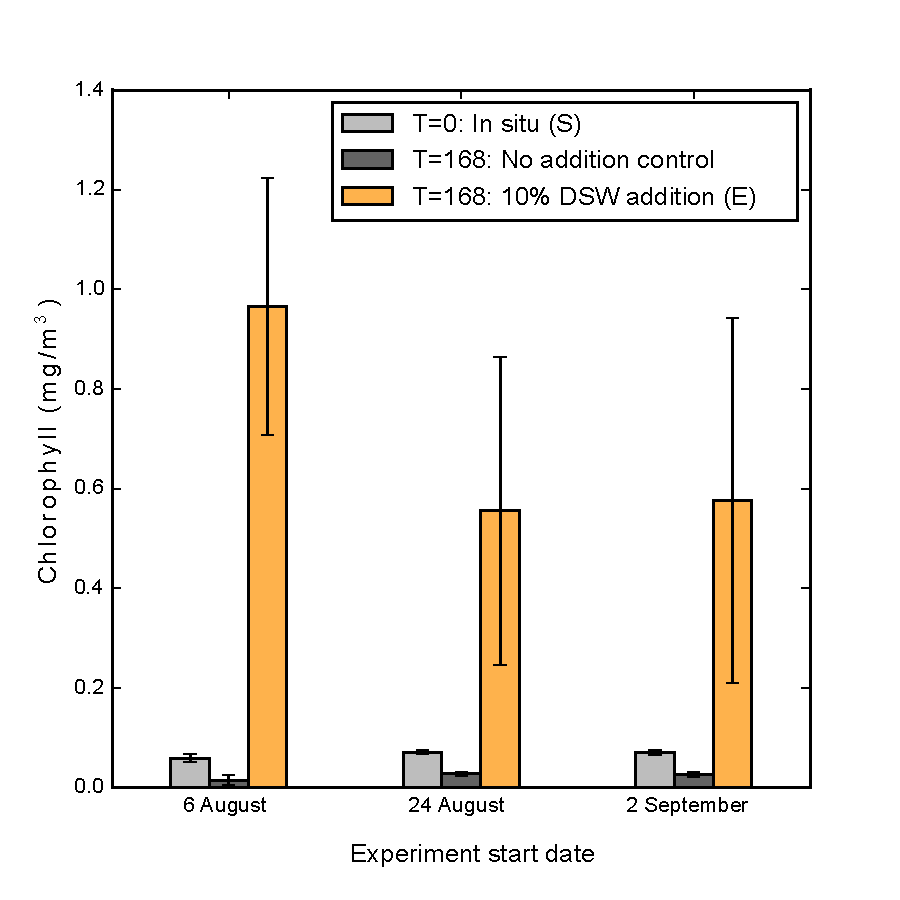
\includegraphics[width=1\textwidth]{Images/C4_FigureS1.pdf}
    \caption[Chlorophyll a of replicated experiments for \emph{in situ} samples, no addition control, and a 10\% deep seawater amendment]{Chlorophyll a of replicated experiments for \emph{in situ} samples (S), a no addition control, and a 10\% deep seawater (DSW) amendment (E). Incubation samples were harvested after 168 hours.}
  \label{fig:a4f1}
\end{figure}


%Supplemental Figure 2: Rank abundance shifts in species composition of diatoms, haptophytes and dinoflagellates

\begin{figure}[p!]
  \centering
    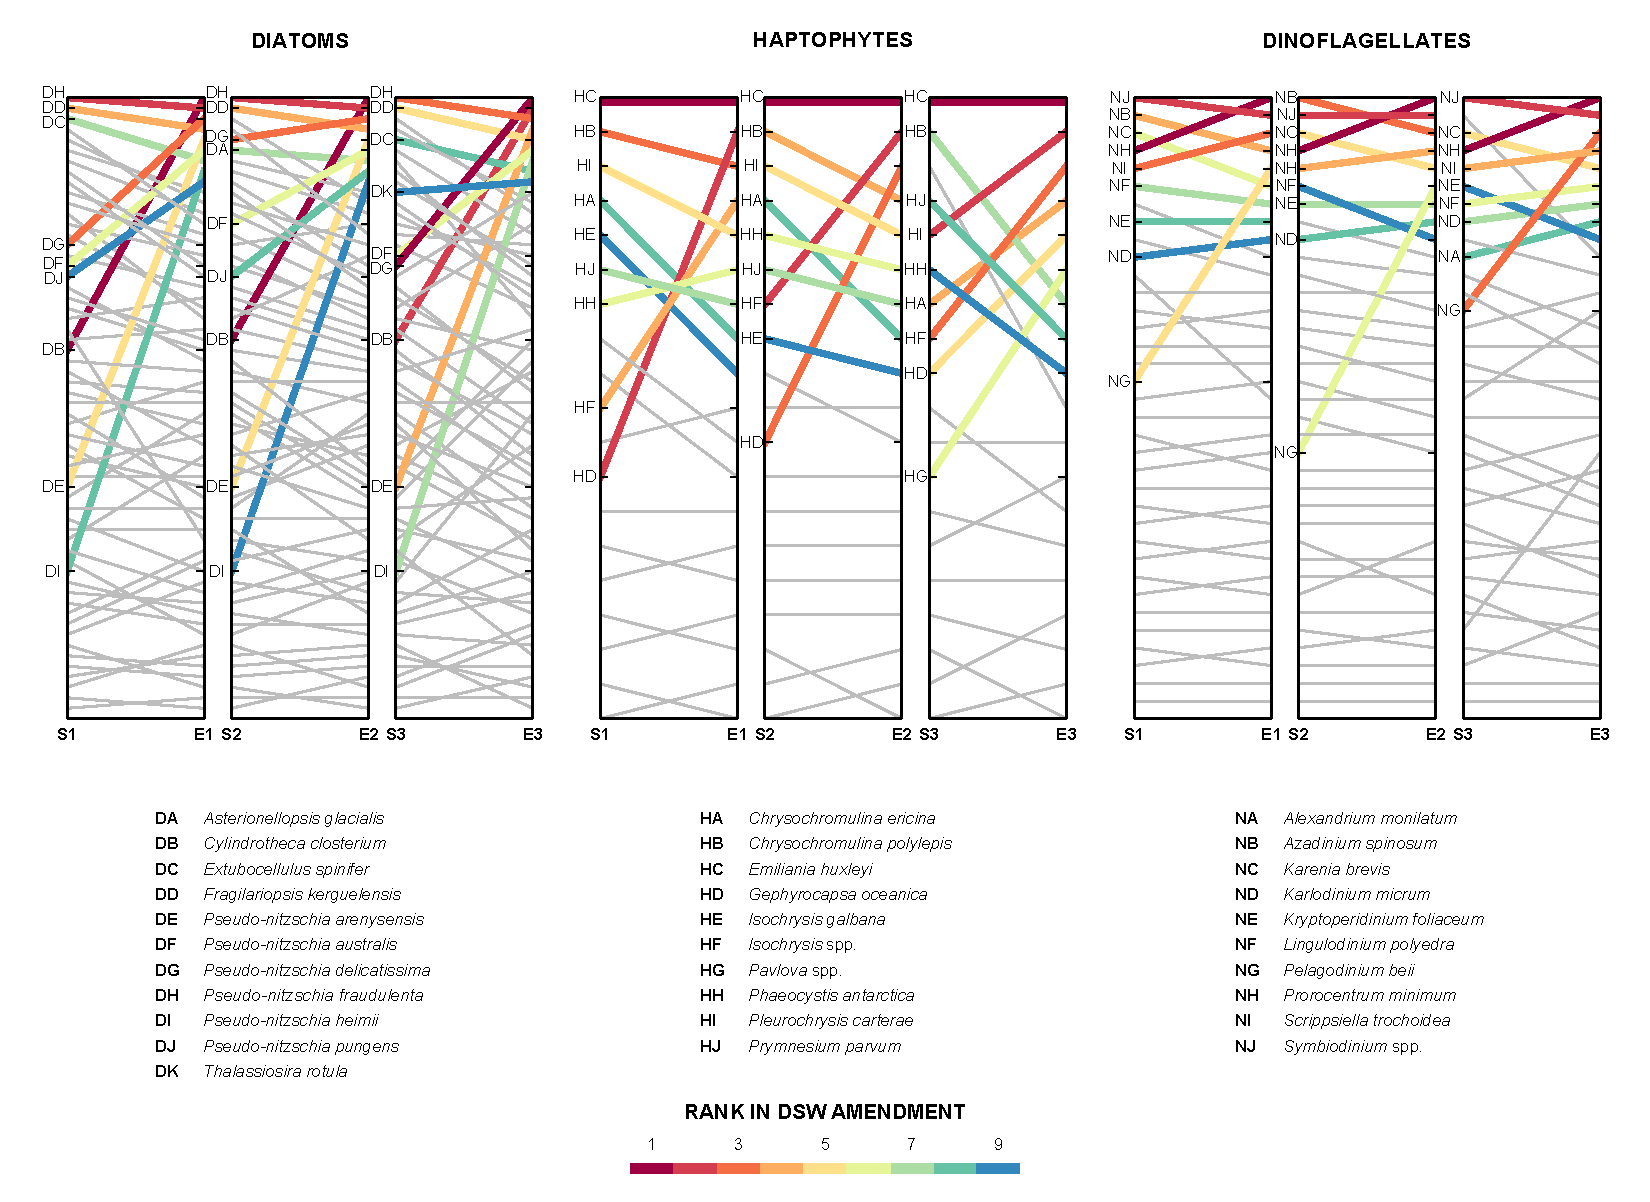
\includegraphics[width=1\textwidth]{Images/C4_FigureS2.pdf}
    \caption[Rank abundance shifts in the species composition of diatoms, haptophytes and dinoflagellates]{Rank abundance shifts in the species composition of diatoms, haptophytes and dinoflagellates for the three experiments. The relative shift in rank abundance for each species is depicted for each incubation experiment (E1-E3) following deep seawater (DSW) addition. The nine most abundant taxa following DSW addition are highlighted for each of the functional groups. Although the species that recruited the reads are denoted here this is highly driven by the composition of the database and does not necessarily indicate the actual species present, but rather the closest species present in the database.}
  \label{fig:a4f2}
\end{figure}

%Supplemental Figure 3: QMF Comparison across species


\begin{figure}[p!]
  \centering
    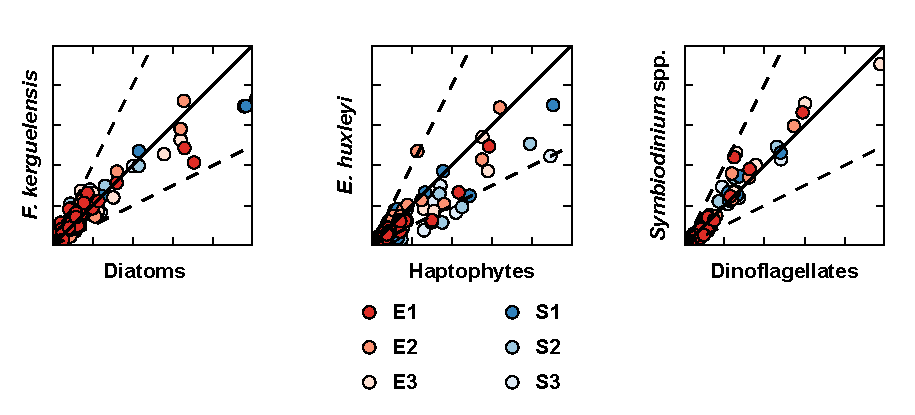
\includegraphics[width=1\textwidth]{Images/C4_FigureS3.pdf}
    \caption[Comparison of the quantitative metabolic fingerprint (QMF) between the whole functional group and representative taxa]{Comparison of the quantitative metabolic fingerprint (QMF) between the whole functional group and representative taxa. The proportion of reads falling into each of the modules depicted in Figure 2 is plotted for S1-S3 and E1-E3, comparing the summed functional group signal and that of a representative taxon. Color of the marker indicates the sample; solid and dashed lines mark the 1:1 and 1:2 lines, respectively.}
  \label{fig:a4f3}
\end{figure}

%Supplemental Figure 4: Distribution histogram

\begin{figure}[p!]
  \centering
    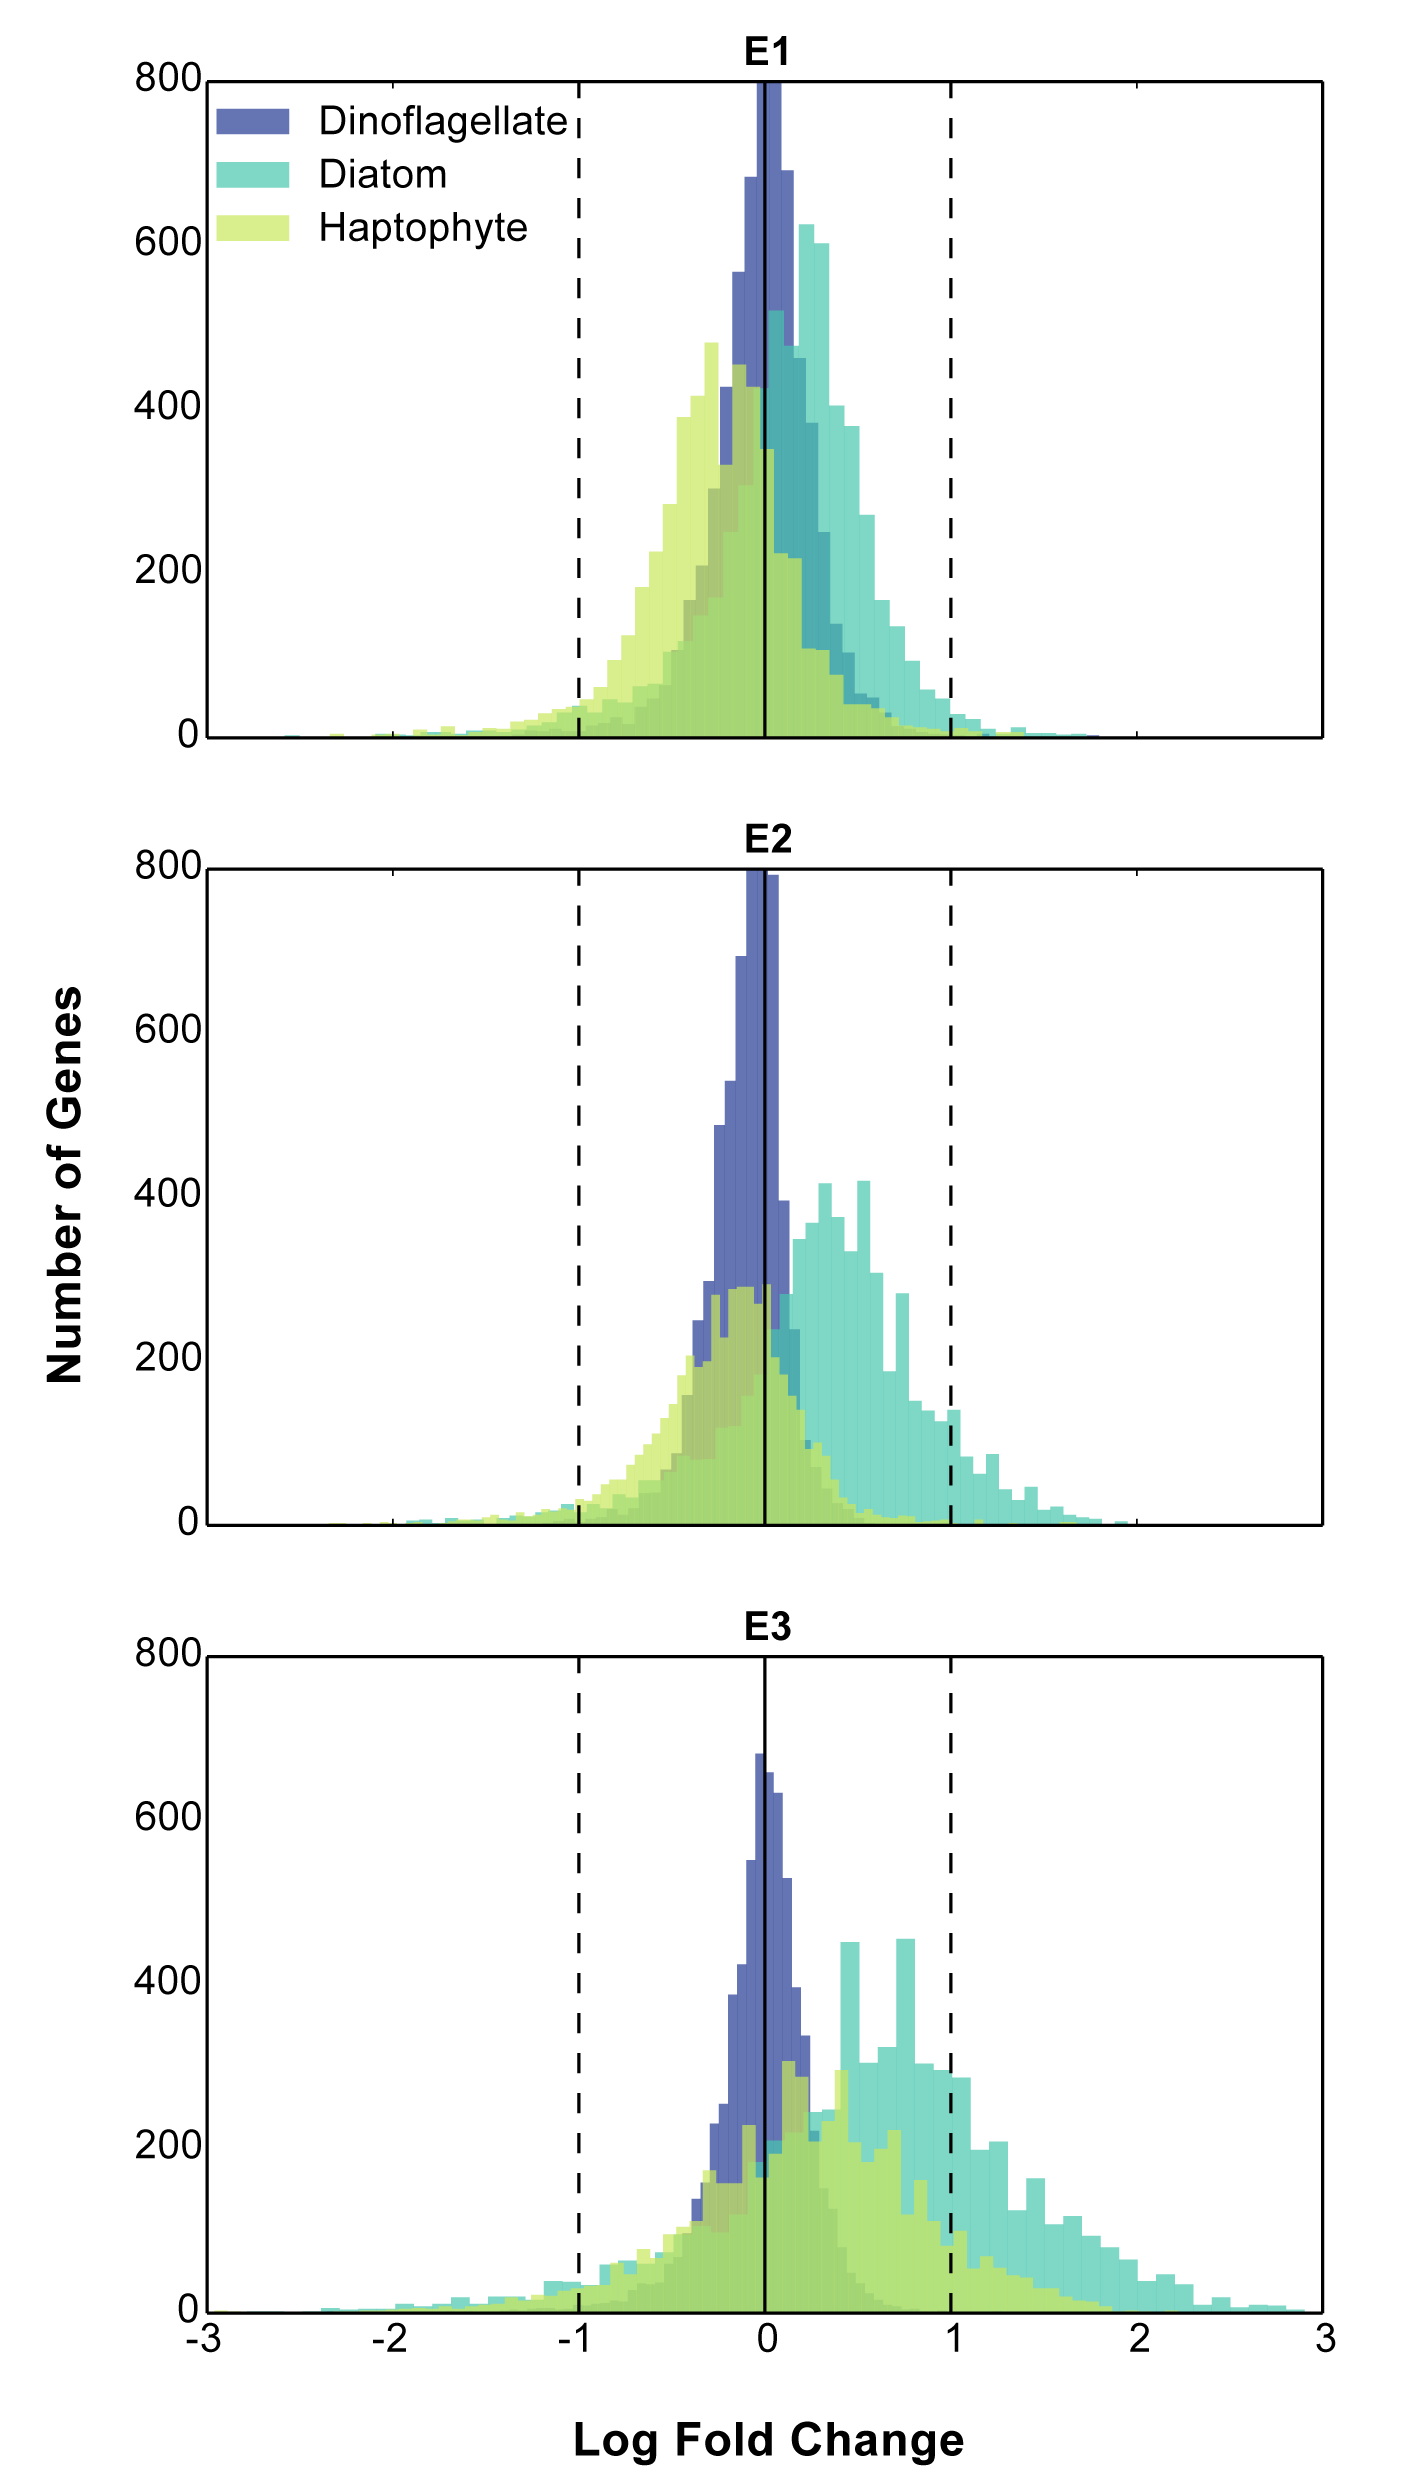
\includegraphics[width=.75\textwidth]{Images/C4_FigureS4.png}
    \caption[Distribution of log fold change following deep seawater (DSW) addition]{Distribution of log fold change following deep seawater (DSW) addition. Histogram of the number of genes falling within each of the log fold change bins for diatoms, haptophytes and dinoflagellates. Solid line indicates no fold change; dashed lines indicate 2 fold-change both up and down.}
  \label{fig:a4f4}
\end{figure}


%Supplemental Figure 5: Weight venn diagrams for up and down regulated genes

\begin{figure}[p!]
  \centering
    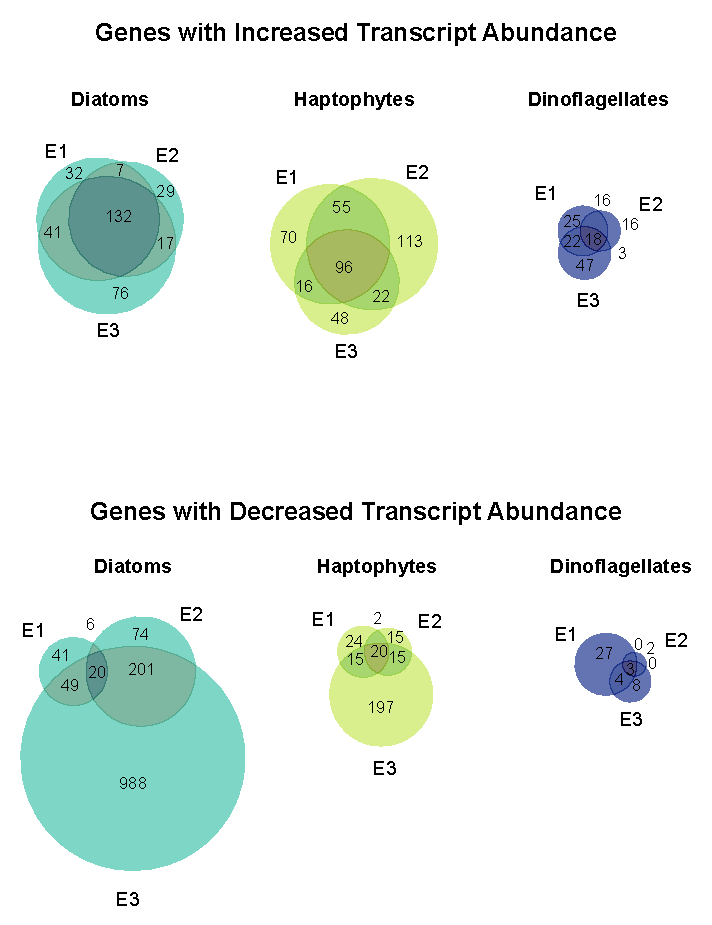
\includegraphics[width=1\textwidth]{Images/C4_FigureS5.pdf}
    \caption[Weighted Venn diagrams of genes with significantly different abundances following deep seawater (DSW) addition by functional group]{Weighted Venn diagrams of genes with significantly different abundances following deep seawater (DSW) addition by functional group. The uniqueness of KEGG orthologs with increased or decreased abundances as determined by ASC (2 fold-change, post-p > 0.95) across experiments was assessed for diatoms, haptophytes, and dinoflagellates.}
  \label{fig:a4f5}
\end{figure}


%Supplemental Figure 6: MANTA Plots

\begin{figure}[p!]
  \centering
    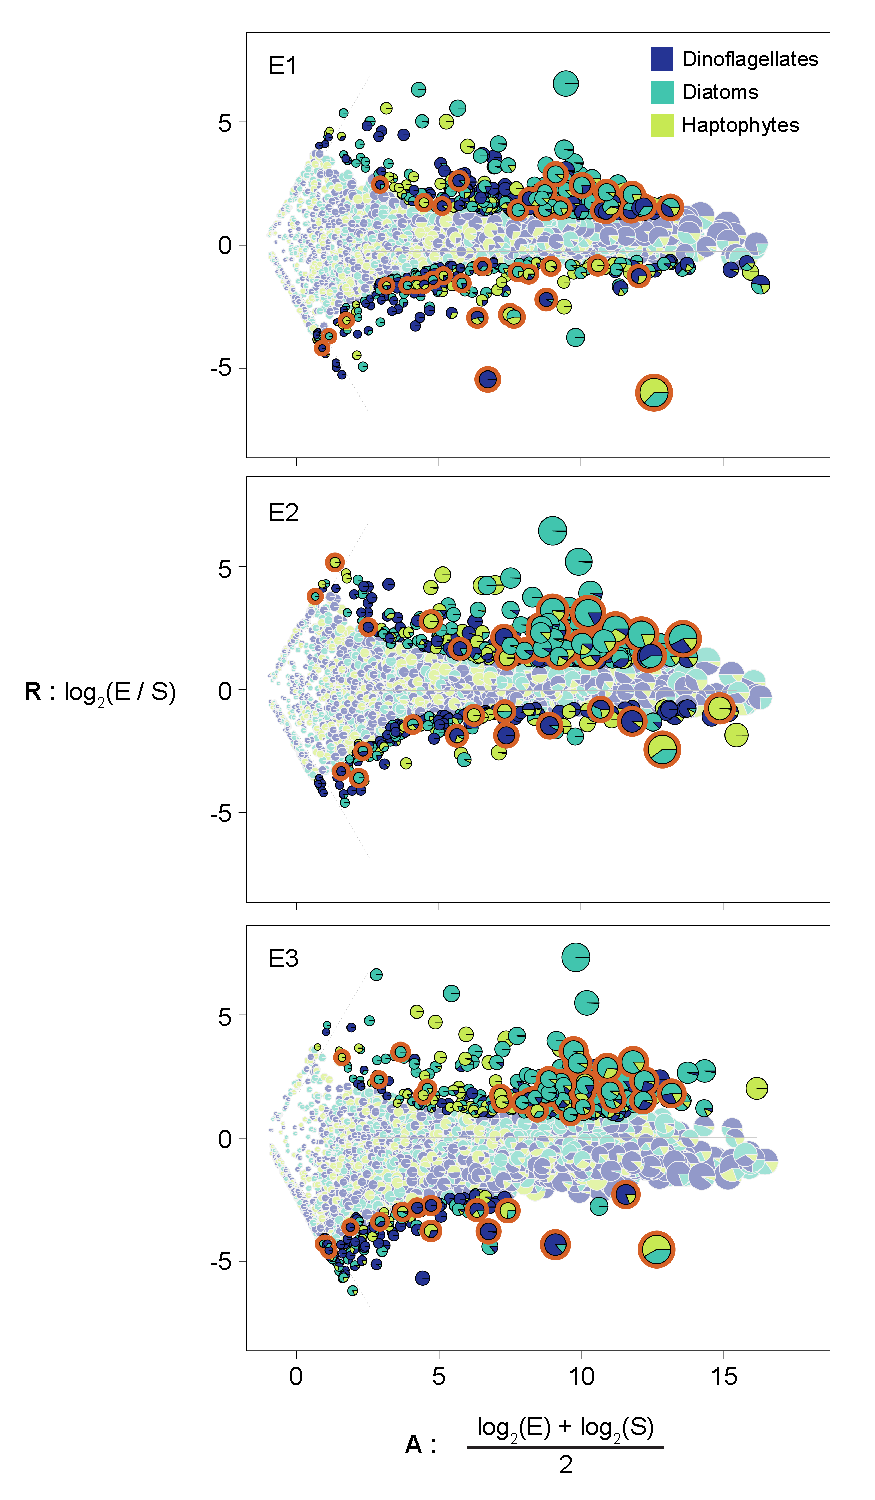
\includegraphics[width=.7\textwidth]{Images/C4_FigureS6.pdf}
    \caption[Microbial Assemblage Normalized Transcript Analysis (MANTA) ratio-averaged plots for global shifts in expression of KEGG orthologs]{Microbial Assemblage Normalized Transcript Analysis (MANTA) ratio-averaged plots for global shifts in expression of KEGG orthologs. Fold change ratio (R) and average read count (A) are plotted for read counts in the \emph{in situ} (S) and deep seawater (DSW) amendment (E) samples across the three sample pairs (S1:E1, S2:E2, S3:E3). The trimmed mean of fold-change values is noted as a gray solid line; orthologs unique to one library are separated by gray dashed lines. Pies indicate the taxonomic distribution of orthologous reads across the three functional groups. KEGG orthologs that were significantly differentially expressed (DE) (adjusted $P > 0.05$) are outlined in black and those not significantly DE are outlined in gray. DE KEGG orthologs that fall in the Energy Metabolism KEGG module are outlined in orange.}
  \label{fig:a4f6}
\end{figure}

%Supplemental Figure 7: QMF across incubation experiments

\begin{figure}[p!]
  \centering
    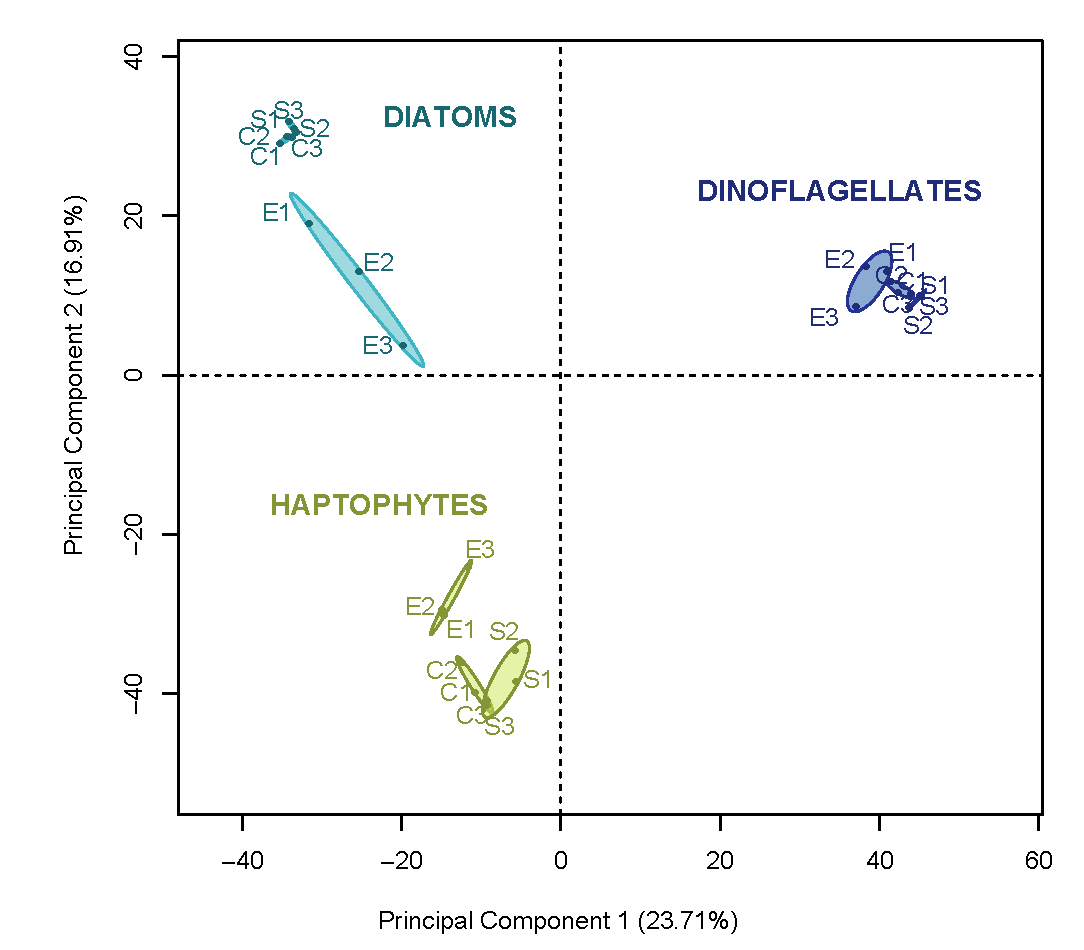
\includegraphics[width=1\textwidth]{Images/C4_FigureS7.pdf}
    \caption[Principal component analysis of the quantitative metabolic fingerprint (QMF) signals across \emph{in situ}, no addition control, and deep seawater amended samples]{Principal component analysis of the quantitative metabolic fingerprint (QMF) signals across \emph{in situ}, no addition control, and deep seawater (DSW) amended samples. Principal component analysis of the QMF signals for each of the functional groups across \emph{in situ} (S1-S3), control no addition (C1-C3) and DSW amendment (E1-E3); 95\% confidence ellipses are indicated for each of the sample types by functional group.}
  \label{fig:a4f7}
\end{figure}

\clearpage

\subsection{Supplemental Tables}

% Supplemental table with nutrient concentrations post treatment run for E and C
\begin{table}[h!]
\centering
\caption[Macronutrient concentrations in deep seawater ammendment and the incubation experiments after 168 hours]{Macronutrient concentrations in control no addition (C), DSW-amended incubations (E), and 700 m water used in DSW amendment incubations}
\label{tab:a4t1}
\newcolumntype{C}[1]{>{\centering\let\newline\\\arraybackslash\hspace{.5pt}}m{#1}}
\begin{tabular}{ccccc}

    
\hline
\multicolumn{1}{|c|}{\multirow{2}{*}{\textbf{Treatment}}} & \multicolumn{1}{c|}{\multirow{2}{*}{\textbf{\begin{tabular}[c]{@{}c@{}}Time post \\ inoculation (hours)\end{tabular}}}} & \multicolumn{1}{c|}{\multirow{2}{*}{\textbf{\begin{tabular}[c]{@{}c@{}}NO2 + NO3 \\ ($\mu M$)\end{tabular}}}} & \multicolumn{1}{c|}{\multirow{2}{*}{\textbf{\begin{tabular}[c]{@{}c@{}}PO4 \\ ($\mu M$)\end{tabular}}}} & \multicolumn{1}{c|}{\multirow{2}{*}{\textbf{\begin{tabular}[c]{@{}c@{}}Si\\ ($\mu M$)\end{tabular}}}} \\

\multicolumn{1}{|c|}{}                                    & \multicolumn{1}{c|}{}                                                        & \multicolumn{1}{c|}{}                                                                                    & \multicolumn{1}{c|}{}                                                                              & \multicolumn{1}{c|}{}                                                                            \\ \hline
\multicolumn{1}{|c|}{\textbf{C} (control no addition) *}  & \multicolumn{1}{c|}{168}                                                     & \multicolumn{1}{c|}{$0.12 \pm 0.03$}                                                                         & \multicolumn{1}{c|}{$0.12 \pm 0.02$}                                                                   & \multicolumn{1}{c|}{$1.91 \pm 0.2$}                                                                  \\ \hline
\multicolumn{1}{|c|}{\textbf{E} (+ 10\% DSW) *}           & \multicolumn{1}{c|}{168}                                                     & \multicolumn{1}{c|}{$1.9 \pm  .93$}                                                                          & \multicolumn{1}{c|}{$0.23 \pm 0.05$}                                                                   & \multicolumn{1}{c|}{$8.46 \pm 3.11$}                                                                 \\ \hline
\multicolumn{1}{|c|}{\textbf{DSW} (700 m water) *}        & \multicolumn{1}{c|}{N/A}                                                     & \multicolumn{1}{c|}{$37.5 \pm 1.68$}                                                                         & \multicolumn{1}{c|}{$3.14 \pm 0.03$}                                                                   & \multicolumn{1}{c|}{$83.4 \pm 9.33$}                                                                 \\ \hline
\multicolumn{5}{l}{\textit{* Nutrient data averaged for E1 and E2, nutrients were not assayed on E3.}}                                                                                                                                                                                                                                                                                                                                                     
\end{tabular}
\end{table}


%%%%%%%%%%%%%%%%%%%%%%%%%%%

%%%%%%%%%%%%%%%%%%%%%%%%%%%_________________CHAPTERTHREE_________________%%%%%%%%%%%%%%%%%%%%%%%%%%%

%%%%%%%%%%%%%%%%%%%%%%%%%%%

\chapter{Chapter 3 Supplemental Information}
\label{sec:app3}
\clearpage
\section{Supplemental Figures}

%Supplemental Figure 1: Cell counts in NB 
\begin{figure}[h!]
  \centering
    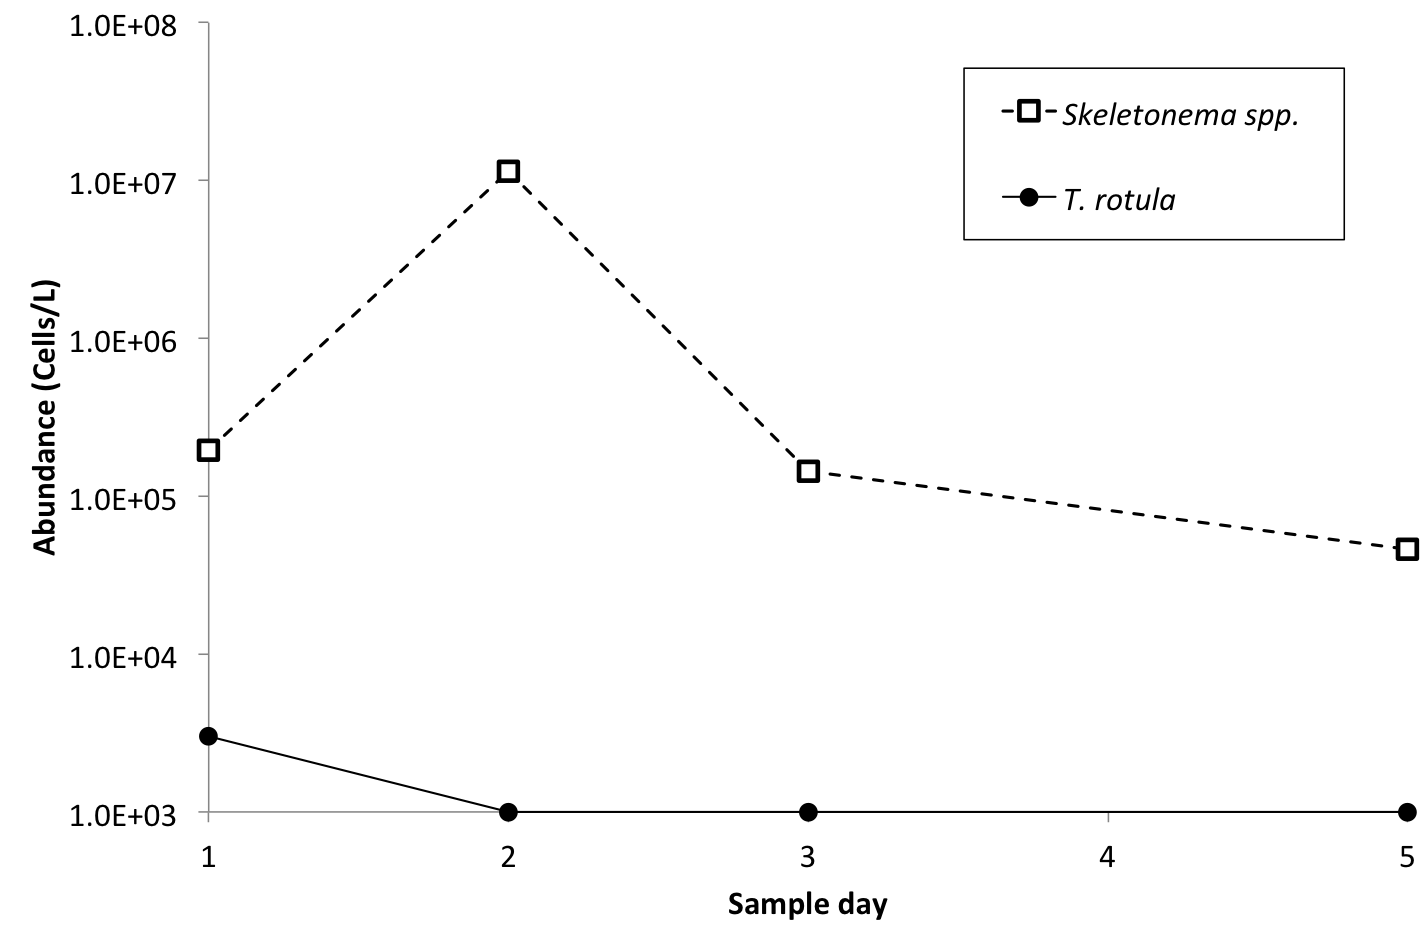
\includegraphics[width=1\textwidth]{Images/C3_SFigure1_CellCounts.png}
    \caption[Cell counts in Narragansett Bay during the spring of 2012]{Abundance estimation from cell counts of \textit{Skeletonema} spp. and \textit{T. rotula} across the five sample points during the spring of 2012. }
  \label{fig:a3f1}
\end{figure}


%Supplemental Figure 2: KEGG linear correlation
\begin{figure}[p!]
  \centering
    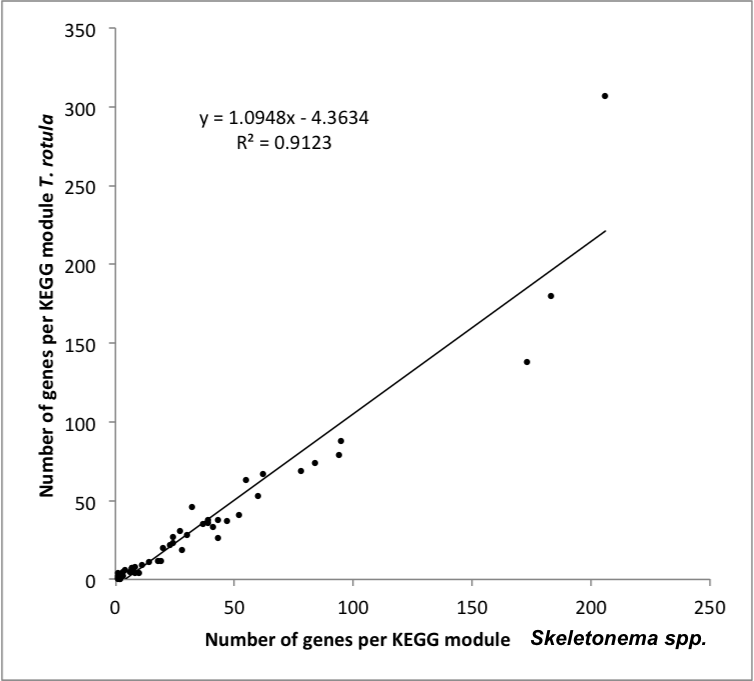
\includegraphics[width=1\textwidth]{Images/C3_SFigure2_KEGGModuleGeneContent2.png}
    \caption[Comparison of KEGG module content between \textit{Skeletonema} spp. and \textit{T. rotula} ]{Total number of genes assigned to each KEGG module for \textit{Skeletonema} spp. and \textit{T. rotula}.}
  \label{fig:a3f2}
\end{figure}


%Supplemental Figure 3: Hierarchical clustering of S and T across time
\begin{figure}[p!]
  \centering
    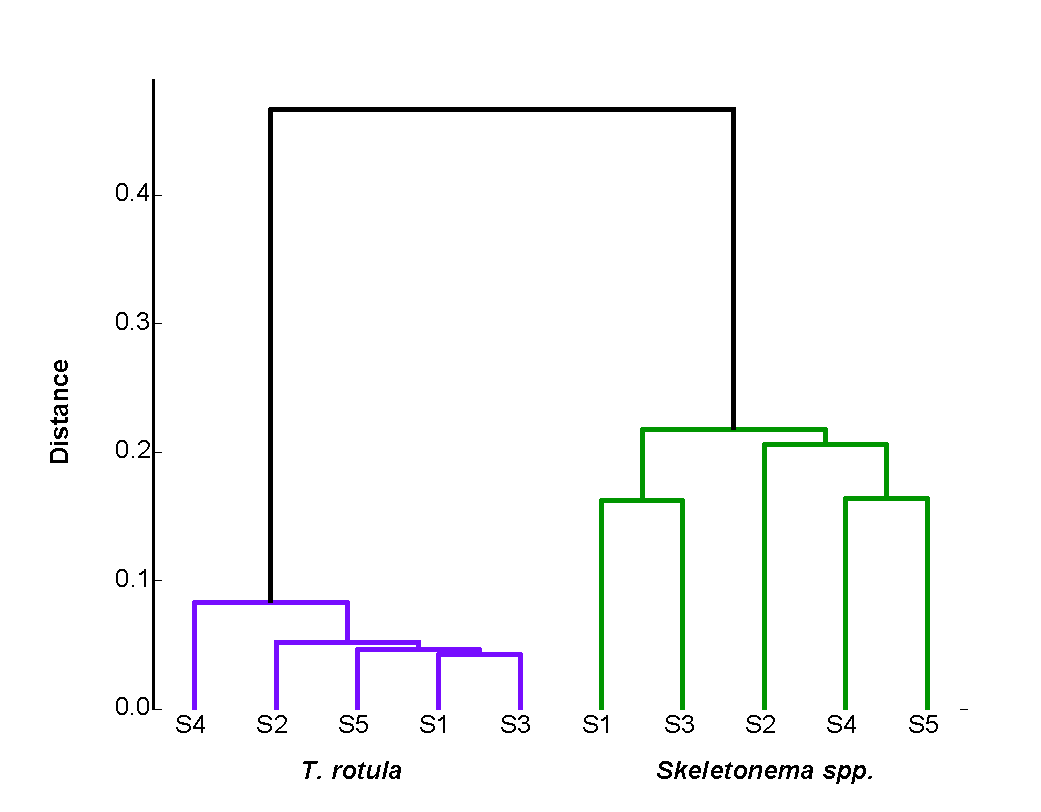
\includegraphics[width=1\textwidth]{Images/C3_SFigure3_Dendrogram.pdf}
    \caption[Hierarchical clustering of QMF signatures across species and samples]{Dendrogram depicting hierarchical clustering of samples based on relative expression of KEGG modules (Figure 2) across the five samples S1-S5 for \textit{Skeletonema} spp. and \textit{T. rotula}.}
  \label{fig:a3f3}
\end{figure}

%Supplemental Figure 4: Stable gene expression across time
\begin{figure}[p!]
  \centering
    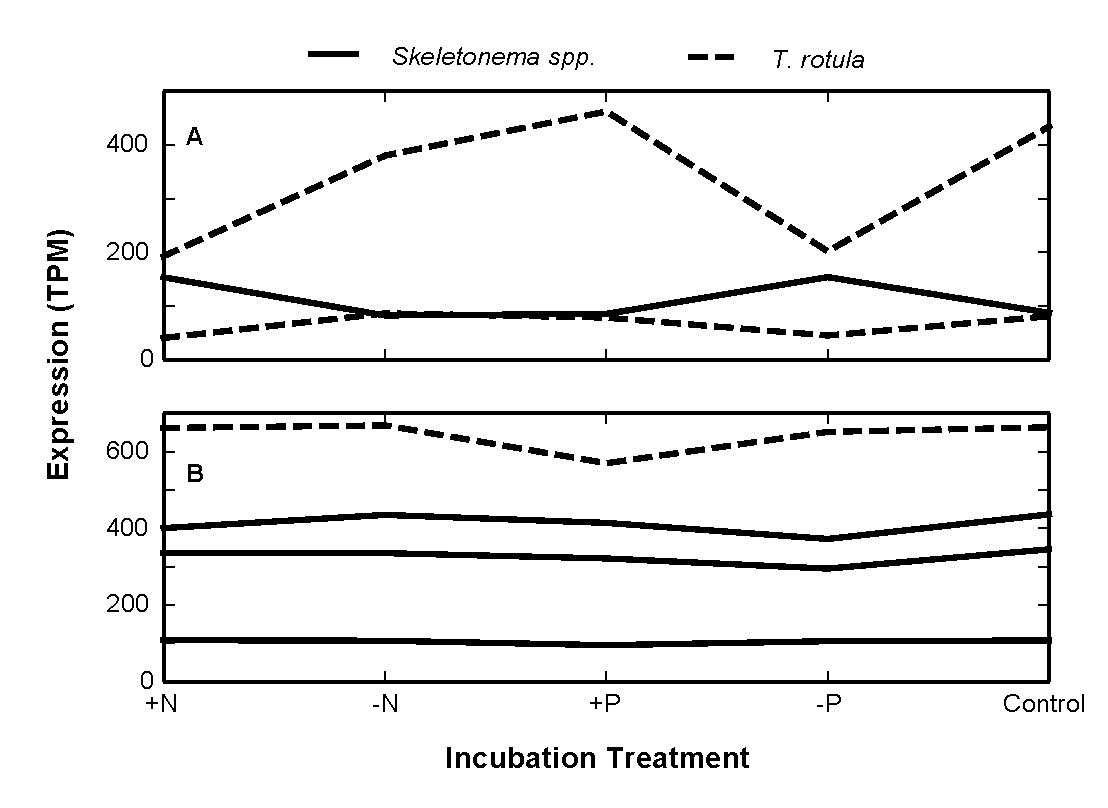
\includegraphics[width=1\textwidth]{Images/C3_SFigure4_StableGenePlot_wActin.pdf}
    \caption[Expression of stable reference genes in the field]{Expression of stable reference genes identified based on literature and statistical parsing in nutrient amendment incubation. (A) The expression in tags per million ($TPM$) of stable reference genes identified in \textit{T. rotula} (dashed line) and \textit{Skeletonema} spp.  (solid lines) based on homology (e-value < 1e-5) to a known reference genes in \textit{T. pseudonana}, ACT1 (Thaps\_25772), in nutrient incubations. (B) Also shown are reference genes identified in the incubation experiments, using statistical analysis of sequence counts \citep{Alexander2012, Wu2010}, and nutrient incubations }
  \label{fig:a3f4}
\end{figure}

%Supplemental Figure 5: RR gene composition
\begin{figure}[p!]
  \centering
    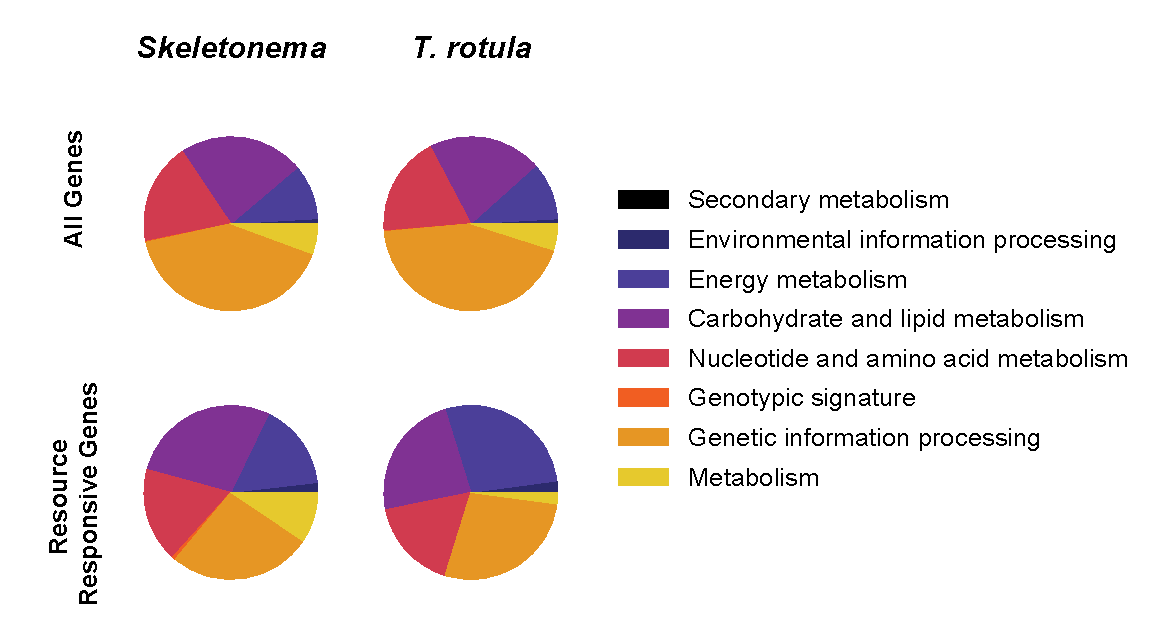
\includegraphics[width=1\textwidth]{Images/C3_SFigure5_RR_All_Genes_Pie.pdf}
    \caption[Functional compoosition of the reference transcriptome and resource-responsive gene sets]{Functional composition of the reference transcriptome and resource-responsive (RR) gene subset for \textit{T. rotula} and \textit{Skeletonema} spp. (A) RR gene sets were identified through cross comparison of like-nutrient incubations (i.e. +N vs. -N and +P vs. -P), using ASC (fold change = 2, post-$p > 0.95$). The relative functional categorization of the reference transcriptomes and RR gene set for \textit{T. rotula} and \textit{Skeletonema} spp. based on KEGG ontology as assigned by KAAS is depicted at the module-level.}
  \label{fig:a3f5}
\end{figure}

%Supplemental Figure 6: Expression of nitrate reductase

\begin{figure}[p!]
  \centering
    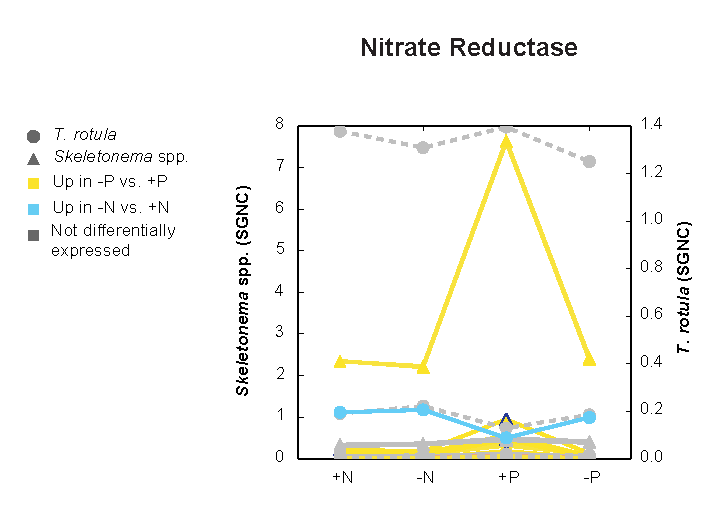
\includegraphics[width=1\textwidth]{Images/C3_SFigure6_SGNC_NitrateReductase.pdf}
    \caption[Relative expression of nitrate reducatses across incubation experiments]{The relative expression in stable gene normalized counts ($SGNC$) of the assimilatory nitrate reductase gene cluster across the incubation experiment treatments. Significance of regulation between the treatments is denoted by the color of the line; organisms are denoted by the shapes of the marker.}
  \label{fig:a3f6}
\end{figure}

%Supplemental Figure 7: Cluster Analysis


\begin{figure}[p!]
  \centering
    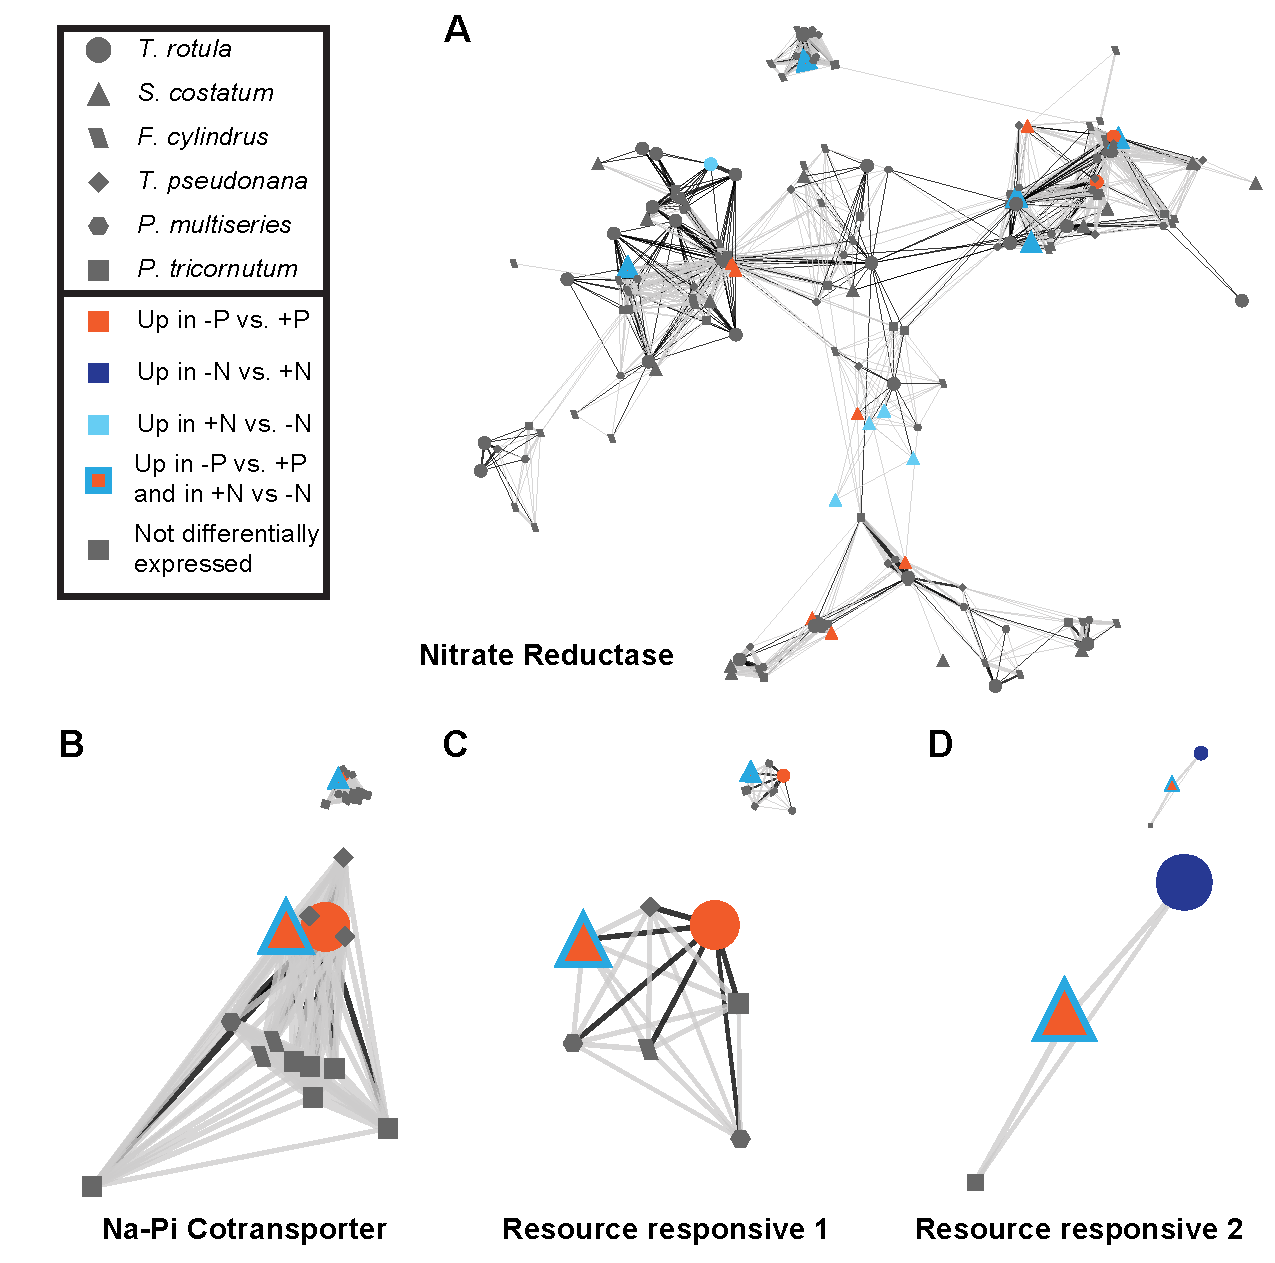
\includegraphics[width=1\textwidth]{Images/C3_SFigure7_ClusterAnalysis_v5.pdf}
    \caption[Gene cluster analysis of nutrient-responsive genes]{Gene cluster known nutrient-responsive genes in \textit{T. pseudonana}: (A) assimilatory nitrate reductase and (B) sodium-phosphate cotransporter and novel resource-responsive (RR) gene families: (C) RR1 and (D) RR2. Transcripts from the transcriptomes of \textit{T. rotula} and \textit{Skeletonema} spp. were clustered based upon relative homology with available diatom genomes: \textit{F. cylindrus}, \textit{P. tricornitum}, \textit{P. multiseries}, and \textit{T. pseudonana}. Symbols indicate different species, while color indicates regulation in the field incubation experiments. Two nodes within a gene cluster are connected by an edge if they share a homologous protein (reciprocal BLAST hit with a minimum of 1e-5 score and minimum 20\% identity). Gene clusters are visualized using an edge-weighted spring-embedded model based on e-value, meaning that genes that are closer together are more similar. The width of the line correlates to the magnitude of the e-value, with lower e-values represented by thicker lines and higher e-values represented by thinner lines.}
  \label{fig:a3f7}
\end{figure}

%Supplemental Figure 8: Conceptual schematic of STD niche space

\begin{figure}[p!]
  \centering
    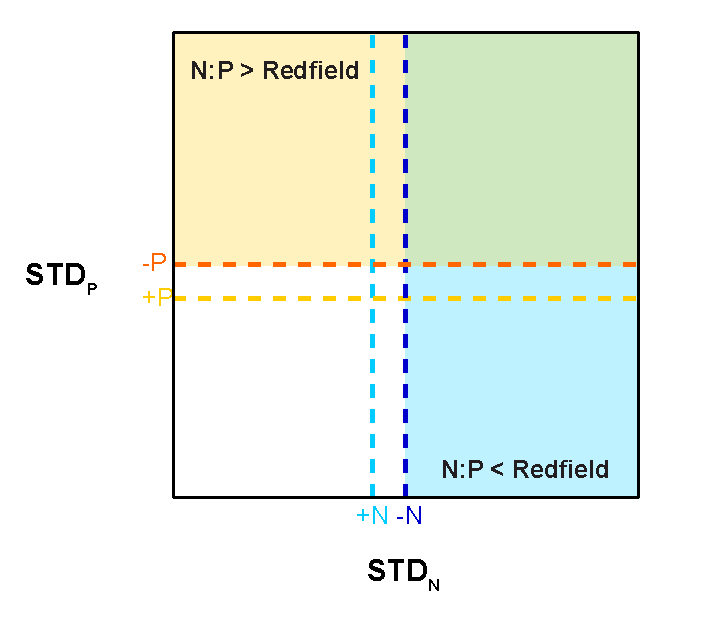
\includegraphics[width=1\textwidth]{Images/C3_SFigure8_Schematic_Quadrants.pdf}
    \caption[Conceptual schemiatic of $STD_N$ plotted against $STD_P$]{A conceptual schematic of $STD_N$ plotted against $STD_P$ hypothesized regions of N:P > Redfield physiology and N:P < Redfield physiology highlighted.}
  \label{fig:a3f8}
\end{figure}


%Supplemental Figure 9: NISP Dn genes
\begin{landscape}
   \centering
   \null         %%<---- this is needed
   \vfill        %%<-----here

	\begin{figure}
  	\centering
    	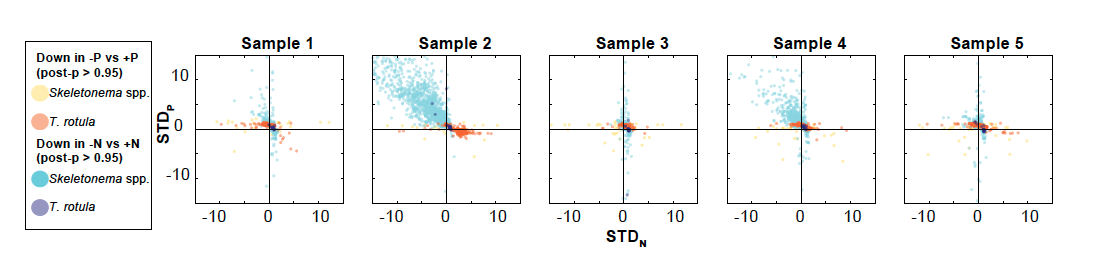
\includegraphics[width=1.3\textwidth]{Images/C3_SFigure9_NISP_DNGenes.png}
    	\caption[Evolution of niche space indexing over for significantly down-regualted genes]{Evolution of niche space indexing over time in Narragansett Bay for \textit{T. rotula} and \textit{Skeletonema} spp.. The stable gene normalized field signal from genes identified as significantly (2-fold change, post$-p > 0.95$) down-regulated in -P vs +P for Skeletonema spp. (yellow) and \textit{T. rotula} (orange) and in -N vs +N for for \textit{Skeletonema} spp. (cyan) and \textit{T. rotula} (dark blue) was proportionalized relative to the expression for those genes in nutrient incubations, yielding the $STD_N$ and $STD_P$. These data are plotted for Sample 1 through Sample 5.}
  	\label{fig:a3f9}
	\end{figure}
    \vfill        %%<----- and here
\end{landscape}

%Supplemental Figure 10: Percentage of RR genes by quadrant

\begin{figure}[h!]
  \centering
    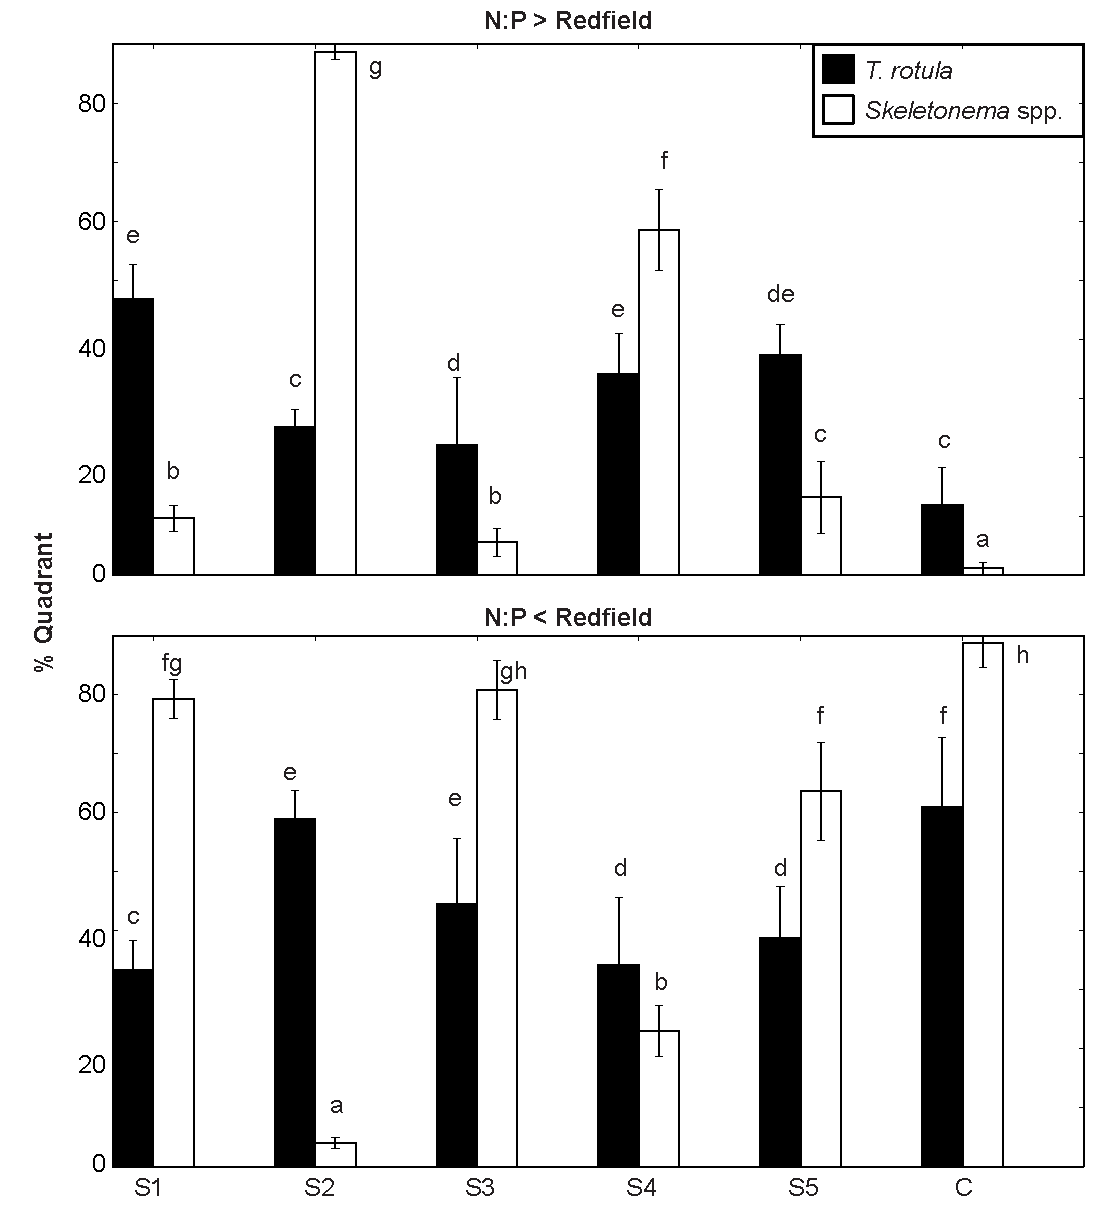
\includegraphics[width=1\textwidth]{Images/C3_SFigure10_BarGraph_Quadrant_2575_stats.pdf}
    \caption[The percentage of identified nutrient responsive genes falling into the N:P > Redfield and N:P < Redfield quadrants with varried cutoffs]{The percentage of identified nutrient responsive genes falling into the N:P > Redfield and N:P < Redfield quadrants for \textit{T. rotula} and \textit{Skeletonema} spp.. The total number of genes falling into the N:P > Redfield quadrant ($STD_P > C$; $STD_N < C$, for $0.25 < C < 0.75$) and the N:P < Redfield quadrant ($STD_P$ < C; $STD_N > C$, for $0.25 < C < 0.75$). The value of C was varied over 10 different values and the average percentages of genes falling into each of the quadrants is depicted above based on the size of the circle at the median $STD_N$ and $STD_P$ for the genes in the quadrant. Similarity of data between species by quadrant was assessed using an analysis of variance (ANOVA) with a generalized linear model. The results from a post hoc Tukey test show the divergence of species across time ($p < 0.05$).}
  \label{fig:a3f10}
\end{figure}

%Supplemental Figure 11: Quadrant localization with varying stable reference genes

\begin{figure}[p!]
  \centering
    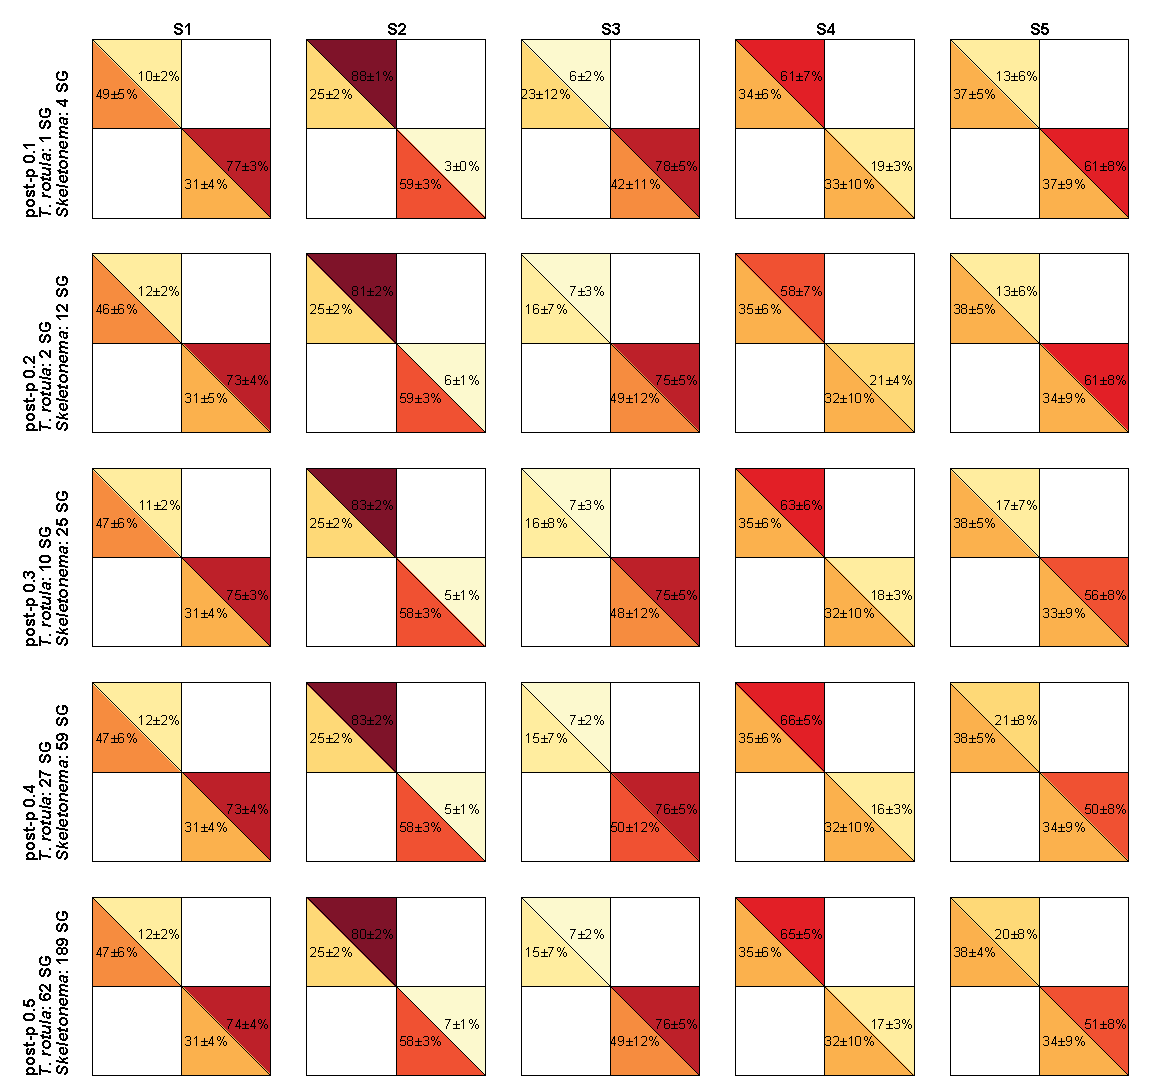
\includegraphics[width=1\textwidth]{Images/C3_SFigure11_Quadrant.pdf}
    \caption[The impact of stable gene selction of quadrant localization]{The impact of stable gene selection on the quadrant localization of the resource responsive gene sets. The posterior probability cutoff used in the selection of stable genes was varied from 0.1 to 0.5 for a fold change of 1.25. The percentage of identified nutrient responsive genes falling into the N:P > Redfield and N:P < Redfield quadrants for \textit{T. rotula} and \textit{Skeletonema} spp. across the five sample points and five posterior probability values is depicted.}
  \label{fig:a3f11}
\end{figure}



\section{Supplemental Tables}

%Supplemental Table 1: library stats

\begin{table}[h!]
\centering
\caption[The total number of paired end reads after quality control and trimming and the percentage of reads mapping]{The total number of paired end reads after quality control and trimming and the percentage of reads mapping to the \textit{T. pseudonana} genome, \textit{T. rotula} transcriptome, and \textit{S. costatum} transcriptome.}
\label{tab:a3t1}
\newcolumntype{L}[1]{>{\raggedright\let\newline\\\arraybackslash\hspace{0pt}}m{#1}}
\label{my-label}
\begin{tabular}{lp{2cm}lll}
\multirow{2}{*}{Sample} & \multirow{2}{*}{\parbox{2cm}{Library Size (PE reads)}} & \multicolumn{3}{c}{\textbf{Representation in library}}             \\ 
                        &                                          & \textit{T. pseudonana} & \textit{T. rotula} & \textit{S. costatum} \\ \Xhline{2\arrayrulewidth}
S1                      & 89455034                                 & 2.98\%                 & 17.50\%            & 33.50\%              \\ \hline
S2                      & 64888267                                 & 0.41\%                 & 11.70\%            & 54.90\%              \\ \hline
S3                      & 103250243                                & 0.39\%                 & 7.30\%             & 9.00\%               \\ \hline
S4                      & 45370867                                 & 0.68\%                 & 8.80\%             & 8.30\%               \\ \hline
S5                      & 55061692                                 & 0.88\%                 & 10.40\%            & 11.20\%              \\ \hline
Ambient Control         & 51508197                                 & 0.27\%                 & 13.40\%            & 8.00\%               \\ \hline
+N                      & 58626239                                 & 0.43\%                 & 6.10\%             & 5.30\%               \\ \hline
-N                      & 44561851                                 & 0.41\%                 & 8.70\%             & 8.30\%               \\ \hline
+P                      & 51130364                                 & 0.29\%                 & 8.50\%             & 8.00\%               \\ \hline
-P                      & 58834022                                 & 0.40\%                 & 6.60\%             & 6.50\%               \\ \hline
\end{tabular}
\end{table}

%Supplememntal Table 2: nutrient concentrations used in incubations

\begin{table}[h!]
\centering
\caption[Nutrient concentrations used in nutrient amendment incubations. ]{Nutrient concentrations used in nutrient amendment incubations.}
\label{tab:a3t2}
\begin{tabular}{llllll}
            & \multicolumn{5}{c}{Treatment}                                        \\
Amendment   & Ambient Control & +N         & +P        & -N          & -P          \\\Xhline{2\arrayrulewidth}
Nitrate     & -               & $10 \mu M$ & -         & -           & $10 \mu M$  \\
Phosphate   & -               & -          & $3 \mu M$ & $3 \mu M$   & -           \\
Silica      & -               & -          & -         & $68 \mu M$  & $68 \mu M$  \\
Iron        & -               & -          & -         & $4.6 \mu M$ & $4.6 \mu M$ \\
Vitamin B12 & -               & -          & -         & f/5         & f/5        
\end{tabular}
\end{table}

%Supplememntal Table 3: nutrient concentrations used in incubations

\begin{table}[h!]
\centering
\caption[Mapping statistics for \textit{T. rotula} and \textit{S. costatum} transcriptomes]{Total number of contigs in the \textit{T. rotula} and \textit{S. costatum} transcriptomes and the number of genes in each of the differentially regulated and stable groupings.}
\label{tab:a3t3}
\newcolumntype{L}[1]{>{\raggedright\let\newline\\\arraybackslash\hspace{0pt}}m{#1}}
\begin{tabular}{L{3.5cm}ll}
\hline
                                                                       & \textit{\textbf{T. rotula}} & \textit{\textbf{S. costatum}} \\ \Xhline{2\arrayrulewidth}

Number of contigs in transcriptome                                     & 22362                       & 27665                         \\ \hline
Pass 2 TPM cutoff                                                      & 4318                        & 20921                         \\ \hline
Up in -P vs +P                                                         & 249                         & 4754                          \\ \hline
Down in -P vs +P                                                       & 335                         & 52                            \\ \hline
Up in -N vs +N                                                         & 196                         & 9                             \\ \hline
Down in -N vs +N                                                       & 49                          & 1631                          \\ \hline
All differentially regulated (2 fold change, post-$p > 0.95$) & 775                         & 5136                          \\ \hline
Stable genes (1.25 fold change, post-$p < 0.1$)                  & 1                           & 4                             \\ \hline
\end{tabular}
\end{table}

\clearpage

\section{Supplemental Data}

    \begin{DS3}
    
    \item \label{DS31}: Annotations based on KEGG Ontology for \textit{Skeletonema} spp. and \textit{T. rotula} transcriptomes. \href{http://www.pnas.org/content/suppl/2015/04/09/1421993112.DCSupplemental/pnas.1421993112.sd01.xlsx}{Data Sheet 3-1} can be downloaded from the online version of the manuscript of \citet{Alexander2015} through \href{http://www.pnas.org/content/112/17/E2182.full}{\textit{Proceedings of the National Academy of Sciences}}. 
    \item \label{DS32}: Relative expression in tags per million (TPM) for genes identified as differentially or stably expressed in nutrient incubations. \href{http://www.pnas.org/content/suppl/2015/04/09/1421993112.DCSupplemental/pnas.1421993112.sd02.xlsx}{Data Sheet 3-2} can be downloaded from the online version of the manuscript of \citet{Alexander2015} through \href{http://www.pnas.org/content/112/17/E2182.full}{\textit{Proceedings of the National Academy of Sciences}}. 
  
    \end{DS3}



%% This defines the bibliography file (main.bib) and the bibliography style.
%% If you want to create a bibliography file by hand, change the contents of
%% this file to a `thebibliography' environment.  For more information 
%% see section 4.3 of the LaTeX manual.
\begin{singlespace}
\bibliography{main}
\bibliographystyle{myplainnat}
\end{singlespace}

\end{document}

